% arara: pdflatex
% arara: bibtex
% arara: bibtex
% arara: pdflatex

\documentclass{dcthesis}

%This version of the thesis template has been updated for the February 2017 thesis guidelines provided by the School of Graduate and Advanced Studies by David Freund and Daryl DeFord.

%  Some good options are draft and singlespacing, for drafts, and *final*,
%for the final cut, and noheadings, for a printout without headings.  
%You can also use the copyright option to add a copyright.  Note:
%final will enforce a bunch of different options, like oneside, 12pt
%and doublespacing, as well as make the margins correct.   Draft, has
%larger margins and is appropriate for two sided printing.   


%%%%%%%%%%%%%%%%%%%%%%%%%%%
%%%%    IMPORTANT     %%%%%
%%%%%%%%%%%%%%%%%%%%%%%%%%%
%
%  Because dvips doesn't know/care about the page size of the dvi file
%  its working on, and because its so important that the margins of
%  your thesis are correct you have to make sure that you are using
%  the command dvi -t letter *thesisnamehere*
%
%  If you are using a terminal this is straightforward, but if you are
%  using a tex editing program it make take a little bit of searching
%  before you figure out how to make this work. 
%  
%  Alternatively, you might consider compiling using pdflatex, which
%  compiles straight to a PDF and doesn't have this problem.  

%%%%%%%%%%%%%%%%%%%%%%%%%%%%%%%%%%%%%%%%%%%%%%%%%%
% Some Defaults
%%%%%%%%%%%%%%%%%%%%%%%%%%%%%%%%%%%%%%%%%%%%%%%%%%
\committee[F. Jon Kull, Ph.D.]{}{}{}{}
\school{Dartmouth College}{Hanover, New Hampshire}
\degree{Doctor of Philosophy}
\field{Mathematics}

%%%%%%%%%%%%%%%%%%%%%%%%%%%%%%%%%%%%%%%%%%%%%%%%%%
% Additional Packages (add as desired)
%%%%%%%%%%%%%%%%%%%%%%%%%%%%%%%%%%%%%%%%%%%%%%%%%%
\usepackage{amsmath,amssymb,amsthm,amsxtra}
% \usepackage{showkeys}
\usepackage{chngcntr}
\usepackage{mathrsfs} 
\usepackage{lipsum}
\usepackage{xcolor}
\usepackage{hyperref}
\hypersetup{colorlinks=true,urlcolor=blue,citecolor=blue,linkcolor=blue}
\usepackage{tikz}
\usepackage{colonequals}
\usepackage{enumerate}
\usepackage{booktabs}
\usepackage{longtable}
\usetikzlibrary{arrows,calc,automata,shadows,backgrounds,positioning,intersections,fadings,decorations.pathreplacing,shapes,matrix}
\usepackage{tikz-cd}
\tikzset{commutative diagrams/.cd, arrow style = tikz, diagrams = {>=latex}}
\tikzset{>=latex}
\usepackage{filecontents}
\usepackage{pgfplots, pgfplotstable}
\usepgfplotslibrary{statistics}

%%%%%% begin TCOLORBOX
\usepackage{tcolorbox, listings}
% \lstdefinestyle{mystyle}{
%   basicstyle=\ttfamily
% %  basicstyle=\ttfamily,
% %  numbers=left,
% %  numberstyle=\tiny,
% %  numbersep=5pt
% }
\tcbuselibrary{listings, skins, breakable}
\newtcblisting{code}{%
  title={\textsf{Magma}},
  %every listing line={\textcolor{blue}{\texttt{> }}},
  arc=0mm,
  top=0mm,
  bottom=0mm,
  left=3mm,
  right=0mm,
  width=\textwidth,
  boxrule=0.5pt,
  colback=gray!20,
  %spartan,
  listing only,
  % listing options={style=mystyle},
  breakable
}
%%%%%% end TCOLORBOX

%\usepackage{index} %Uncomment if you would like to have an index. Compiling with an index takes more work than compiling without one. You will have to look up how to use the index package.

%%%%%%%%%%%%%%%%%%%%%%%%%%%%%%%%%%%%%%%%%%%%%%%%%%
%Formatting
%%%%%%%%%%%%%%%%%%%%%%%%%%%%%%%%%%%%%%%%%%%%%%%%%%
%  Change or add to as desired. 
%  These two commands make the first enumerations look like (a)
%  And the second level like (i).  
% \renewcommand{\labelenumi}{(\alph{enumi})}
% \renewcommand{\labelenumii}{(\roman{enumii})}
%  These commands make the section headings Boldface and not all
%  caps. It also removes the chapter numbers  
\renewcommand{\chaptermark}[1]{\markboth{{\sc #1}}{{\sc #1}}}
\renewcommand{\sectionmark}[1]{\markright{{\sc \thesection\ #1}}}
%  These commands have lowercase headings with chapter numbers. 
%\renewcommand{\chaptermark}[1]{markboth{#1}{}}
%\renewcommand{\sectionmark}[1]{\markright{\thesection\ #1}} 
\newcommand{\PP}{\mathbb P}
\newcommand{\CC}{\mathbb C}
\newcommand{\RR}{\mathbb R}
\newcommand{\QQ}{\mathbb Q}
\newcommand{\ZZ}{\mathbb Z}
\renewcommand{\AA}{\mathbb A}
\newcommand{\defi}[1]{\textsf{#1}}
\newcommand{\jv}[1]{{\color{red} \sf JV: [#1]}}
\newcommand{\mm}[1]{{\color{blue} \sf MM: [#1]}}
\newcommand{\wt}[1]{\widetilde{#1}}
\newcommand{\QQal}{{\mathbb Q}^{\textup{al}}}
\newcommand{\FFqal}{{\mathbb F}_q^{\textup{al}}}
\newcommand{\QQab}{{\mathbb Q}^{\textup{ab}}}
\newcommand{\QQbar}{{\mathbb Q}^{\textup{al}}}
\newcommand{\Kal}{{{K}^{\textup{al}}}}
\newcommand{\Kab}{{K}^{\textup{ab}}}
\newcommand{\kbar}{\overline{k}}
\newcommand{\Kbar}{\overline{K}}
\newcommand{\LL}{\mathscr L}
\newcommand{\sm}{\setminus}
\newcommand{\FF}{\mathbb{F}}
\renewcommand{\ker}{\operatorname{ker}}

\DeclareMathOperator{\Div}{Div}
\DeclareMathOperator{\Pic}{Pic}
\DeclareMathOperator{\ddiv}{div}
\DeclareMathOperator{\sat}{sat}
\DeclareMathOperator{\ddeg}{deg}
\DeclareMathOperator{\ddim}{dim}
\DeclareMathOperator{\rred}{red}
% \renewcommand{\rred}{\operatorname{red}}
\DeclareMathOperator{\Lifts}{Lifts}
\DeclareMathOperator{\order}{order}
\DeclareMathOperator{\Aut}{Aut}
\DeclareMathOperator{\PGL}{PGL}
\DeclareMathOperator{\Mon}{Mon}
\DeclareMathOperator{\Gal}{Gal}
\DeclareMathOperator{\supp}{supp}
\DeclareMathOperator{\ord}{ord}
\DeclareMathOperator{\mult}{mult}
\DeclareMathOperator{\stab}{stab}
\DeclareMathOperator{\orb}{orb}
\DeclareMathOperator{\id}{id}
% \DeclareMathOperator{\ker}{ker}
\DeclareMathOperator{\GL}{GL}
\DeclareMathOperator{\charpoly}{charpoly}
% \DeclareMathOperator{\det}{det}
\DeclareMathOperator{\Tr}{tr}
\DeclareMathOperator{\Pl}{Pl}
\DeclareMathOperator{\Cl}{Cl}

%%%%%%%%%%%%%%%%%%%%%%%%%%%%%%%%%%%%%%%%%%%
%numberwithin section for
%tables equations and figures
%%%%%%%%%%%%%%%%%%%%%%%%%%%%%%%%%%%%%%%%%%%
\numberwithin{equation}{section}
\renewcommand{\thefigure}{\arabic{chapter}.\arabic{section}.\arabic{equation}}
% \numberwithin{figure}{section}
% \numberwithin{table}{section}
% \counterwithin{equation}{section}
% \counterwithin{figure}{section}
% \counterwithin{table}{section}
% \renewcommand{\thefigure}{\arabic{figure}}
%%%%%%%%%
% \makeatletter
% \let\c@equation\c@figure
% \makeatother
%%%%%%%%%%%%%%%%%%%%%%%%%%%%%%%%%%%%%%%%%%%%%%%%%%
% Theorem Declarations
%%%%%%%%%%%%%%%%%%%%%%%%%%%%%%%%%%%%%%%%%%%%%%%%%%
% A basic set of theorem declarations.  Add or remove as desired. 
% \newtheorem{prop}{Proposition}[chapter]
\newtheorem{theorem}[equation]{Theorem}
\newtheorem{prop}[equation]{Proposition}
\newtheorem{conj}[equation]{Conjecture}
\newtheorem{lemma}[equation]{Lemma}
\newtheorem{corr}[equation]{Corollary}
\theoremstyle{definition}
\newtheorem{definition}[equation]{Definition}
\newtheorem{alg}[equation]{Algorithm}
\newtheorem{notation}[equation]{Notation}
\theoremstyle{remark}
\newtheorem{remark}[equation]{Remark}
\newtheorem{example}[equation]{Example}
\newtheorem*{claim}{Claim}
\newtheorem{question}[equation]{Question}

%%%%%%%%%%%%%%%%%%%%%%%%%%%%%%%%%%%%%%%%%%%%%%%%%%
%Indices
%%%%%%%%%%%%%%%%%%%%%%%%%%%%%%%%%%%%%%%%%%%%%%%%%%
%This is for an index.  More work is needed for a notation index
%\makeindex

%%%%%%%%%%%%%%%%%%%%%%%%%%%%%%%%%%%%%%%%%%%%%%%%%%
% Macros
%%%%%%%%%%%%%%%%%%%%%%%%%%%%%%%%%%%%%%%%%%%%%%%%%%
% Add your math macros here

%%%%%%%%%%%%%%%%%%%%%%%%%%%%%%%%%%%%%%%%%%%%%%%%%%
% Title Page Information
%%%%%%%%%%%%%%%%%%%%%%%%%%%%%%%%%%%%%%%%%%%%%%%%%%
%  Your personal info goes here!
\title{2-Group Belyi Maps}
\author{Michael James Musty}
\date{\today}
\field{Mathematics}
\degree{Doctor of Philosophy}
%As an optional argument to \committee you can specify the dean of graduate studies.
\committee{John Voight}{Thomas Shemanske}{Carl Pomerance}{David P. Roberts}

\begin{document}

%%%%%%%%%%%%%%%%%%%%%%%%%%%%%%%%%%%%%%%%%%%%%%%%%%
%Front end of thesis
%%%%%%%%%%%%%%%%%%%%%%%%%%%%%%%%%%%%%%%%%%%%%%%%%%
\frontmatter

\maketitle

%%%%%%%%%%%%%%%%%%%%%%%%%%%%%%%%%%%%%%%%%%%%%%%%%%
%Abstract
%%%%%%%%%%%%%%%%%%%%%%%%%%%%%%%%%%%%%%%%%%%%%%%%%%
%NOTE:  Must be less than 350 words.  
\chapter*{Abstract}
%This is so the abstract appears in the ToC
\addcontentsline{toc}{section}{Abstract}
Write your abstract here.

\chapter*{Preface}
\addcontentsline{toc}{section}{Preface}
Preface and Acknowledgments go here!

%%%%%%%%%%%%%%%%%%%%%%%%%%%%%%%%%%%%%%%%%%%%%%%%%%
%Table of Contents
%%%%%%%%%%%%%%%%%%%%%%%%%%%%%%%%%%%%%%%%%%%%%%%%%%
\tableofcontents

%Add a list of tables
\listoftables

%Add a list of figures
\listoffigures

%%%%%%%%%%%%%%%%%%%%%%%%%%%%%%%%%%%%%%%%%%%%%%%%%%
%Main Portion of Thesis
%%%%%%%%%%%%%%%%%%%%%%%%%%%%%%%%%%%%%%%%%%%%%%%%%%
\mainmatter

%%%%%%%%%%%%%%%%%%%%%%%%%
%%  YOUR THESIS HERE!  %%
%%%%%%%%%%%%%%%%%%%%%%%%%

% \include{chapter1}

\chapter{Introduction}{\label{chapter:intro}
  % all main results motivated and stated
  % RETppr exposition about inverse Galois
  \section{Belyi maps from a historical perspective}{
    In \cite{belyi}, G.V. Belyi proved that a Riemann surface
    $X$
    can be defined over a number field
    (when viewed as an algebraic curve over $\CC$)
    if and only if there exists a non-constant
    meromorphic function $\phi:X\to\PP^1_\CC$ unramified outside the set $\{0,1,\infty\}$.
    This result came to be known as Belyi's Theorem
    and the maps $\phi$ came to be known as Belyi maps (or Belyi functions).
    Although Belyi's Theorem has an elementary proof,
    it was a starting point for a great deal of modern research in the area.
    This work was largely spurred on by Grothendieck's
    \emph{Esquisse d'un programme}
    \cite{esquisse}
    where he was impressed enough to write
    \begin{quote}
      \emph{jamais sans doute un r\'{e}sultat profond et d\'{e}routant ne fut
      d\'{e}montr\'{e} en si peu de lignes!}
      \newline
      never, without a doubt, was such a deep and disconcerting result proved in so few lines!
    \end{quote}
    An intriguing aspect of the theory of Belyi maps that arose from Grothendieck's
    work in the 1980s is the reformulation of these objects
    in a purely topological way.
    The preimage $\phi^{-1}([0,1])$ is a graph embedded on $X$,
    and Grothendieck developed axioms for embedded graphs in such a way
    that they coincided exactly with the category of Belyi maps.
    He called these graphs
    \emph{dessins d'enfants} or children's drawings.
    \par
    Even as a standalone theorem, Belyi's Theorem
    is a remarkable result in the mysterious way that it allows us to distinguish between
    algebraic and transcendental objects.
    However, the main interest in Belyi maps arises from Galois theory.
    The absolute Galois group of $\QQ$ acts on the set of Belyi maps
    via the defining equations.
    The induced action on the set of dessins
    \subsection[Inverse Galois theory]{Inverse Galois theory, Hurwitz families, and fields with few ramified primes}{
      \subsubsection{Inverse Galois theory}{
      }
      \subsubsection{Hurwitz families}{
      }
      \subsubsection{Number fields with few ramified primes}{
      }
    }
    \subsection[Dessins d'enfants]{Grothendieck's theory of dessins d'enfants}{
    }
  }
  % abc in JonesWolfart
}
\chapter{Background on Belyi maps}{\label{chapter:backgroundbelyimaps}
  \section{Complex manifolds, Riemann surfaces, and branched covers}{\label{sec:riemannsurfaces}
    In this section we outline
    basic results needed to define a ($2$-group) Belyi map
    as a holomorphic map of Riemann surfaces.
    For a more detailed discussion
    see \cite{miranda, farkas}.
    \begin{definition}
      \label{def:chart}
      A \defi{chart} on a topological space $X$
      is a homeomorphism
      $\phi\colon U\to V$
      where $U$ is an open subset of $X$
      and $V$ an open subset of $\CC$.
      We say the chart is \defi{centered}
      at $p\in U$
      if $\phi(p) = 0$.
      We say that $z = \phi(x)$ for $x\in U$
      is a \defi{local coordinate on $X$}.
    \end{definition}
    \begin{definition}
      \label{def:compatible}
      Let $\phi_1\colon U_1\to V_1$
      and $\phi_2\colon U_2\to V_2$
      be charts.
      $\phi_1$ and $\phi_2$ are
      \defi{compatible}
      if they are disjoint or
      the \defi{transition map}
      \[
        \phi_2\circ\phi_1^{-1}\colon
        \phi_1(U_1\cap U_2)\to
        \phi_2(U_1\cap U_2)
      \]
      is holomorphic.
    \end{definition}
    \begin{definition}
      \label{def:atlas}
      A \defi{complex atlas}
      on $X$ is a collection of compatible
      charts that cover $X$.
    \end{definition}
    \begin{definition}
      \label{def:equivatlas}
      Two atlases $\mathscr{A}_1$ and $\mathscr{A}_2$
      are \defi{equivalent}
      if every pair of charts
      $\phi_1, \phi_2$
      with
      $\phi_1\in\mathscr{A}_1$
      and
      $\phi_2\in\mathscr{A}_2$
      are compatible.
    \end{definition}
    \begin{definition}
      \label{def:complexstructure}
      A \defi{complex structure}
      on a topological space $X$
      is an equivalence class of atlases.
      % maximal atlas
    \end{definition}
    \begin{definition}
      \label{def:riemannsurface}
      A \defi{Riemann surface}
      is a second countable, connected,
      Hausdorff topological space $X$
      equipped with a complex structure.
    \end{definition}
    \begin{example}
      \label{exm:PP1}
      Let $\PP^1_\CC$ (or simply $\PP^1$)
      denote the set of $1$-dimensional subspaces of $\CC^2$
      which we can write as
      \[
        \{[z:w] : z,w\in\CC\text{ and }zw\ne 0\}
      \]
      where $[z:w]$ denotes the $\CC$-span of $(z,w)\in\CC^2$.
      Let $U_0 = \{[z:w]\in\PP^1 : z\neq 0\}$,
      $U_1 = \{[z:w]\in\PP^1 : w\neq 0\}$,
      define $\phi_0\colon U_0\to\CC$
      by $[z:w]\mapsto \frac{w}{z}$,
      and
      define $\phi_1\colon U_1\to\CC$
      by $[z:w]\mapsto \frac{z}{w}$.
      On $V\colonequals \phi_i(U_0\cap U_1) = \CC^\times$
      we have the holomorphic transition function
      $\phi_1\circ\phi_0^{-1}\colon V\to\CC$
      defined by $z\mapsto \frac{1}{z}$.
      The atlas consisting of these two charts $\phi_0,\phi_1$
      define a complex structure on $\PP^1$
      giving it the structure of a Riemann surface.
    \end{example}
    \begin{example}
      \label{exm:planecurves}
      \mm{plane curves and local complete intersections in $\PP^n$}
    \end{example}
    \begin{definition}
      \label{def:singularities}
      A function $f\colon X\to\CC$ is
      \defi{holomorphic
        (respectively has a removable singularity,
        has a pole, has an essential singularity)
      }
      at $p\in X$ if there exists a chart
      $\phi\colon U\to V$ such that
      $f\circ\phi^{-1}$ is
      holomorphic (respectively has a removable singularity, has a pole,
      has an essential singularity)
      at $\phi(p)$.
      $f$ is \defi{holomorphic on an open set $W\subseteq X$} if
      $f$ is holomorphic at all $p\in W$.
      $f$ is \defi{meromorphic} at $p\in X$
      if $f$ is holomorphic, has a removable singularity,
      or has a pole at $p$.
      $f$ is \defi{meromorphic on an open set $W\subseteq X$}
      if
      $f$ is meromorphic at all $p\in W$.
    \end{definition}
    % O_X(W) = {f holo on W}
    \begin{definition}
      \label{def:laurentseries}
      Let $W$ be an open subset of $X$ and denote the set of
      meromorphic functions on $W$ by
      \[
        \mathcal{M}_X(W)
        =
        \{f\colon W\to\CC : f\text{ is meromorphic on $W$ }\}.
      \]
      Let $p\in W$ and
      let $f\in\mathcal{M}_X(W)$.
      Then there exists a chart $\phi$ on $W$
      with local coordinate $z$
      and
      $\phi(p) = z_0$
      such that $f\circ\phi^{-1}$ is meromorphic at $z_0$.
      Thus,
      we can write a \defi{Laurent series expansion
      for $f\circ\phi^{-1}$}
      in a neighborhood of $z_0$
      in the local coordinate $z$
      as
      \[
        (f\circ\phi^{-1})(z) = \sum_{n}c_n(z-z_0)^n.
      \]
    \end{definition}
    \begin{definition}
      \label{def:ord}
      The minimum $n$ such that $c_n\neq 0$
      in Definition \ref{def:laurentseries}
      is the \defi{order of $f$ at $p$}
      and denoted
      $\ord_p(f)$.
    \end{definition}
    \begin{definition}
      \label{ref:holomorphicmapofRS}
      $F\colon X\to Y$ is
      \defi{holomorphic}
      at $p\in X$
      if there exists
      charts
      $\phi_1\colon U_1\to\CC$
      $\phi_2\colon U_2\to\CC$
      with $p\in U_1$ and $F(p)\in U_2$
      such that
      $\phi_2\circ F\circ\phi_1^{-1}$
      is holomorphic at $\phi_1(p)$.
      Similarly,
      $F$ is \defi{holomorphic on an open set $W\subseteq X$}
      if it is holomorphic at every $p\in W$.
    \end{definition}
    \begin{definition}
      \label{def:RSautoiso}
      An \defi{isomorphism} of Riemann surfaces is
      a bijective holomorphic map $F\colon X\to Y$
      where $F^{-1}$ is holomorphic.
      An isomorphism from $X$ to $X$ is
      an \defi{automorphism}.
    \end{definition}
    \begin{example}
      \label{exm:PP1isoCCoo}
      $\PP^1$ defined in Example
      \ref{exm:PP1}
      is isomorphic to $\CC\cup \{\infty\}$
      the compactification of the complex plane
      via stereographic projection.
    \end{example}
    \begin{theorem}
      \label{thm:compactonto}
      Let $X$ be a compact Riemann surface
      and $F\colon X\to Y$
      a nonconstant holomorphic map.
      Then $Y$ is compact an $F$ is onto.
    \end{theorem}
    \begin{prop}
      \label{prop:discretefibers}
      Let $F\colon X\to Y$ be a nonconstant
      holomorphic map of Riemann surfaces.
      Then for every $y\in Y$,
      the fiber $F^{-1}(y)$ is a discrete subset of $X$.
    \end{prop}
    % meromorphic functions on X correspond to holomorphic maps to PP1 not identically oo
    \begin{theorem}
      \label{thm:localnormalform}
      Let $F\colon X\to Y$ be a nonconstant holomorphic map.
      Let $p\in X$.
      Then there exists a positive integer $m$ such that
      for all charts
      $\phi_2$ centered at $F(p)$
      there exists a chart $\phi_1$ centered at $p$
      (let $z$ be the local coordinate)
      with $(\phi_2\circ F\circ\phi_1^{-1})(z) = z^m$.
    \end{theorem}
    \begin{definition}
      \label{def:multiplicity}
      Let $F\colon X\to Y$ be a holomorphic map
      of Riemann surfaces.
      The \defi{multiplicity}
      of $F$ at $p\in X$ is denoted
      $\mult_p(F)$ and is defined to be the unique
      integer $m$ from Theorem \ref{thm:localnormalform}
      such that there exist local coordinates about $p$
      and $F(p)$ so that
      $F$ can be written as $z\mapsto z^m$.
    \end{definition}
    \begin{definition}
      \label{def:ramificationRS}
      Let $F\colon X\to Y$ be a nonconstant holomorphic
      map of Riemann surfaces.
      $p\in X$ is a \defi{ramification point}
      of $F$
      if $\mult_p(F)\geq 2$.
      $y\in X$ is a \defi{branch point} of $F$
      if $F^{-1}(y)$ contains a ramification point.
    \end{definition}
    \begin{example}
      \label{exm:planecurve}
      \mm{plane curves, p.46, hyperelliptic curves, \ldots}
    \end{example}
    \begin{definition}
      \label{def:degreemapofRS}
      The \defi{degree}
      of a nonconstant holomorphic map
      $F\colon X\to Y$
      is
      \[
        \deg(F) \colonequals
        \sum_{p\in F^{-1}(y)}\mult_p(F)
      \]
      for any $y\in Y$.
    \end{definition}
    % sum_p ord_p(f) = 0
    \begin{theorem}[Riemann-Hurwitz]
      \label{thm:riemannhurwitzforriemannsurfaces}
      Let $F\colon X\to Y$
      be a nonconstant holomorphic map of
      compact Riemann surfaces.
      Let $g(X), g(Y)$ be the topological genus
      of $X, Y$ respectively.
      Then
      \begin{equation}
        \label{eqn:riemannhurwitzforriemannsurfaces}
        2g(X)-2=
        \deg(F)(2g(Y)-2)+
        \sum_{p\in X}(\mult_p(F)-1).
      \end{equation}
    \end{theorem}
    % groups acting on Riemann surfaces
    \begin{definition}
      \label{def:coveringspace}
      A \defi{covering space}
      of a real or complex manifold $V$
      is a continuous map
      $F\colon U\to V$ such that
      the following conditions hold:
      \begin{itemize}
        \item
          $F$ is surjective
        \item
          For all $v\in V$
          there exists a neighborhood
          $W$ of $v\in V$ such that
          $F^{-1}(W)$ consists of a disjoint
          union of open sets of $U$
          $\{U_\alpha\}_{\alpha\in I}$
          with $F|_{U_\alpha}\colon U_\alpha\to W$
          a homeomorphism.
      \end{itemize}
      The cardinality of $I$ is the \defi{degree}
      of the cover.
    \end{definition}
    \begin{definition}
      \label{def:coveringspaceiso}
      Two covering spaces $U_1\to V$
      and $U_2\to V$ are
      \defi{isomorphic}
      if there exists a homeomorphism
      $U_1\to U_2$
      making the diagram
      \begin{equation}
        \label{eqn:coveringspaceiso}
        \begin{tikzcd}
          U_1\arrow{dr}\arrow{rr}{}&&U_2\arrow{dl}\\
                         &V
        \end{tikzcd}
      \end{equation}
      commute.
    \end{definition}
    \begin{prop}
      \label{prop:universalcoveringspace}
      Given a real or complex manifold $V$,
      there exists a covering space
      $F_0\colon U_0\to V$
      such that $U_0$ is simply connected.
      $F_0$ is unique up to isomorphism
      and is universal in the following sense:
      If $F\colon U\to V$ is another cover of $V$,
      then there exists
      $G\colon U_0\to V$
      such that $F_0 = F\circ G$.
    \end{prop}
    Pick a basepoint $q\in V$
    and let $\pi_1(V,q)$ denote
    the \defi{fundamental group} of $V$
    with loops based at $q$.
    Then $\pi_1(V,q)$ acts on the cover
    $F_0\colon U_0\to V$
    via path lifting.
    % iso classes of connected covers F:U->V correspond to conj classes of subgroups of pi_1(V,q)
    We now restrict to the case of finite degree covers.
    Let $F\colon U\to V$ be a degree $d$ cover
    and consider the fiber of $q$,
    $F^{-1}(q) = \{x_1,\dots,x_n\}$.
    To a loop $\gamma$ on $V$ based at $q$,
    we can lift $\gamma$ to $d$ paths
    $\wt{\gamma}_1,\dots,\wt{\gamma}_d$
    in $U$ where $\wt{\gamma}_i$
    starts at $x_i$
    and ends at $x_j$ for some $j$.
    For each $i\in \{1,\ldots,d\}$ denote the terminal
    point of $\wt{\gamma}_i$ by $x_{\sigma(i)}\in F^{-1}(q)$.
    $\sigma$ defines
    a \defi{monodromy representation}
    \begin{equation}
      \label{eqn:monodromyrep}
      \rho\colon
      \pi_1(V,q)\to S_d.
    \end{equation}
    \begin{lemma}
      \label{lem:transitive}
      Let $\rho\colon\pi_1(V,q)\to S_d$
      be the monodromy representation
      of a
      finite degree cover $F\colon U\to V$
      with $U$ connected.
      Then the image of $\rho$
      is a transitive subgroup of $S_d$.
    \end{lemma}
    \begin{definition}
      \label{def:monodromyrepofholomorphicmap}
      Let $F\colon X\to Y$ be a nonconstant holomorphic
      map of Riemann surfaces.
      Let
      \begin{align*}
        V &\colonequals Y\sm \{\text{branch points of $F$}\}\\
        U &\colonequals X\sm \{\text{preimages of branch points of $F$}\}.
      \end{align*}
      Then $F|_U\colon U\to V$ is a covering space
      and induces a monodromy representation
      which we refer to as the
      \defi{monodromy representation of $F$}.
    \end{definition}
    \begin{definition}
      \label{def:branchedcoverofriemannsurface}
      A \defi{branched cover of Riemann surfaces} is a nonconstant holomorphic map
      of Riemann surfaces
      $\phi\colon X\to Y$ where $X$ is a compact connected Riemann surface.
    \end{definition}
    Let $Y$ be a compact connected Riemann surface,
    let $B\subseteq Y$ be a finite set,
    let $V\colonequals Y\sm B$,
    and let $F\colon U\to V$ be a finite degree cover.
    Then there is a unique complex structure on $U$
    making $F$ holomorphic.
    Let $b\in B$
    and consider a neighborhood $W$ of $b$
    small enough so that $W\sm \{b\}$ is homeomorphic to a punctured disk.
    Then $F^{-1}(W\sm \{b\})$ is a finite disjoint union
    of punctured disks $\{\wt{U}_j\}_j$.
    Moreover,
    by Theorem \ref{thm:localnormalform}
    there are integers $m_j$ for each $j$ such that
    \[
      F|_{\wt{U}_j}\colon\wt{U}_j\to W\sm \{b\}
    \]
    can be written as $z\mapsto z^{m_j}$ in local coordinates.
    Extending this holomorphic map to the unpunctured disks
    for every $b\in B$ yields the following correspondence.
    \begin{prop}
      \label{prop:branchedcoverofriemannsurfaces}
      Let $Y$ be a compact Riemann surface,
      $B\subseteq Y$ a finite set,
      and $q\in Y\sm B$ a basepoint.
      Then there is a bijection of sets
      \begin{center}
        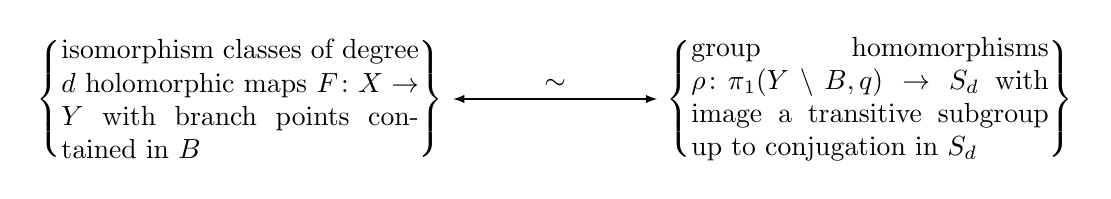
\begin{tikzpicture}[scale=1]
          \node at (-4,0) (maps)
          {
            $
              \left\{
                \begin{minipage}{30ex}
                  isomorphism classes of
                  degree $d$
                  holomorphic maps
                  $F\colon X\to Y$
                  with branch points
                  contained in $B$
                \end{minipage}
              \right\}
            $
          };
          \node at (4,0) (perms)
          {
            $
              \left\{
                \begin{minipage}{30ex}
                  group homomorphisms
                  $\rho\colon\pi_1(Y\sm B, q)\to S_d$
                  with image a transitive subgroup
                  up to conjugation in $S_d$
                \end{minipage}
              \right\}
            $
          };
          % \draw[<->] (maps) to node [above,rotate=-35] {$\sim$} node {} (perms);
          \draw[<->] (maps) to node [above] {$\sim$} node {} (perms);
        \end{tikzpicture}
      \end{center}
    \end{prop}
    If we let $Y = \PP^1$ in Proposition \ref{prop:branchedcoverofriemannsurfaces}
    and $B = \{b_1,\ldots,b_n\}\subseteq\PP^1$ we obtain
    the following correspondence:
    \begin{center}
      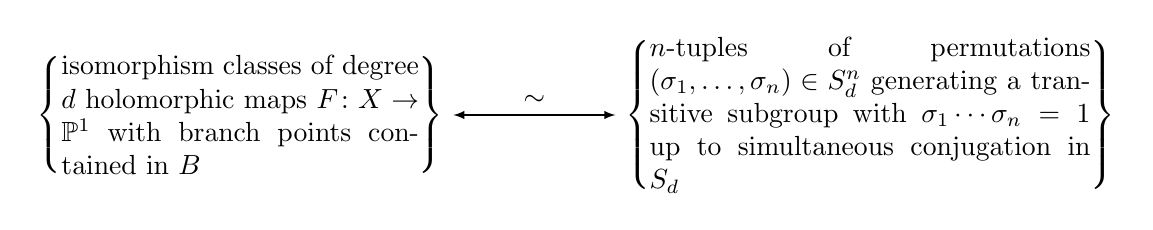
\begin{tikzpicture}[scale=1]
      \label{branchedcoverscorrespondtopermutations}
        \node at (-4,0) (maps)
        {
          $
            \left\{
              \begin{minipage}{30ex}
                isomorphism classes of
                degree $d$
                holomorphic maps
                $F\colon X\to \PP^1$
                with branch points
                contained in $B$
              \end{minipage}
            \right\}
          $
        };
        \node at (4,0) (perms)
        {
          $
            \left\{
              \begin{minipage}{37ex}
                $n$-tuples of permutations
                $(\sigma_1,\ldots,\sigma_n)\in S_d^n$
                generating a transitive subgroup
                with $\sigma_1\cdots\sigma_n=1$
                up to simultaneous conjugation in $S_d$
              \end{minipage}
            \right\}
          $
        };
        % \draw[<->] (maps) to node [above,rotate=-35] {$\sim$} node {} (perms);
        \draw[<->] (maps) to node [above] {$\sim$} node {} (perms);
      \end{tikzpicture}
    \end{center}
    Moreover,
    if $\sigma_i$ has cycle structure $(m_1,\dots,m_k)$,
    then there are $k$ preimages
    $u_1,\dots,u_k$ of $b_i$
    in the cover $F\colon X\to\PP^1$
    with $\mult_{u_j}(F) = m_j$ for all $j$.
    \begin{definition}
      \label{def:belyimapriemannsurface}
      A \defi{Belyi map} is a nonconstant holomorphic map of
      compact connected Riemann surfaces
      $F\colon X\to\PP^1$ with no more than $3$ branch points.
    \end{definition}
    \begin{definition}\label{def:galoiscover}
    \end{definition}
  }
  \section{Algebraic curves}{\label{sec:algebraiccurves}
    Let $K$ be a field isomorphic to the complex numbers,
    the real numbers, a number field, or a finite field.
    Let $\Kal$ denote an algebraic closure of $K$.
    For a detailed treatment see
    \cite[Chapters 1-2]{silverman}.
    %%%%%%%%%%%%AFFINE VARIETIES
    \begin{definition}
      \label{def:affinespace}
      \defi{Affine $n$-space} over $K$ is the
      set of $n$-tuples of elements in $\Kal$
      and denoted $\AA^n(\Kal)$ or $\AA^n$.
      % set of K-rational points of AA^n
    \end{definition}
    We will denote \defi{points} in $\AA^n$ by $P$.
    % Galois action on AA^n
    Let $\Kal[x_1,\dots,x_n]$ be the $n$-variable
    polynomial ring over $\Kal$.
    To each ideal $I\trianglelefteq\Kal[x_1,\dots,x_n]$
    we associate the following subset of $\AA^n$.
    \begin{equation}
      \label{eqn:algebraicset}
      V(I)\colonequals
      \{P\in\AA^n : f(P) = 0 \text{ for all } f\in I\}
    \end{equation}
    \begin{definition}
      \label{def:algebraicset}
      Subsets of $\AA^n$
      of the form $V(I)$ for some ideal $I$
      as in Equation \ref{eqn:algebraicset}
      are called
      \defi{affine algebraic sets}.
    \end{definition}
    Let $V$ be an affine algebraic set.
    To such a set we can associate
    the following ideal of $\Kal[x_1,\dots,x_n]$.
    \begin{equation}
      \label{eqn:idealofalgebraicset}
      I(V)\colonequals
      \{f\in\Kal[x_1,\dots,x_n]: f(P)=0 \text{ for all }f\in I\}.
    \end{equation}
    \begin{definition}
      \label{def:definedoverK}
      Let $\AA^n(K)$ denote the set of
      \defi{$K$-rational points} of $\AA^n$ defined by
      \[
        \AA^n(K)\colonequals
        \{(x_1,\dots,x_n)\in\AA^n : x_i\in K\}.
      \]
      Let $V$ be an algebraic set.
      We say $V$ is
      \defi{defined over $K$}
      if $I(V)$ can be generated by
      polynomials in $K[x_1,\dots,x_n]$.
      For such $V$ we can define the
      \defi{$K$-rational points of $V$} by
      \[
        V(K)\colonequals
        V\cap\AA^n(K).
      \]
    \end{definition}
    Let $G_K = \Gal(\Kal/K)$.
    Another way to characterize $V(K)$ is
    the points fixed under the action of $G_K$:
    \begin{equation}
      \label{eqn:galoisactiononV}
      V(K) =
      \{P\in V : P^\sigma = P\text{ for all }\sigma\in G_K\}
    \end{equation}
    \begin{definition}
      \label{def:affinevariety}
      An affine algebraic set $V$ is called
      an \defi{affine variety}
      if $I(V)\trianglelefteq\Kal[x_1,\dots,x_n]$ is a prime ideal.
    \end{definition}
    If an affine algebraic set $V$ is defined over $K$,
    then $V$ is an affine variety if
    $I(V)\trianglelefteq K[x_1,\dots,x_n]$
    is a prime ideal.
    \begin{definition}
      \label{def:coordinateringfunctionfield}
      Let $V$ be an affine variety defined over $K$.
      We define the
      \defi{affine coordinate ring}
      by
      \[
        K[V]
        \colonequals
        \frac{
          K[x_1,\dots,x_n]
        }{
        I(V)
        }
      \]
      and the
      \defi{function field of $V$}
      by the field of fractions of $K[V]$
      denoted $K(V)$.
      We can similarly define this construction
      for $\Kal[V]$ and $\Kal(V)$.
    \end{definition}
    \begin{definition}
      \label{def:dimension}
      The \defi{dimension}
      of an affine variety $V$
      is the transcendence degree of the field extension
      $\Kal(V)$ over $\Kal$.
    \end{definition}
    % \begin{definition}
    %   \label{def:nonsingular}
    %   Let $V$ be an affine variety of dimension $d$,
    %   let $P\in V$,
    %   and $I(V)$ generated by
    %   $\{f_1,\dots,f_m\}$.
    %   We say $V$ is \defi{nonsingular at $P$}
    %   if the $m\times n$ matrix of partial
    %   derivatives
    %   whose $(i,j)$-entry is
    %   \[
    %     \frac{\partial f_i}{\partial x_j}
    %   \]
    %   has rank $n-d$.
    % \end{definition}
    \begin{definition}
      \label{def:nonsingular}
      Let $V$ be a variety of dimension $d$
      and $P\in V$.
      Consider the maximal ideal
      \[
        M_P\colonequals
        \{f\in\Kal[x_1,\dots,x_n]:f(P)=0\}.
      \]
      The quotient $M_P/M_P^2$ is a finite dimensional
      vector space over $\Kal$.
      We say $P$ is \defi{nonsingular}
      if the dimension of $M_P/M_P^2$ as
      a vector space over $\Kal$
      is equal to $d$.
    \end{definition}
    \begin{definition}
      \label{def:localringatP}
      Let $V$ be an affine variety
      and $P\in V$.
      The \defi{ring of regular functions on $V$ at $P$}
      is defined to be the localization
      of $\Kal[V]$ at the maximal ideal $M_P$
      (denoted $\Kal[V]_P$).
      More explicitly we have
      \[
        \Kal[V]_P
        \colonequals
        \Kal[V]_{M_P}
        =
        \{f/g\in\Kal[V]:g(P)\neq 0\}
      \]
      so that
      the elements of
      $\Kal[V]_P$
      are well-defined
      as functions on $V$.
    \end{definition}
    %%%%%%%%%%%%PROJECTIVE VARIETIES
    \begin{definition}
      \label{def:projectivespace}
      \defi{Projective $n$-space}
      over $K$ is denoted by $\PP^n(\Kal)$
      or $\PP^n$
      and is defined to be
      \[
        \PP^n\colonequals
        \{(x_0,\dots,x_{n})\in\AA^{n+1}:\text{ not all $x_i=0$ }\}/\sim
      \]
      where
      $(x_0,\dots,x_n)\sim(x_0',\dots,x_n')$
      if there exists $\lambda\in(\Kal)^\times$ with
      $x_i=\lambda y_i$ for all $i\in \{0,\dots,n\}$.
      The equivalence class of $(x_0,\dots,x_n)\in\AA^{n+1}$
      with respect to $\sim$ is denoted by
      $[x_0,\dots,x_n]$ or $[x_0:\cdots:x_n]$.
      We call these $x_i$
      \defi{homogeneous coordinates}
      of the point in $\PP^n$.
      As in the affine case,
      we define the
      \defi{$K$-rational points} of $\PP^n$
      to be
      \[
        \PP^n(K)\colonequals
        \{[x_0,\dots,x_n]\in\PP^n:x_i\in K \text{ for all } i\}.
      \]
    \end{definition}
    \begin{definition}
      \label{def:minimalfieldofdefinitionPPn}
      Let $P\in\PP^n$ with homogeneous coordinates
      $[x_0,\dots,x_n]$.
      The \defi{minimal field of definition of $P$ over $K$}
      is
      \[
        K(P)\colonequals
        K(x_0/x_i,\dots,x_n/x_i)
      \]
      for any $i\in \{0,\dots,n\}$.
    \end{definition}
    $\PP^n(K)$ is the set of $P\in\PP^n$
    fixed by the action of $G_K$.
    On the other hand,
    $K(P)$ is the fixed field of the
    subgroup
    $\{\sigma\in G_K: P = P^\sigma\}$.
    \begin{definition}
      \label{def:homogeneousideal}
      An ideal $I\trianglelefteq\Kal[x_0,\dots,x_n]$
      is \defi{homogeneous}
      if it can be generated by homogeneous polynomials.
      To a homogeneous ideal $I$ we can associate a subset of
      $\PP^n$ as follows.
      \[
        V(I)\colonequals
        \{P\in\PP^n : f(P)=0\text{ for all homogeneous $f\in\Kal[x_0,\dots,x_n]$ }\}
      \]
      A \defi{projective algebraic set}
      is a subset of $\PP^n$ which is $V(I)$
      for some homogeneous ideal $I$.
    \end{definition}
    To any projective algebraic set $V$,
    we can associate a homogeneous ideal $I(V)$ defined by
    \begin{equation}
      \label{eqn:projectivealgebraicsetideal}
      I(V)
      \colonequals
      \{f\in\Kal[x_0,\dots,x_n]:f \text{ is homogeneous and }f(P) = 0\text{ for all $P\in V$ }\}
    \end{equation}
    % \begin{theorem}\label{thm:curvesandfunctionfields}
    %   \mm{correspondence curves and function fields}
    % \end{theorem}
    % \begin{definition}
    %   Let $K\subseteq\CC$ be a field.
    %   A \defi{branched cover of algebraic curves over $K$}
    %   is a finite map of curves
    %   $\phi\colon X\to\PP^1$ defined over $K$.
    % \end{definition}
    % \mm{enough to define good curves and function fields}
  }
  \section{Riemann's existence theorem}{\label{sec:riemannsexistence}
    Riemann surfaces are defined in Section \ref{sec:riemannsurfaces}.
    Algebraic curves are defined in Section \ref{sec:algebraiccurves}.
    Here in Section \ref{sec:riemannsexistence}
    we establish the connection between these objects over the complex numbers.
    \par
    Let $X$ be an algebraic curve over $\CC$.
    Let $\CC(t)$ denote the function field of $\PP^1$.
    By Theorem \ref{thm:curvesandfunctionfields},
    $X$ corresponds to a finite extension $L\colonequals\CC(X)$
    over $\CC(t)$.
    Let $\alpha$ be a primitive element of $L/\CC(t)$.
    Then there exists a polynomial
    \begin{equation}
      \label{eqn:minpoly}
      f(x,t) = a_0(t)+a_1(t)x+a_2(t)x^2+\cdots+a_n(t)x^n\in\CC(t)[x]
    \end{equation}
    where $f(\alpha,t) = 0$ and (after possibly clearing denominators)
    $a_i(t) \in\CC[t]$.
    The polynomial $f$ in Equation \ref{eqn:minpoly}
    defines a Riemann surface $X'$
    as a branched cover of $\PP^1$
    with branch points
    \[
      S \colonequals\left\{t_0\in\CC : f(x,t_0) \text{ has repeated roots }\right\}.
    \]
    Here $x$ can be viewed as a meromorphic function on $X'$
    and we can identify the field of meromorphic functions on $X'$
    with $L$.
    This explains how we obtain a Riemann surface from an algebraic curve.
    \par
    Suppose instead we start with a compact Riemann surface $X$.
    Can we reverse the above process to construct an algebraic curve?
    The crucial part of this process is proving that
    there exists a meromorphic function on $X$ that realizes $X$
    as a branched cover of $\PP^1$
    (see Theorem \ref{thm:riemannsexistence} below).
    Given the existence of such a function,
    the field of meromorphic functions on $X$ is then realized
    as a finite extension of the meromorphic functions on $\PP^1$.
    Finally,
    by Theorem \ref{thm:curvesandfunctionfields},
    this corresponds to an algebraic curve.
    The existence of such a function
    is given by
    Theorem \ref{thm:riemannsexistence}
    (Riemann's existence theorem).
    \begin{theorem}\label{thm:riemannsexistence}
      Let $X$ be a compact Riemann surface.
      Then there exists a meromorphic function on $X$
      that separates points.
      That is, for any set of distinct points
      $\{x_1,\dots,x_n\}\subset X$
      and any set of distinct points
      $\{t_1,\dots,t_n\}\subset\PP^1$
      there exists a meromorphic function $f$
      on $X$ such that $f(x_i) = t_i$ for all $i$.
    \end{theorem}
    \mm{todo: more details...other formulations}
  }
  \section{Belyi's theorem}{\label{sec:belyistheorem}
    In Sections
    \ref{sec:riemannsufraces}, \ref{sec:algebraiccurves},
    and \ref{sec:riemannsexistence}
    we established the equivalence between
    compact Riemann surfaces and algebraic curves over $\CC$.
    This was done, in part,
    using branched covers.
    It turns out that branched covers are the key
    to descending from the transcendental world to
    the number-theoretic world in the following sense.
    \begin{theorem}[Belyi's theorem \cite{belyi}]\label{thm:belyistheorem}
      An algebraic curve $X$ over $\CC$ can be defined over a number field
      if and only if there exists a branched cover
      $\phi\colon X\to\PP^1$ unramified outside
      $\{0,1,\infty\}$.
    \end{theorem}
    These remarkable covers are the main focus of this work.
  }
  \section{Belyi maps and Galois Belyi maps}{\label{sec:belyimaps}
    We now set up the framework to discuss
    the main mathematical objects of interest in this work.
    \begin{definition}\label{def:belyimap}
      A \defi{Belyi map}
      is a branched cover
      of algebraic curves over $\CC$
      (equivalently of Riemann surfaces)
      $\phi\colon X \to \PP^1$
      that is
      unramified outside
      $\{0,1,\infty\}$.
    \end{definition}
    \begin{definition}\label{def:belyiiso}
      Two Belyi maps
      $\phi\colon X\to\PP^1$ and
      $\phi'\colon X'\to\PP^1$
      are \defi{isomorphic}
      if there exists an isomorphism
      between $X$ and $X'$
      such that the diagram in Figure
      \ref{fig:belyiiso}
      commutes.
      If instead we only insist that the isomorphism
      makes the diagram in Figure
      \ref{fig:belyilax} commute,
      then we say that $\phi$ and $\phi'$
      are \defi{lax isomorphic}.
      \begin{figure}[ht]
        \begin{center}
          \begin{tikzcd}
            X\arrow{rr}{\sim}\arrow{dr}[swap]{\phi}&&X'\arrow{dl}{\phi'}\\
                                                   &\PP^1
          \end{tikzcd}
        \end{center}
        \caption{Belyi map isomorphism}
        \label{fig:belyiiso}
      \end{figure}
      \begin{figure}[ht]
        \begin{center}
          \begin{tikzcd}
            X\arrow{r}{\sim}\arrow{d}[swap]{\phi}&X'\arrow{d}{\phi'}\\
            \PP^1\arrow{r}{\sim}&\PP^1
          \end{tikzcd}
        \end{center}
        \caption{Belyi map lax isomorphism}
        \label{fig:belyilax}
      \end{figure}
    \end{definition}
    \begin{definition}\label{def:galoisbelyi}
      A Belyi map $\phi\colon X\to\PP^1$
      is \defi{Galois}
      if it is Galois as a cover
      (see Definition \ref{def:galoiscover}).
      A curve $X$ that admits a Galois Belyi map
      is called a \defi{Galois Belyi curve}.
    \end{definition}
    \begin{prop}\label{prop:galoiscover}
      Let $\phi\colon X\to\PP^1$ be a Galois Belyi map
      and let $\CC(X)$ be the function field of $X$.
      Then the field extension
      $\CC(X)/\CC(\PP^1)$ is Galois.
    \end{prop}
    \begin{proof}
    \end{proof}
    \begin{definition}\label{def:ramificationtype}
      The ramification
      of a degree $d$ Belyi map $\phi$
      can be encoded with $3$ partitions of $d$
      denoted $(\lambda_0,\lambda_1,\lambda_\infty)$.
      We call this triple of partitions
      the \defi{ramification type} of $\phi$.
      When $\phi$ is Galois,
      according to Lemma \ref{lem:regular},
      the ramification type of $\phi$ can more simply be encoded by
      a triple of integers $(a,b,c)\in\ZZ_{\geq 1}^3$.
    \end{definition}
    Let $\phi\colon X\to\PP^1$ be a Belyi map of degree $d$.
    Once we label the sheets of the cover
    and pick a basepoint $\star\not\in\{0,1,\infty\}$,
    we obtain a homomorphism
    \begin{equation}\label{eqn:monodromy}
      h\colon\pi_1(\PP^1\setminus\{0,1,\infty\},\star)\to S_d
    \end{equation}
    by lifting paths around the branch points of $\phi$.
    \begin{definition}\label{def:monodromy}
      The image of $h$ in Equation \ref{eqn:monodromy}
      is the \defi{monodromy group} of $\phi$
      denoted $\Mon(\phi)$.
      When $\phi$ is a Galois Belyi map,
      we can identify $\Mon(\phi)$
      as the Galois group
      $\Gal(\CC(X)/\CC(\PP^1))$.
      For this reason,
      we may also write $\Gal(\phi)$
      to denote $\Mon(\phi)$ when $\phi$
      is Galois.
    \end{definition}
    \mm{todo: any propositions about monodromy groups can go here}
    \begin{definition}\label{def:Gbelyi}
      A \defi{$G$-Galois Belyi map}
      is a Galois Belyi map
      $\phi\colon X\to\PP^1$
      with monodromy group $G$
      equipped with an isomorphism
      \[
        i\colon G\stackrel{\sim}{\to}\Mon(\phi)\leq\Aut(X).
      \]
      An \defi{isomorphism of $G$-Galois Belyi maps}
      $(\phi\colon X\to\PP^1, i\colon G\to\Mon(\phi))$
      and
      $(\phi'\colon X'\to\PP^1, i'\colon G\to\Mon(\phi)$
      is an isomorphism $h\colon X\stackrel{\sim}{\to} X'$ such that
      for all $g\in G$
      the diagram in
      Figure \ref{fig:Gbelyiiso} commutes.
      \begin{figure}[ht]
        \begin{center}
          \begin{tikzcd}
            X\arrow{rr}{h}\arrow{d}[swap]{i(g)}&&X'\arrow{d}{i'(g)}\\
            X\arrow{rr}{h}\arrow{dr}[swap]{\phi}&&X'\arrow{dl}{\phi'}\\
                                                   &\PP^1
          \end{tikzcd}
        \end{center}
        \caption{$G$-Galois Belyi map isomorphism}
        \label{fig:Gbelyiiso}
      \end{figure}
      \begin{prop}\label{prop:Gauts}
        \mm{\cite[Prop. 3.6 ish]{triangles}}
      \end{prop}
    \end{definition}
  }
  \section{Permutation triples and passports}{\label{sec:passports}
    % A \defi{(nice) curve} over $K$ is
    % a smooth, projective, geometrically connected (irreducible) scheme of finite
    % type over $K$ that is pure of dimension $1$.
    % After extension to $\CC$, a curve
    % may be thought of as a compact, connected Riemann surface.  A \defi{Belyi map}
    % over $K$ is a finite morphism $\phi\colon X \to \PP^1$ over $K$ that is
    % unramified outside $\{0,1,\infty\}$; we will sometimes write $(X,\phi)$ when we
    % want to pay special attention to the source curve $X$.  Two Belyi maps
    % $\phi,\phi'$ are \defi{isomorphic} if there is an isomorphism $\iota\colon X
    % \xrightarrow{\sim} X'$ of curves such that $\phi'\iota=\phi$.
    % Let $\phi\colon X\to\PP^1$ be a Belyi map over $\overline{\QQ}$ of degree
    % $d \in \ZZ_{\geq 1}$.
    % The \defi{monodromy group} of $\phi$ is the Galois group
    % $\Mon(\phi) \colonequals \Gal(\CC(X)\,|\,\CC(\PP^1)) \leq S_d$ of the
    % corresponding extension of function fields (understood as the action of the
    % automorphism group of the normal closure); the group $\Mon(\phi)$ may also be
    % obtained by lifting paths around $0,1,\infty$ to $X$.
    \begin{definition}
      \label{def:permutationtriple}
      A \defi{permutation triple} of degree $d \in \ZZ_{\geq 1}$ is a tuple $\sigma =
      (\sigma_0,\sigma_1,\sigma_\infty)\in S_d^3$ such that $\sigma_\infty \sigma_1
      \sigma_0 = 1$.
      A permutation triple is \defi{transitive} if the subgroup
      $\langle \sigma \rangle \leq S_d$ generated by $\sigma$ is transitive.
      We say
      that two permutation triples $\sigma,\sigma'$ are \defi{simultaneously
      conjugate} if there exists $\tau\in S_d$ such that
      \begin{equation}\label{eqn:simconj}
        \sigma^\tau \colonequals
        (\tau^{-1}\sigma_0\tau, \tau^{-1}\sigma_1\tau, \tau^{-1}\sigma_\infty\tau)
        = \left(\sigma'_0,\sigma'_1,\sigma'_\infty\right)
        = \sigma'.
      \end{equation}
      An \defi{automorphism} of a permutation triple $\sigma$ is an element of $S_d$ that
      simultaneously conjugates $\sigma$ to itself, i.e.,
      $\Aut(\sigma)=Z_{S_d}(\langle \sigma \rangle)$, the centralizer inside $S_d$.
    \end{definition}
    \begin{lemma}
      \label{lem:simulisom}
      The set of transitive permutation triples of degree $d$ up to simultaneous
      conjugation is in bijection with the set of Belyi maps of degree $d$ up to
      isomorphism.
    \end{lemma}
    \begin{proof}
      The correspondence is via monodromy \cite[Lemma 1.1]{KMSV}; in particular,
      the monodromy group of a Belyi map is (conjugate in $S_d$ to) the group
      generated by~$\sigma$.
    \end{proof}
    The group $G_\QQ\colonequals\Gal(\QQal/ \QQ)$ acts on Belyi maps by acting on the
    coefficients of a set of defining equations; under the bijection of Lemma
    \ref{lem:simulisom}, it thereby acts on the set of transitive permutation
    triples, but this action is rather mysterious.
    We can cut this action down to size by identifying some basic invariants, as
    follows.
    \begin{definition}
      \label{def:passport}
      A \defi{passport} consists of the data $\mathcal{P}=(g,G,\lambda)$
      where $g \geq 0$ is an integer, $G \leq S_d$ is a transitive subgroup, and
      $\lambda=(\lambda_0,\lambda_1,\lambda_\infty)$ is a tuple of partitions
      $\lambda_s$ of $d$ for $s=0,1,\infty$.
      These partitions will be also be
      thought of as a tuple of conjugacy classes $C=(C_0,C_1,C_\infty)$ by cycle
      type, so we will also write passports as $(g,G,C)$.
    \end{definition}
    \begin{definition}
      \label{def:passportofbelyimap}
      The \defi{passport} of a
      Belyi map $\phi\colon X \to \PP^1$ is $(g(X),\Mon(\phi),
      (\lambda_0,\lambda_1,\lambda_\infty))$,
      where $g(X)$ is the genus of $X$ and
      $\lambda_s$ is the partition of $d$ obtained by the ramification degrees above
      $s=0,1,\infty$, respectively.
    \end{definition}
    \begin{definition}
      \label{def:passportofpermutationtriple}
      The \defi{passport} of a transitive
      permutation triple $\sigma$ is
      $(g(\sigma),\langle \sigma \rangle, \lambda(\sigma))$,
      where (by Riemann--Hurwitz)
      \begin{equation}\label{eqn:riemannhurwitzfortriples}
        g(\sigma) \colonequals 1-d+(e(\sigma_0)+e(\sigma_1)+e(\sigma_\infty))/2
      \end{equation}
      and $e$ is the index of a permutation ($d$ minus the number of orbits), and
      $\lambda(\sigma)$ is the cycle type of $\sigma_s$ for $s=0,1,\infty$.
    \end{definition}
    \begin{definition}
      \label{def:passportsize}
      The
      \defi{size} of a passport $\mathcal{P}$ is the number of simultaneous conjugacy
      classes (as in \ref{eqn:simconj}) of (necessarily transitive) permutation
      triples $\sigma$ with passport $\mathcal{P}$.
    \end{definition}
    The action of $G_\QQ$ on Belyi maps preserves passports.
    Therefore, after computing equations for all Belyi maps with a given
    passport, we can try to identify the Galois orbits of this action.
    \begin{definition}
      \label{def:reduciblepassport}
      We say a passport is \defi{irreducible} if it has one
      $G_\QQ$-orbit and
      \defi{reducible} otherwise.
    \end{definition}
  }
  \section{Triangle groups}{\label{sec:trianglegroups}
    \begin{definition}
      \label{def:geometrytype}
      Let $(a,b,c)\in\ZZ_{\geq 1}^3$.
      If $1\in(a,b,c)$, then we say the triple is \defi{degenerate}.
      Otherwise, we call the triple
      \defi{spherical},
      \defi{Euclidean},
      or \defi{hyperbolic}
      according to whether the value of
      \begin{equation}
        \label{eqn:eulerchar}
        \chi(a,b,c) = 1-\frac{1}{a}-\frac{1}{b}-\frac{1}{c}
      \end{equation}
      is negative, zero, or positive.
      We call this the \defi{geometry type}
      of the triple.
      We associate the \defi{geometry}
      \begin{equation}
        \label{eqn:geometrytype}
        H=
        \begin{cases}
          \PP^1&\chi(a,b,c)<0\\
          \CC&\chi(a,b,c)=0\\
          \mathfrak{H}&\chi(a,b,c)<0
        \end{cases}
      \end{equation}
      where $\mathfrak{H}$ denotes the complex upper half-plane.
    \end{definition}
    \begin{definition}
      \label{def:trianglegroup}
      For each triple $(a,b,c)$ in Definition \ref{def:geometrytype}
      we define the \defi{triangle group}
      \begin{equation}
        \label{eqn:trianglegroup}
        \Delta(a,b,c)
        =
        \langle
        \delta_a, \delta_b, \delta_c |
        \delta_a^a=\delta_b^b=\delta_c^c=\delta_c\delta_b\delta_a=1
        \rangle
      \end{equation}
      The \defi{geometry type}
      of a triangle group $\Delta(a,b,c)$
      is the geometry type of the triple $(a,b,c)$.
    \end{definition}
    \begin{definition}\label{def:geometrytypeofbelyimap}
      The \defi{geometry type} of a Galois Belyi map
      with ramification type $(a,b,c)$
      is the geometry type of $(a,b,c)$.
    \end{definition}
    \begin{definition}\label{def:geometrytypeofpermutationtriple}
      Let $\sigma=(\sigma_0,\sigma_1,\sigma_\infty)$ be a transitive permutation triple.
      Let $a,b,c$ be the orders of
      $\sigma_0,\sigma_1,\sigma_\infty$ respectively.
      The \defi{geometry type} of $\sigma$
      is the geometry type of $(a,b,c)$.
    \end{definition}
    The connection between Belyi maps and triangle groups
    of various geometry types is explained by Lemma
    \ref{lem:belyimapsandtrianglegroups}.
    \begin{lemma}
      \label{lem:belyimapsandtrianglegroups}
      The set of isomorphism classes of of degree $d$
      Belyi maps with ramification type $(a,b,c)$
      is in bijection with the set of
      index $d$ subgroups
      $\Gamma\leq\Delta(a,b,c)$
      up to isomorphism.
    \end{lemma}
    \begin{proof}
      See \cite{KMSV} for a detailed discussion.
    \end{proof}
  }
  \section{Background results on Belyi maps}{\label{sec:backgroundresults}
    \begin{theorem}\label{thm:bigbijection}
      \mm{big bijection}
    \end{theorem}
    \begin{prop}\label{prop:galoisaction}
      \mm{Galois action on Belyi maps}
    \end{prop}
    \begin{prop}\label{prop:galoiscorrespondence}
      Galois correspondence of Belyi maps
    \end{prop}
    \begin{proof}
    \end{proof}
    \mm{\cite[1.6, 1.7]{SV}}
  }
  \section{Fields of moduli and fields of definition}{\label{sec:fieldsofmodulifieldsofdefinition}
    Let $\Aut(\CC)$ denote the field automorphisms of $\CC$.
    \begin{definition}
      \label{def:fieldofmoduli}
      Let $X$ be an algebraic curve over $\CC$.
      The \defi{field of moduli} of $X$ is the fixed field of the
      field automorphisms
      \[
        \{\tau\in\Aut(\CC) : X^\tau\cong X\}
      \]
      where $\tau\in\Aut(\CC)$ acts on the defining equations of $X$.
      Denote this field as $M(X)$.
    \end{definition}
    \begin{definition}
      \label{def:fieldofmodulibelyimap}
      Let $\phi\colon X\to\PP^1$ be a Belyi map.
      The \defi{field of moduli} of $\phi$ is the fixed field of the
      field automorphisms
      \[
        \{\tau\in\Aut(\CC) : \phi^\tau\cong \phi\}
      \]
      where $\tau\in\Aut(\CC)$ acts on the defining equations of $\phi$
      and isomorphism is determined by
      Definition \ref{def:belyiiso}.
      Denote this field as $M(\phi)$.
    \end{definition}
    \begin{definition}
      \label{def:fieldofmoduliGbelyimap}
      Let $\phi\colon X\to\PP^1$ be a $G$-Galois Belyi map.
      The \defi{field of moduli} of $\phi$ is the fixed field of the
      field automorphisms
      \[
        \{\tau\in\Aut(\CC) : \phi^\tau\cong \phi\}
      \]
      where $\tau\in\Aut(\CC)$ acts on the defining equations of $\phi$
      and isomorphism is determined by
      Definition \ref{def:Gbelyi}.
      Denote this field as $M(\phi)$.
    \end{definition}
    \begin{theorem}\label{thm:fieldofmoduli}
      Let $\phi:X\to\PP^1$ be a Belyi map
      with passport $\mathcal{P}$.
      Then the degree of the field of moduli of $\phi$
      is bounded by the size of $\mathcal{P}$.
    \end{theorem}
    \begin{proof}
      \cite{SV}
    \end{proof}
    \begin{definition}
      \label{def:fieldofdefinition}
      Let $\phi\colon X\to\PP^1$ be a Belyi map.
      A number field $K$ is a
      \defi{field of definition} for $\phi$
      if $\phi$ and $X$ can be defined
      with equations over $K$.
      If $K$ is a field of definition for $\phi$
      we say $\phi$ is \defi{defined over} $K$.
    \end{definition}
    \begin{theorem}
      \label{thm:galoisbelyimapoverfieldofmoduli}
      A Galois Belyi map is defined over
      its field of moduli.
    \end{theorem}
    \begin{proof}
      \cite[Lemma 4.1]{triangles}
    \end{proof}
  }
}
\chapter{Group theory}{\label{chapter:grouptheory}
  In this chapter we discuss results on the groups
  that arise as monodromy groups
  of the Belyi maps we are interested in.
  \section{$2$-groups}{\label{sec:twogroups}
    % def, center, exact sequence, group coho, cosets
    % examples, families: gen dihedral, gen quats, etc
    \mm{references \cite{DF}\ldots}
    Let $G$ be a finite group.
    Denote the \defi{centralizer} and
    \defi{normalizer} of a subet $S\subseteq G$
    by $C_G(S)$ and $N_G(S)$ respectively.
    Let $G$ act on a set $X$.
    For $x\in X$
    denote the \defi{stabilizer of $x$} by
    $\stab_x(G)$
    and the \defi{orbit of $x$} by
    $\orb_x(G)$.
    \begin{definition}
      \label{def:pgroup}
      Let $p$ be a rational prime.
      A finite group $G$ is a
      \defi{$p$-group}
      if the cardinality of $G$
      is a power of $p$.
    \end{definition}
    \begin{lemma}
      \label{lem:pgrouphasacenter}
      The center of a nontrivial $p$-group is nontrivial.
    \end{lemma}
    \begin{proof}
      Let $G$ be a $p$-group acting on itself by conjugation.
      Note that for $g\in G$ we have
      $C_G(g)=\stab_g(G)=N_G(\{g\})$,
      and
      $Z(G)=\cap_g C_G(g)$.
      Let
      $C_g\colonequals\orb_g(G)$
      denote the conjugacy class of $g\in G$.
      Then $\#C_g = [G:C_G(g)]$ for every $g$.
      Partitioning $G$ into conjugacy classes we obtain
      \begin{equation}\label{eqn:classequation}
        \#G =
        \#Z(G)+\sum_{i=1}^r[G:C_G(g_i)]
      \end{equation}
      where $\{g_1,\dots,g_r\}$ is a set of representatives of distinct
      conjugacy classes not contained in $Z(G)$.
      Since $g_i\not\in Z(G)$, $p$ divides $[G:C_G(g_i)]$ for every $i$.
      Then Equation \ref{eqn:classequation} implies $p$ divides
      $\#Z(G)$.
    \end{proof}
    \begin{lemma}
      \label{lem:conjugacyinsubgroups}
      Let $H$ be a normal subgroup of a $p$-group $G$.
      Let $C$ be a conjugacy class of $G$.
      Then either $C\subseteq H$ or $C\cap H = \emptyset$.
    \end{lemma}
    \begin{proof}
      Suppose $a\in C\cap H$.
      Let $x\in C$.
      Then there exists $g\in G$ so that
      $x = gag^{-1}$.
      But $a\in H$ and $H$ is normal,
      so $x=gag^{-1}\in H$.
      Thus $C\subseteq H$.
    \end{proof}
    \begin{lemma}
      \label{lem:normalimpliescentralintersect}
      Let $G$ be a $p$-group.
      Let $H$ be a nontrivial normal subgroup of $G$.
      Then $H$ intersects the center $Z(G)$ nontrivially.
    \end{lemma}
    \begin{proof}
      Let $\{g_1,\dots,g_r\}$ be a set of representatives of the
      $r$ distinct conjugacy classes (denoted $C_i$)
      of $G$ with $\#C_i\ge 2$.
      We will use Equation \ref{eqn:classequation}
      for the subgroup $H$, so
      by Lemma \ref{lem:conjugacyinsubgroups}
      we may assume all $g_i\in H$.
      The conjugacy classes of size $1$ are contained in the center $Z(G)$
      and as in Equation \ref{eqn:classequation} we
      can write
      \begin{equation}
        \label{eqn:classequationsubgroup}
        \#H = \#(H\cap Z(G))+
        \sum_{i=1}^r[G:C_G(g_i)].
      \end{equation}
      As in the proof of
      Lemma \ref{lem:pgrouphasacenter}
      we see that $p$ divides $\#(H\cap Z(G))$.
    \end{proof}
    \begin{corr}
      \label{cor:normalcentral}
      Let $H$ be a normal subgroup of order $p$ of a $p$-group $G$.
      Then $H$ is central.
    \end{corr}
    \begin{proof}
      By Lemma \ref{lem:normalimpliescentralintersect},
      $H\cap Z(G)$ is a nontrivial subgroup of $G$
      or order at least $p$.
      Since $\#H=p$ this tells us
      $H=H\cap Z(G)$.
      In particular,
      $H$ is contained in $Z(G)$.
    \end{proof}
    \begin{lemma}
      \label{lem:normalsubgroupsofallorders}
      Let $H$ be a normal subgroup of a $p$-group $G$.
      Let $\#G=p^\alpha$.
      Then $H$ contains a subgroup $H_\beta$ of order $p^\beta$
      for every divisor $p^\beta$ of $\#H$
      with the property that
      $H_\beta$ is normal in $G$ for every $\beta$.
    \end{lemma}
    \begin{proof}
    \end{proof}
    \begin{corr}
      \label{cor:normalsubgroupsofallorders}
    \end{corr}
    \begin{lemma}
      \label{lem:propersubgroupcontainedinnormalizer}
      A proper subgroup $H$ of a $p$-group $G$
      is contained in its normalizer $N_G(H)$.
    \end{lemma}
    \begin{proof}
    \end{proof}
    \begin{lemma}
      \label{lem:maximalsubgroup}
      Every maximal subgroup $H$ of a $p$-group $G$
      has $[G:H]=p$ and $H\trianglelefteq G$.
    \end{lemma}
    \begin{proof}
    \end{proof}
    \begin{definition}
      \label{def:uppercentralseries}
      Let $G$ be a finite group.
      We define a sequence of subgroups of $G$ iteratively as follows.
      Let $Z_0(G) = \{1\}$
      and let $Z_1(G) = Z(G)$.
      For $i\geq 2$ consider
      the map
      \[
        \pi\colon G\to G/Z_i(G),
      \]
      and define $Z_{i+1}(G)$ to be the preimage of the center of $G/Z_i(G)$ under $\pi$
      as follows.
      \[
        Z_{i+1}(G)\colonequals\pi^{-1}
        \left(Z\left(\frac{G}{Z_i(G)}\right)\right)
      \]
      Continuing this process produces a sequence of
      characteristic subgroups of $G$
      \[
        Z_0(G)\trianglelefteq Z_1(G)\trianglelefteq\cdots\trianglelefteq Z_{i}(G)\trianglelefteq\cdots
      \]
      called the \defi{upper central series} of $G$.
    \end{definition}
    \begin{definition}
      \label{def:lowercentralseries}
      For $x,y\in G$ a finite group,
      define the \defi{commutator of $x$ and $y$}
      by
      $[x,y]\colonequals x^{-1}y^{-1}xy$.
      For subgroups $H,K$ of $G$ define
      $[H,K]\colonequals\langle[h,k]:h\in H\text{ and }k\in K\rangle$.
      We define the \defi{lower central series} of $G$ iteratively as follows.
      Let $G^0=G$,
      let $G^1 = [G,G]$,
      and for $i\geq 1$ define
      $G^{i+1}=[G,G^i]$.
    \end{definition}
    \begin{definition}
      \label{def:nilpotentgroup}
      A finite group $G$ is \defi{nilpotent}
      if the upper central series
      \[
        Z_0(G)\trianglelefteq Z_1(G)\trianglelefteq\cdots\trianglelefteq Z_{i}(G)\trianglelefteq\cdots
      \]
      has $Z_c(G) = G$ for some nonnegative integer $c$.
      The integer $c$ is called the \defi{nilpotency class} of
      the nilpotent group $G$.
    \end{definition}
    \begin{lemma}
      \label{lem:upperlowernilpotent}
      % Thm 8 chapter 6.1 DF
      A finite group $G$ is nilpotent if and only if
      $G^c=\{1\}$ for some nonnegative integer $c$.
      Moreover,
      the smallest $c$ such that $G^c=\{1\}$
      is the nilpotency class of $G$ and
      \[
        Z_i(G)\leq G^{c-i-1}\leq Z_{i+1}(G)
      \]
      for all $i\in \{0,1,\dots,c-1\}$.
    \end{lemma}
    \begin{lemma}
      % Prop 2 chapter 6.1 DF
      A $p$-group of order $p^\alpha$ is nilpotent with nilpotency class
      at most $\alpha-1$.
    \end{lemma}
    \begin{proof}
    \end{proof}
    \begin{lemma}
      % Prop 7 chapter 6.1 DF
      A finite group is nilpotent if and only if
      every maximal subgroup is normal.
    \end{lemma}
    \begin{proof}
    \end{proof}
    \begin{definition}
      \label{def:frattinisubgroup}
      For a group $G$,
      define $\Phi(G)$
      to be the intersection of all maximal subgroups of $G$.
      $\Phi(G)$ is called the
      \defi{Frattini subgroup of $G$}.
    \end{definition}
    % frattini quotient and generators
  }
  \section{Examples of $2$-groups}{\label{sec:twogroupexamples}
    % examples, families: gen dihedral, gen quats, etc
    % In this section we discuss some special families of $2$-groups.
    % maybe these show up later in the "proof of the conjecture"
    In this section we describe several families of
    nonabelian $2$-groups
    that we reference in the partial proof
    of Conjecture \ref{conj:refinedpassportsizeone}.
    The first examples are $2$-groups
    with a cyclic index $2$ subgroup.
    According to
    \cite[Theorem 1.2]{berkovich1},
    these groups all have a center of order $2$,
    abelianization of order $4$,
    and maximal nilpotency class.
    % \begin{example}
      % \label{exm:cyclic}
      % For $n\geq 1$ define
      % $C_{2^n}$ to be the \defi{cyclic group of order $2^n$}
      % with presentation
      % \[
      %   \left\langle
      %     a\mid
      %     a^{2^n}=1
      %   \right\rangle.
      % \]
      % % \begin{itemize}
      % %   \item
      % % \end{itemize}
    % \end{example}
    % \begin{example}
      % \label{exm:abeliannoncyclic}
      % For $n\geq 2$ define
      % $A_{2^n}$ to be the
      % abelian group
      % with presentation
      % \[
      %   \left\langle
      %     a, b\mid
      %     a^{2^{n-1}}=b^2=1,
      %     ab=ba
      %   \right\rangle.
      % \]
      % \begin{itemize}
      %   \item
      %     $A_{2^n}$ is the unique noncyclic abelian group
      %     with a cyclic subgroup of index $2$.
      % \end{itemize}
    % \end{example}
    % \begin{example}
      % \label{exm:randomtwogroups}
      % For $n\geq 4$ define
      % the following $2$-groups by their presentations.
      % \begin{itemize}
      %   \item
      %     \[
      %       \left\langle
      %         a,b\mid
      %         a^{2^{n-1}}=b^2=1,
      %         ba=a^{1+2^{n-2}}b
      %       \right\rangle.
      %     \]
      %   \item
      %     \[
      %       \left\langle
      %         a,b\mid
      %         a^{2^{n-1}}=b^2=1,
      %         ba=a^{-1+2^{n-2}}b
      %       \right\rangle.
      %     \]
      % \end{itemize}
    % \end{example}
    % some more examples in pgroups.pdf
    \begin{example}[Dihedral]
      \label{exm:dihedral}
      For $n\geq 2$ define
      \begin{equation}
        \label{eqn:dihedral}
        D_{2^{n+1}}\colonequals
        \left\langle
          a,b\mid
          a^{2^{n}}=
          b^2=1,
          \,
          bab=a^{-1}
        \right\rangle.
      \end{equation}
      We summarize some properties of $D_{2^{n+1}}$:
      \begin{itemize}
        \item
          $D_{2^{n+1}}$ has $2^{n+1}$ elements which can be written as
          \begin{equation}
            \label{eqn:elementsofdihedral}
            \{
              1,a,a^2,\dots,a^{2^n-1},
              b,ab,a^2b,\dots,a^{2^n-1}b
            \}.
          \end{equation}
        \item
          $D_{2^{n+1}}$ is a split extension
          of cyclic groups.
        \item
          All elements in $D_{2^{n+1}}\setminus\langle a\rangle$ are involutions.
        \item
          The conjugacy classes of $D_{2^{n+1}}$ are as follows.
          There are $2$ conjugacy classes
          of size $1$.
          They are $\{1\}$, $\{a^{2^{n-1}}\}$.
          There are $2^{n-1}-1$ conjugacy classes of
          size $2$.
          They are
          % $\{a,a^{-1}\}$,
          % $\{a^2,a^{-2}\}$,
          % \dots,
          % $\{a^{2^{n-1}-2},a^{2-2^{n-1}}\}$,
          % $\{a^{2^{n-1}-1},a^{1-2^{n-1}}\}$,
          \begin{equation}
            \label{eqn:conjclassesdihedral}
            \left\{
              \{a^i,a^{-i}\}
            \right\}
            _{i=1}^{2^{n-1}-1}.
          \end{equation}
          There are $2$ conjugacy classes of
          size $2^{n-1}$. They are
          \begin{equation}
            \label{eqn:conjclassesdihedralbiggest}
            \{a^{2i}b : 0\leq i\leq 2^{n-1}-1\}
            \text{ and }
            \{a^{2i+1}b : 0\leq i\leq 2^{n-1}-1\}.
          \end{equation}
      \end{itemize}
    \end{example}
    \begin{example}[Generalized Quaternion]
      \label{exm:generalizedquaternion}
      For $n\geq 2$ define
      \begin{equation}
        \label{eqn:quaternionpresentation}
        Q_{2^{n+1}}
        \colonequals
        \left\langle
          % a,b\mid
          % a^{2^{n-1}}=1,
          % b^2=a^{2^{n-2}},
          % ba=a^{-1}b
          a,b\mid
          a^{2^n}=1,\,
          b^2=a^{2^{n-1}},\,
          b^{-1}ab=a^{-1}
        \right\rangle.
      \end{equation}
      We summarize some properties of $Q_{2^{n+1}}$:
      \begin{itemize}
        \item
          $Q_{2^{n+1}}$ has $2^{n+1}$ elements
          which can be written as
          \mm{todo}
        \item
          $Q_{2^{n+1}}$ is a nonsplit extension
          of cyclic groups.
        \item
          All elements in
          $Q_{2^{n+1}}\setminus\langle a\rangle$
          have order $4$.
        \item
          $Q_{2^{n+1}}$ has a unique involution
          \mm{todo}
        \item
          $Q_{2^{n+1}}/Z(Q_{2^{n+1}})$ is dihedral
          for $n\geq 3$.
        \item
          The conjugacy classes of
          $Q_{2^{n+1}}$ are as follows.
          \mm{todo}
      \end{itemize}
    \end{example}
    \begin{example}[Semi dihedral]
      \label{exm:semidihedral}
      For $n\geq 3$ define
      \begin{equation}
        \label{eqn:semidehedralpresentation}
        SD_{2^{n+1}}
        \colonequals
        \left\langle
          a,b\mid
          a^{2^{n}}=b^2=1,\;
          bab=a^{-1+2^{n-1}}
        \right\rangle.
      \end{equation}
      We summarize some properties of $SD_{2^{n+1}}$:
      \begin{itemize}
        \item
          $SD_{2^{n+1}}$ has $2^{n+1}$ elements
          which can be written as
          \mm{todo}
        \item
          $SD_{2^{n+1}}$ is a split extension
          of cyclic groups.
        \item
          \mm{involutions?}
        \item
          $Q_{2^{n+1}}/Z(Q_{2^{n+1}})$ is dihedral.
        \item
          Maximal subgroups in $SD_{2^{n+1}}$ are characteristic:
          \begin{align}
            \label{eqn:maximalsubgroupssemidihedral}
            \begin{split}
              \langle a^2,b\rangle=\Omega_1(SD_{2^{n+1}})&\cong D_{2^n}\\
              \langle a^2,ab\rangle&\cong Q_{2^n}
            \end{split}
          \end{align}
        \item
          The conjugacy classes of
          $SD_{2^{n+1}}$ are as follows.
          \mm{todo}
      \end{itemize}
    \end{example}
    \begin{lemma}
      \label{lem:dihedralquotient}
      Let $G$ be one of the groups
      $D_{2^{n+1}}$, $Q_{2^{n+1}}$, $SD_{2^{n+1}}$
      discussed in the previous examples
      with center $Z(G)$.
      Then $\#Z(G) = 2$
      and $G/Z(G)$ is a dihedral group.
    \end{lemma}
    \begin{proof}
      % Conrad has elementary proof for dihedral
      \mm{todo}
    \end{proof}
    \mm{
      In fact, these groups are the $p$-groups
      of maximal nilpotency class and carry
      many properties\ldots
    }
  }
  \section{Computing group extensions}{\label{sec:modcoho}
    % trivial G-Module -> Cohomology module -> Holt's algorithm
    In Section \ref{sec:triplesalgorithm},
    we will be interested in constructing $2$-groups
    as (central) extensions of other $2$-groups.
    The computations we rely on are implemented in
    \textsf{Magma}
    and described in
    \emph{Cohomology and group extensions in \textsf{Magma}}
    \cite{magmabook}.
    We now describe the broad strokes of this implementation
    emphasizing the particular setting we are interested in.
    \begin{definition}
      \label{def:groupextension}
      Let $G$ be a finite group
      and $A$ a finite abelian group.
      An \defi{extension of $A$ by $G$} is
      a group $\wt{G}$ such that the sequence
      \begin{equation}
        \label{eqn:extension}
        \begin{tikzcd}
          1\arrow{r}&A\arrow{r}{\iota}&\wt{G}\arrow{r}{\pi}&G\arrow{r}&1
        \end{tikzcd}
      \end{equation}
      is exact.
    \end{definition}
    Note that for a group extension
    (as in Equation \ref{eqn:extension})
    there is an action of $G$ on
    $\iota(A)$ by conjugation.
    % This motivates the following definition.
    To keep track of this structure we make the
    following definition.
    \begin{definition}
      \label{def:Gmodule}
      Let $G$ be a finite group.
      A \defi{$G$-module}
      is a finite abelian group $A$
      and a group homomorphism
      $\phi\colon G\to\Aut(A)$.
    \end{definition}
    \begin{definition}
      \label{def:centralextension}
      An extension as in Equation \ref{eqn:extension}
      is \defi{central}
      if $\iota(A)$ is contained in the center of $\wt{G}$.
    \end{definition}
    \begin{prop}
      \label{prop:centralextensionstrivialGaction}
      An extension as in Equation \ref{eqn:extension}
      is central
      if and only if $A$ is the trivial $G$-module.
    \end{prop}
    \begin{proof}
      Let $a\in A$, let $g\in G$,
      and let $\wt{g}\in\pi^{-1}(g)$.
      Then $g$ acts on $a$ by
      \begin{equation}
        \label{eqn:gaction}
        ga=\iota^{-1}\left(\wt{g}\iota(a){\wt{g}}^{-1}\right).
      \end{equation}
      For the trivial action this is just
      \begin{equation}
        \label{eqn:gactiontrivial1}
        a=\iota^{-1}\left(\wt{g}\iota(a)\wt{g}^{-1}\right)
      \end{equation}
      or equivalently
      \begin{equation}
        \label{eqn:gactiontrivial2}
        \iota(a)=\wt{g}\iota(a)\wt{g}^{-1}.
      \end{equation}
      Since every element of $\wt{G}$ can be written as some
      $\wt{g}$ (the lift of some $g$ under the surjective map $\pi$),
      this is equivalent to saying $\iota(a)$
      is central in $\wt{G}$.
    \end{proof}
    \begin{definition}
      \label{def:equivalentgroupextension}
      Two extensions of $A$ by $G$ are
      \defi{equivalent}
      if there exists an isomorphism of groups
      $\phi$ making the diagram
      \begin{equation}
        \label{eqn:twoextensions}
        \begin{tikzcd}
          1\arrow{r}&A\arrow{d}{\id}\arrow{r}{}&\wt{G}_1\arrow{r}{}\arrow{d}{\phi}&G\arrow{d}{\id}\arrow{r}&1\\
          1\arrow{r}&A\arrow{r}{}&\wt{G}_2\arrow{r}{}&G\arrow{r}&1
        \end{tikzcd}
      \end{equation}
      commute.
    \end{definition}
    \begin{remark}
      \label{rmk:otherequivalences}
      The notion of equivalence from
      Definition \ref{def:equivalentgroupextension}
      requires an isomorphism $\phi$
      inducing the identity map on $A$ and $G$.
      This definition comes from the $G$-module structure of $A$
      in the sense that equivalent extensions
      induce (by conjugation) the same $G$-module structure on $A$.
      A weaker notion of equivalence
      (where we only require $\phi$
      to map $A$ to $A$)
      is useful to characterize
      the groups $\wt{G}$ up to group isomorphism,
      but will not be used in our situation.
    \end{remark}
    % It is possible for isomorphic groups
    % $\wt{G}_1$
    % and
    % $\wt{G}_2$
    % to appear as inequivalent extensions
    % of $A$ by $G$.
    % We can weaken this notion of equivalent extensions
    % with the following definition.
    % % in the end we are just trying to find isomorphism classes
    % % of groups sitting in extensions of A by G
    % \begin{definition}
    %   \label{def:isoextensions}
    %   Let
    %   $\wt{G}_1$
    %   be an extension of
    %   $A_1$ by $G$,
    %   let
    %   $\wt{G}_2$
    %   an extension of
    %   $A_2$ by $G$,
    %   and let
    %   $A_1$ isomorphic to $A_2$.
    %   We say the extensions are
    %   \defi{isomorphic}
    %   if there exists an isomorphism of groups
    %   $\phi\colon\wt{G}_1\to\wt{G}_2$
    %   mapping $A_1$ to $A_2$.
    % \end{definition}
    % Given a finite group $G$
    % and an abelian group $A$,
    % we would like to find all isomorphism classes of groups
    % $\wt{G}$ sitting in the exact sequence
    % in Equation \ref{eqn:extension}.
    % Computing any of the following sets
    % helps us to achieve this goal.
    % \begin{enumerate}
    %   \item
    %     \label{itm:equal}
    %     $\{
    %       \text{
    %         isomorphism classes of groups
    %         $\wt{G}$ sitting in the exact sequence
    %         in Equation \ref{eqn:extension}
    %       }
    %     \}$
    %   \item
    %     \label{itm:iso}
    %     $\{
    %       \text{
    %         isomorphism classes of extensions of $A$ by $G$
    %       }
    %     \}$
    %   \item
    %     \label{itm:equiv}
    %     $\{
    %       \text{
    %         equivalence classes of extensions of $A$ by $G$
    %       }
    %     \}$
    % \end{enumerate}
    % There are surjective maps
    % from the set in \ref{itm:equiv}
    % to the set in \ref{itm:iso}
    % and from the set in \ref{itm:iso}
    % to the set in \ref{itm:equal},
    % but ultimately
    % we will not make too much fuss about these
    % various distinctions.
    We now look at a motivating example.
    \begin{example}
      \label{exm:semidirectproduct}
      Let $A$ be a $G$-module
      with $\phi\colon G\to\Aut(A)$
      defining the action of $G$ on $A$.
      Then we can construct
      the \defi{(external) semidirect product}
      $A\rtimes G$ which is the set
      $A\times G$ equipped with multiplication
      defined by
      \[
        (a_1,g_1)(a_2,g_2)\colonequals
        (a_1+\phi(g_1)(a_2), g_1g_2).
      \]
      Then $A\rtimes G$
      is an extension of $A$ by $G$
      \[
        \begin{tikzcd}
          1\arrow{r}&A\arrow{r}{\iota}&A\rtimes G\arrow{r}{\pi}&G\arrow{r}&1
        \end{tikzcd}
      \]
      where the conjugation action of $\pi^{-1}(G)$
      on $\iota(A)$
      conincides with the original $G$-module action of $A$.
    \end{example}
    We now explain the bijection between
    equivalence classes of extensions
    (of $A$ by $G$)
    and elements of the group
    $H^2(G,A)$.
    The latter
    can be efficiently computed in \textsf{Magma}
    \cite{magmabook},
    and is a crucial part of the algorithms
    in
    Section \ref{sec:triplesalgorithm}.
    % examples at the end..
    \begin{definition}
      \label{def:section}
      Suppose we have an extension
      as in Equation \ref{eqn:extension}.
      A function $s\colon G\to\wt{G}$
      such that $\pi\circ s = \id_G$
      is called a
      \defi{section}
      of $\pi$.
      A section is
      \defi{normalized}
      if it maps $\id_G$
      to
      $\id_{\wt{G}}$.
    \end{definition}
    \begin{definition}
      \label{def:splitextension}
      An extension as in Equation \ref{eqn:extension}
      is \defi{split}
      if there exists a section $s$ such that
      $s$ is a homomorphism.
    \end{definition}
    \begin{prop}
      \label{prop:splitextensions}
      Consider an extension as written in
      Equation \ref{eqn:extension}.
      This extension is split
      if and only if
      it is equivalent to
      \[
        \begin{tikzcd}
          1\arrow{r}&A\arrow{r}{\iota'}
                    &A\rtimes G\arrow{r}{\pi'}
                    &G\arrow{r}&1
        \end{tikzcd}
      \]
      where $A\rtimes G$ is the semidirect product
      of $G$ and $A$ relative to the given action
      described in
      Example \ref{exm:semidirectproduct}.
    \end{prop}
    \begin{proof}
      Suppose $\phi\colon\wt{G}\to A\rtimes G$
      is an isomorphism inducing the identity maps
      on $A$ and $G$.
      Let $s'\colon G\to A\rtimes G$ be the section
      $g\mapsto (\id_A,g)$.
      Then the section $s\colonequals\phi^{-1}s'$
      is a group homomorphism
      $s\colon G\to\wt{G}$
      showing the extension is split.
      % For a proof see \cite[Proposition 2.1]{brown}
      % or \cite[\S 17.4]{DF}
      Conversely,
      assume there exists
      a section
      $s\colon G\to\wt{G}$
      which is a group homomorphism.
      Then the map $\phi\colon A\rtimes G\to\wt{G}$ defined by
      \[
        (a,g)\mapsto\iota(a)s(g)
      \]
      is a bijection.
      We now show that this map is a group isomorphism
      by analyzing the multiplication of two
      elements in the image of $\phi$.
      Let $\iota(a)s(g)$ and $\iota(a')s(g')$
      in the image of $\phi$.
      Then
      from the $G$-module structure of $A$ we have
      \begin{equation}
        \label{eqn:gmodulestructureofA}
        s(g)\iota(a')=\iota(ga)s(g).
      \end{equation}
      Equation \ref{eqn:gmodulestructureofA}
      then implies
      \[
        \iota(a)s(g)\iota(a')s(g')=\iota(a)\iota(ga')s(g)s(g')=\iota(a+ga')s(gg')
      \]
      which is precisely the semidirect product multiplication
      rule on $A\times G$.
    \end{proof}
    Proposition \ref{prop:splitextensions}
    completely describes split extensions.
    For nonsplit extensions,
    we must analyze sections that are not homomorphisms.
    To measure the failure of $s$ to be a homomorphism,
    we make the following definition.
    % \begin{definition}
    %   \label{def:factorset}
    %   Consider an extension as in Equation \ref{eqn:extension}
    %   and a section $s$.
    %   Let $f\colon G\times G\to A$ be defined by the equation
    %   \begin{equation}
    %     \label{eqn:factorset}
    %     s(g_1)s(g_2) = \iota(f(g_1,g_2))s(g_1g_2).
    %   \end{equation}
    %   In other words,
    %   $\pi(s(g_1g_2)) = \pi(s(g_1)s(g_2)) = g_1g_2$,
    %   so we know that
    %   $s(g_1g_2)$ and $s(g_1)s(g_2)$ differ by an element of $\iota(A)$.
    %   We define $f(g_1,g_2)$ to be the element $a\in A$
    %   such that
    %   Equation \ref{eqn:factorset}
    %   is satisfied.
    %   The function $f$ is called the \defi{factor set}
    %   for the extension and the section $s$.
    %   A factor set is \defi{normalized}
    %   if $s$ is normalized.
    %   A normalized factor set $f$ satisfies
    %   \[
    %     f(g,1)=f(1,g)=0
    %   \]
    %   for all $g\in G$.
    % \end{definition}
    \begin{definition}
      \label{def:factorset}
      Consider an extension as in Equation \ref{eqn:extension}
      and a section $s$.
      Let $f\colon G\times G\to A$ be defined by the equation
      \begin{equation}
        \label{eqn:factorset}
        s(g)s(h) = \iota(f(g,h))s(gh).
      \end{equation}
      In other words,
      $\pi(s(gh)) = \pi(s(g)s(h)) = gh$,
      so we know that
      $s(gh)$ and $s(g)s(h)$ differ by an element of $\iota(A)$.
      We define $f(g,h)$ to be the element $a\in A$
      such that
      Equation \ref{eqn:factorset}
      is satisfied.
      The function $f$ is called the \defi{factor set}
      for the extension and the section $s$.
      A factor set is \defi{normalized}
      if $s$ is normalized.
      A normalized factor set $f$ satisfies
      \[
        f(g,1)=f(1,g)=0
      \]
      for all $g\in G$.
    \end{definition}
    In Lemma \ref{lem:factorsetisacocycle}
    we will see that a factor set for an extension with a section
    is a special case of a
    \emph{$2$-cocycle}
    which we now define.
    \begin{definition}
      \label{def:twococycle}
      Consider an extension as in Equation \ref{eqn:extension}.
      A \defi{$2$-cocycle}
      is a map
      $f\colon G\times G\to A$
      satisfying
      \begin{equation}
        \label{eqn:twococycle}
        f(g,h)+f(gh,k)=gf(h,k)+f(g,hk)
      \end{equation}
      for all $g,h,k\in G$.
      A $2$-cocycle $f$ is \defi{normalized}
      if
      \[
        f(g,1)=f(1,g)=0
      \]
      for all $g\in G$.
    \end{definition}
    \begin{definition}
      \label{def:twocoboundary}
      Consider an extension as in Equation \ref{eqn:extension}.
      A \defi{$2$-coboundary}
      is a map
      $f\colon G\times G\to A$
      such that there exists
      $f_1\colon G\to A$ satisfying
      \begin{equation}
        \label{eqn:twocoboundary}
        f(g,h) = gf_1(h)-f_1(gh)+f_1(g)
      \end{equation}
      for all $g,h\in G$.
    \end{definition}
    \begin{definition}
      \label{def:h2}
      Consider an extension as in Equation \ref{eqn:extension}.
      Let $Z^2(G,A)$ denote the set
      of $2$-cocycles and $B^2(G,A)$
      denote the set of all $2$-coboundaries.
      The \defi{second cohohology group} $H^2(G,A)$
      is defined by the
      quotient $Z^2(G,A)/B^2(G,A)$.
    \end{definition}
    % \mm{instead of this terse definition of $H^2$ we could define boundary maps\ldots}
    \begin{lemma}
      \label{lem:factorsetisacocycle}
      The factor set $f$ of an extension
      as in Equation \ref{eqn:extension}
      and a section $s$ is a $2$-cocycle.
    \end{lemma}
    \begin{proof}
      % DF p.825
      Since $s\colon G\to\wt{G}$ is a section,
      we can write elements of $\wt{G}$ in the form
      $\iota(a)s(g)$ for $a\in A, g\in G$.
      Now we can write the multiplication of arbitrary elements in $\wt{G}$ as
      $\iota(a_1)s(g)\iota(a_2)s(h)$.
      From the action of $G$ on $A$ we have
      \begin{equation}
        \label{eqn:factorsetisacocycle1}
        \iota(a_1)s(g)\iota(a_2)s(h) = \iota(a_1)\iota(ga_2)s(g)s(h)
        % = \iota(a_1+s(g)a_2s(g)^{-1})s(g)s(h)
      \end{equation}
      which, by Equation \ref{eqn:factorset},
      is equal to
      \begin{equation}
        \label{eqn:factorsetisacocycle2}
        \iota(a_1)\iota(ga_2)\iota(f(g,h))s(gh)
        =\iota(a_1+ga_2+f(g,h))s(gh)
        % \iota(a_1+s(g)a_2s(g)^{-1})\iota(f(g,h))s(gh)=
        % \iota((a_1+s(g)a_2s(g)^{-1})f(g,h))s(gh)
      \end{equation}
      so that
      \begin{equation}
        \label{eqn:factorsetisacocycle3}
        \iota(a_1)s(g)\iota(a_2)s(h)
        =\iota(a_1+ga_2+f(g,h))s(gh).
      \end{equation}
      Now let $g,h,k\in G$ and,
      using Equation \ref{eqn:factorsetisacocycle3},
      we have
      \begin{align}
        \label{eqn:associative1}
        \begin{split}
          [s(g)s(h)]s(k) &= [\iota(f(g,h))s(gh)]s(k)\\
                         &= \iota(f(g,h)+f(gh,k))s(ghk)
        \end{split}
      \end{align}
      and
      \begin{align}
        \label{eqn:associative2}
        \begin{split}
          s(g)[s(h)s(k)] &= s(g)[\iota(f(h,k))s(hk)]\\
                         &= \iota(gf(h,k)+f(g,hk))s(ghk).
        \end{split}
      \end{align}
      Since the right hand sides of Equation
      \ref{eqn:associative1}
      and
      Equation
      \ref{eqn:associative2}
      are equal
      by associativity in $\wt{G}$,
      we get
      \begin{equation}
        \label{eqn:justiota}
        \iota(f(g,h)+f(gh,k))s(ghk)
        =
        \iota(gf(h,k)+f(g,hk))s(ghk).
      \end{equation}
      After canceling $s(ghk)$ from both sides
      and using the injectivity of $\iota$
      Equation \ref{eqn:justiota}
      shows that $f$ satisfies the condition in
      Definition
      \ref{def:twococycle}.
    \end{proof}
    \begin{lemma}
      \label{lem:choiceofsectioncoboundary}
      % \mm{choice of section changes a factor set by a coboundary
      % and therefore an extension determines a class in $H^2$}
      Consider an extension as in Equation \ref{eqn:extension}.
      Let $s$ and $s'$ be sections of this extension
      with corresponding factor sets $f$ and $f'$
      respectively.
      Then $f'-f$ is a $2$-coboundary.
    \end{lemma}
    \begin{proof}
      For $g\in G$ we have
      $s(g)$ and $s'(g)$ define the same (right) coset of
      $\wt{G}/\iota(A)$.
      We can therefore write
      \begin{equation}
        \label{eqn:definef1}
        s'(g) = \iota(a)s(g)
      \end{equation}
      for some $a\in A$.
      This defines a map
      $f_1\colon G\to A$
      by mapping $g\in G$ to $a\in A$
      satisfying
      Equation \ref{eqn:definef1}.
      Thus,
      \begin{equation}
        \label{eqn:definef1again}
        s'(g)=\iota(f_1(g))s(g)
      \end{equation}
      for every $g\in G$.
      Now on one hand we have
      \begin{equation}
        \label{eqn:onehand}
        s'(g)s'(h)=
        \iota(f'(g,h))s'(gh)=
        \iota(f'(g,h))\iota(f_1(gh))s(gh)
      \end{equation}
      for all $g,h\in G$.
      On the other hand we have
      \begin{align}
        \label{eqn:otherhand}
        \begin{split}
          s'(g)s'(h)
          &=\iota(f_1(g))s(g)\iota(f_1(h))s(h)\\
          &=\iota(f_1(g))\iota(gf_1(h))s(g)s(h)\\
          &=\iota(f_1(g))\iota(gf_1(h))\iota(f(g,h))s(gh).
        \end{split}
      \end{align}
      Combining Equation \ref{eqn:onehand}
      and
      Equation \ref{eqn:otherhand}
      we get
      \begin{equation}
        \label{eqn:result1}
        \iota(f'(g,h))\iota(f_1(gh))s(gh)
        =\iota(f_1(g))\iota(gf_1(h))\iota(f(g,h))s(gh)
      \end{equation}
      which implies
      \begin{equation}
        \label{eqn:result2}
        \iota(f'(g,h)+f_1(gh))
        =\iota(f_1(g)+gf_1(h)+f(g,h))
      \end{equation}
      which implies (by injectivity of $\iota$)
      that
      \begin{equation}
        \label{eqn:result3}
        f'(g,h)+f_1(gh)
        =f_1(g)+gf_1(h)+f(g,h).
      \end{equation}
      Rewriting Equation \ref{eqn:result3} as
      \begin{equation}
        \label{eqn:result4}
        f'(g,h)-f(g,h)=gf_1(h)-f_1(gh)+f_1(g)
      \end{equation}
      shows that $f'-f$ satisfies
      the conditions in
      Definition \ref{def:twocoboundary}
      and is a $2$-coboundary.
      % DF p.826
    \end{proof}
    \begin{lemma}
      \label{lem:equivalentextensionssamecohomologyclass}
      % \mm{equivalent extensions determine the same element of $H^2$}
      An equivalence class of extensions of $A$ by $G$
      determine a unique element of
      $H^2(G,A)$.
    \end{lemma}
    \begin{proof}
      Let $f$ be the factor set for
      any section of the extension.
      Lemma \ref{lem:factorsetisacocycle} shows
      that $f\in Z^2(G,A)$.
      Lemma \ref{lem:choiceofsectioncoboundary}
      shows that any other choice of $f$
      corresponding to another choice of section
      differs from $f$ by an element of
      $B^2(G,A)$.
      Thus,
      any single extension of $A$ by $G$
      determines a unique cohomology class
      in $H^2(G,A)$.
      It remains to show that equivalent extensions
      determine the same element of $H^2(G,A)$.
      Consider the
      equivalent extensions
      \begin{equation}
        \label{eqn:twoextensions1}
        \begin{tikzcd}
          1\arrow{r}&A\arrow{d}{\id}\arrow{r}{}&\wt{G}_1\arrow{r}{\pi_1}\arrow{d}{\phi}&G\arrow{d}{\id}\arrow{r}{}&1\\
          1\arrow{r}&A\arrow{r}{}&\wt{G}_2\arrow{r}{\pi_2}&G\arrow{r}{}&1.
        \end{tikzcd}
      \end{equation}
      and let
      $s_1\colon G\to\wt{G}$
      be a section of $\pi_1$.
      From Equation \ref{eqn:twoextensions1} we have that
      $s_2\colonequals \phi\circ s_1$ is a
      section of $\pi_2$.
      Let $f_1$ and $f_2$ be the factor sets
      corresponding to $s_1$
      and $s_2$ respectively
      defined by
      \begin{align}
        \label{eqn:twofactorsets}
        \begin{split}
          s_1(g)s_1(h) &= f_1(g,h)s_1(gh)\\
          s_2(g)s_2(h) &= f_2(g,h)s_2(gh)\\
        \end{split}
      \end{align}
      for all $g,h\in G$.
      Chasing through the diagram in
      Equation \ref{eqn:twoextensions1}
      we have
      \begin{equation}
        \label{eqn:samefactorsets}
        \begin{split}
          s_2(g)s_2(h)
          &=\phi(s_1(g))\phi(s_1(h))\\
          &=\phi(s_1(g)s_1(h))\\
          &=\phi(f_1(g,h)s_1(gh))\\
          &=\phi(f_1(g,h))\phi(s_1(gh))\\
          &=f_1(g,h)s_2(gh)
        \end{split}
      \end{equation}
      where the last equality in
      Equation \ref{eqn:samefactorsets}
      follows from chasing the diagram through the
      identity map $\id\colon A\to A$.
      This shows if two extensions are equivalent,
      then we can define sections for both extensions
      such that the corresponding factor sets
      are the same $2$-cocycle.
      In particular,
      equivalent extensions define the same
      element of $H^2(G,A)$,
      which completes the proof.
      % DF p.826
    \end{proof}
    Lemma \ref{lem:equivalentextensionssamecohomologyclass}
    proves that any factor set for an
    extension of $A$ by $G$
    defines a unique class in
    $H^2(G,A)$.
    We now discuss the reverse process
    of constructing an extension of $A$ by $G$
    from a $2$-cocycle.
    % \begin{lemma}
    %   \label{lem:normalizedcocyclesufficient}
    %   Every class in $H^2(G,A)$
    %   contains a normalized $2$-cocycle.
    % \end{lemma}
    % \begin{proof}
    % \end{proof}
    \begin{lemma}
      \label{lem:constructextensionfromcocycle}
      % \mm{how to construct an extension from a normalized $2$-cocycle}
      Let $f\in H^2(G,A)$ for some finite group $G$
      and $G$-module $A$.
      Then there is an extension
      \begin{equation}
        \label{eqn:extensionfromcocycle}
        \begin{tikzcd}
          1\arrow{r}&A\arrow{r}{\iota}&\wt{G}\arrow{r}{\pi}
                    &G\arrow{r}&1
        \end{tikzcd}
      \end{equation}
      whose factor set is equivalent to $f$ in $H^2(G,A)$.
    \end{lemma}
    \begin{proof}
      Let $\wt{G}$ be defined by the set $A\times G$ equipped
      with the operation
      \begin{equation}
        \label{eqn:Efmultiplication}
        (a_1,g_1)(a_2,g_2)=
        (a_1+g_1a_2+f(g_1,g_2), g_1g_2).
      \end{equation}
      We are first required to prove that
      $A\times G$ with this operation is a group.
      We will do this in three steps.
      \begin{enumerate}
        \item
          \label{itm:identityelement}
          We claim the identity element is
          $(-f(1,1), 1)$.
          Indeed if we let $(a,g)\in\wt{G}$,
          then
          \begin{align}
            \label{eqn:identityinwtG}
            \begin{split}
              (-f(1,1),1)(a,g)
              &=(-f(1,1)+1a+f(1,g),1g)\\
              &=(f(1,g)-f(1,1)+a,g)\\
              (a,g)(-f(1,1),1)
              &=(a+g(-f(1,1))+f(g,1), g1)\\
              &=(a+f(g,1)-gf(1,1), g)
            \end{split}
          \end{align}
          so it suffices to show
          \begin{align}
            \label{eqn:sufficientoshow}
            \begin{split}
              f(1,g)-f(1,1)=0=f(g,1)-gf(1,1).
            \end{split}
          \end{align}
          Equation \ref{eqn:sufficientoshow}
          follows from the equations
          \begin{align}
            \label{eqn:g11}
            \begin{split}
              f(1,1)+f(1,g)&=2f(1,g)\\
              2f(g,1)&=gf(1,1)+f(g,1)
            \end{split}
          \end{align}
          which are obtained
          by substituting
          $g=1,h=1,k=g$
          and
          $g=g, h=1, k=1$
          respectively into
          Equation
          \ref{eqn:twococycle}.
          % Then Equation \ref{eqn:g11} implies
          % \begin{align}
          %   \label{eqn:twotimeszero}
          %   \begin{split}
          %     f(1,g)-f(1,1)
          %     &=2f(1,g)-2f(1,1)\\
          %     &=2[f(1,g)-f(1,1)]\\
          %     f(g,1)-gf(1,1)
          %     &=2f(g,1)-2gf(1,1)\\
          %     &=2[f(g,1)-gf(1,1)].
          %   \end{split}
          % \end{align}
          % Thus Equation \ref{eqn:sufficientoshow}
          % is satisfied.
        \item
          \label{itm:inverses}
          Let $(a,g)\in A\times G$.
          We claim that
          \begin{equation}
            \label{eqn:aginverses}
            (a,g)^{-1}
            =
            (-g^{-1}a-f(g^{-1},g)-f(1,1), g^{-1}).
          \end{equation}
          % We are required to show
          % \begin{align}
          %   \label{eqn:sufficientforinverses}
          %   \begin{split}
          %     (a,g)(-g^{-1}a-f(g^{-1},g)-f(1,1), g^{-1})&=(-f(1,1),1)\\
          %     (-g^{-1}a-f(g^{-1},g)-f(1,1), g^{-1})(a,g)&=(-f(1,1),1).
          %   \end{split}
          % \end{align}
          We have \mm{TODO: verify inverse}
          \begin{align}
            \label{eqn:justgoforit}
            \begin{split}
              (a,g)(-g^{-1}a-f(g^{-1},g)-f(1,1), g^{-1})
              &=(,gg^{-1})\\
              &=(-f(1,1),1)\\
              (-g^{-1}a-f(g^{-1},g)-f(1,1), g^{-1})(a,g)
              &=(,g^{-1}g)\\
              &=(-f(1,1),1)
            \end{split}
          \end{align}
        \item
          \mm{TODO: verify associativity}
          \label{itm:associativity}
      \end{enumerate}
      We now construct the rest of the extension.
      Let $A^*$ be defined by
      \begin{equation}
        \label{eqn:Astar}
        A^*\colonequals
        \{(a-f(1,1), 1):a\in A\}.
      \end{equation}
      We first show that $A^*$ is a subgroup of $\wt{G}$.
      Let
      $a_1^*\colonequals(a_1-f(1,1,),1)$
      and
      $a_2^*\colonequals(a_2-f(1,1),1)$
      be elements of $A^*$.
      Then
      \begin{align}
        \label{eqn:subgroupAstar}
        \begin{split}
          % (a_1-f(1,1),1)(a_2-f(1,1),1)
          a_1^*a_2^*
          &=(a_1-f(1,1)+1(a_2-f(1,1))+f(1,1), 1)\\
          &=(a_1+a_2-f(1,1),1)
        \end{split}
      \end{align}
      shows that $A^*$ is closed under the group operation.
      Let $(a-f(1,1),1)\in A^*$.
      Then
      \begin{align}
        \label{eqn:subgroupinversesAstar}
        \begin{split}
          (a-f(1,1),1)^{-1}
          &=(-(1(a-f(1,1)))-f(1,1)-f(1,1), 1)\\
          &=(-(a-f(1,1))-f(1,1)-f(1,1), 1)\\
          &=(-a-f(1,1), 1)
        \end{split}
      \end{align}
      shows that $A^*$ is closed under inverses.
      Thus $A^*$ is a subgroup of $\wt{G}$.
      To see that $A^*$ is a normal subgroup,
      let $a^*\colonequals (a-f(1,1),1)\in A^*$
      and $(a',g)\in\wt{G}$.
      Then
      \mm{TODO: verify $A^*$ is normal}
      \begin{align}
        \label{eqn:Astarnormal}
        \begin{split}
          (a',g)a^*(a',g)^{-1}
          &=(a',g)(a-f(1,1),1)(a',g)^{-1}\\
          &=(a',g)(a-f(1,1),1)(-g^{-1}a'-f(g^{-1},g)-f(1,1),g^{-1})\\
          &=(a'+g(a-f(1,1))+f(g,1),g)(-g^{-1}a'-f(g^{-1},g)-f(1,1),g^{-1})\\
          % Nicole says comic sans would work here
          &=(,gg^{-1})\\
          &=
        \end{split}
      \end{align}
      Now define $\iota\colon A\to A^*$
      by
      \begin{equation}
        \label{eqn:iotaAstar}
        a\mapsto
        (a-f(1,1),1).
      \end{equation}
      To show that $\iota$ is a homomorphism
      Let $a_1,a_2\in A$.
      Then
      \begin{align}
        \label{eqn:iotahomo}
        \begin{split}
          \iota(a_1+a_2)
          &=(a_1+a_2-f(1,1),1)\\
          &=(a_1-f(1,1)+1(a_2-f(1,1))+f(1,1), 1)\\
          &=\iota(a_1)\iota(a_2).
        \end{split}
      \end{align}
      Now let $a\in\ker\iota$ so that
      \begin{equation}
        \label{eqn:keriota}
        (-f(1,1),1) =\iota(a)
                    =(a-f(1,1),1)
      \end{equation}
      implies that $a=0$
      and $\iota$ is injective.
      To see that $\iota$ maps onto $A^*$,
      let $(a-f(1,1),1)\in A^*$.
      Then $\iota(a)=(a-f(1,1),1)$.
      Thus $\iota\colon A\to A^*$ is an isomorphism.
      Define $\pi\colon\wt{G}\to G$ by
      the projection
      $(a,g)\mapsto g$.
      Now $A^*$, the image of $\iota$,
      is contained in $\ker\pi$
      since the second coordinate is $1\in G$
      for every element of $A^*$.
      Thus
      Equation
      \ref{eqn:extensionfromcocycle}
      is an extension of $A$ by $G$.
      \par
      Lastly,
      let $s\colon G\to\wt{G}$
      be a section of $\pi$
      and let $f_s$ be the factor set
      of the extension in
      Equation
      \ref{eqn:extensionfromcocycle}.
      \mm{todo: show $f_s$ and $f$ equal in $H^2(G,A)$}
      % DF p.827
      % Brown p.92
    \end{proof}
    \begin{remark}
      \label{rmk:semidirectproducttrivialcocycle}
      The construction in (the proof of)
      Lemma \ref{lem:constructextensionfromcocycle}
      generalizes the semidirect product construction
      in Example \ref{exm:semidirectproduct}.
    \end{remark}
    \begin{theorem}
      \label{thm:dfthm36}
      % \mm{
      %   bijection between extensions of $A$ by $G$
      %   and $H^2(G,A)$,
      %   everything normalized
      % }
      There is a bijection between equivalence
      classes of extensions of $A$ by $G$
      as in Equation
      \ref{eqn:extension}
      and
      elements of $H^2(G,A)$.
    \end{theorem}
    \begin{proof}
      \mm{use every Lemma}
      % DF p.828
      % use the lemmata..
    \end{proof}
    %NORMALIZED REMARK
    % \begin{remark}
    %   \label{rmk:normalcocyclesandfactorsets}
    %   The bijection in Theorem \ref{thm:dfthm36}
    %   is simplified by taking
    %   $2$-cocycles representing
    %   elements
    %   of $H^2(G,A)$ to be normalized.
    % \end{remark}
    Having established Theorem \ref{thm:dfthm36},
    we are interested in computing representatives
    of $H^2(G,A)$.
    To do this
    we use the implementation
    in \textsf{Magma} described in
    \cite[Cohomology and group extensions]{magmabook}.
    Describing this implementation in detail is beyond the scope of this work.
    Instead, we provide
    Example \ref{exm:magmaH2example}
    detailing how we use these
    implementations in practice.
    % discuss Holt's algorithm
    % to enumerate H^2(G,A) elements
    % then move on to our specific setting
    \begin{example}
      \label{exm:magmaH2example}
      \mm{example of how to use \textsf{Magma} implementation in our specific setting}
    \end{example}
    In our computation of permutation triples
    corresponding to $2$-group Belyi maps
    in the next section,
    we will first be concerned with computing
    extensions of $A$ by $G$
    where $G$ is a finite $2$-group
    and $A\cong\ZZ/2\ZZ$.
    The first consideration in producing these
    extensions is the possible $G$-module
    structures on $A$.
    Fortunately,
    the only $G$-module structure on $A$
    is the trivial action
    corresponding to the only
    homomorphism
    \begin{equation}
      \label{eqn:trivialGmodule}
      G\to\Aut(\ZZ/2\ZZ).
    \end{equation}
    According to Theorem
    \ref{thm:dfthm36},
    the equivalent extensions of $A$ by $G$
    correspond to elements of $H^2(G,A)$
    which can be computed efficiently
    in \textsf{Magma}
    and explicitly converted to
    group extensions
    as in Example \ref{exm:magmaH2example}.
    \begin{remark}
      \mm{decide what level of generality we want for the next section.}
      \label{rmk:abelianconsiderations}
      Modifications are
      required to compute
      extensions when
      $A$ is cyclic of prime order $\ell$.
      All possible homomorphisms
      $
        G\to\Aut(\ZZ/\ell\ZZ)\cong
        (\ZZ/\ell\ZZ)^\times
      $
      must be computed,
      and for each $G$-module $A$,
      the corresponding group
      $H^2(G,A)$ must also be computed.
      When $A$ has more than one cyclic factor,
      the situation becomes more complicated.
      For example,
      the possible $G$-module structures on
      $A\cong\underbrace{\ZZ/p\ZZ\times\dots\times\ZZ/p\ZZ}_{d\text{ times }}$
      correspond to
      irreducible $\FF_p[G]$-modules of dimension
      $d$.
      We avoid this added complexity in the next
      section where we only consider
      cases where $A$ is cyclic.
    \end{remark}
  }
  \section{An iterative algorithm to produce generating triples}{\label{sec:triplesalgorithm}
    The aim of this section is to use
    techniques to compute group
    extensions from Section \ref{sec:modcoho}
    to iteratively
    compute \emph{$p$-group Belyi triples}
    which we define below.
    \begin{definition}
      \label{def:pgroupbelyitriple}
      Let $p$ be prime.
      Let $d\in\ZZ_{\geq 1}$.
      A \defi{$p$-group Belyi triple
      of degree $d$}
      is a permutation triple
      $\sigma\colonequals
      (\sigma_0,\sigma_1,\sigma_\infty)\in S_d^3$
      satisfying the following properties.
      \begin{itemize}
        \item
          $\sigma_\infty\sigma_1\sigma_0=1$
        \item
          $G\colonequals\langle\sigma\rangle$ is a transitive
          subgroup of $S_d$
        \item
          $\#G$ is a $p$-group
          of order $d$
          embedded in $S_d$
          via its left regular representation
      \end{itemize}
      The group $G$ is called the
      \defi{monodromy group of $\sigma$}.
      We say that two $p$-group Belyi triples
      $\sigma,\sigma'$ are \defi{simultaneously
      conjugate} if there exists $\tau\in S_d$ such that
      \begin{equation}\label{eqn:simconjbelyitriple}
        \sigma^\tau \colonequals
        (\tau^{-1}\sigma_0\tau, \tau^{-1}\sigma_1\tau, \tau^{-1}\sigma_\infty\tau)
        = \left(\sigma'_0,\sigma'_1,\sigma'_\infty\right)
        = \sigma'.
      \end{equation}
    \end{definition}
    \begin{remark}
      \label{rmk:leftregularrepn}
      In the process of computing extensions of
      monodromy groups of $p$-group Belyi maps
      we must pass back and forth
      between permutation groups
      and
      abstract groups given by a presentation.
      Insisting that $G$ embeds into $S_d$
      via its regular representation
      eliminates the ambiguity
      in embedding a finitely presented group
      into $S_d$.
      This explains the last property
      in Definition \ref{def:pgroupbelyitriple}.
    \end{remark}
    % \begin{lemma}
    %   \label{lem:pgroupleftregularrepn}
    %   Let $\sigma$ be a $p$-group Belyi triple
    %   of degree $d$
    %   with monodromy group $G$.
    %   Then there is a unique
    %   injective
    %   homomorphism
    %   \begin{equation}
    %     \label{eqn:regularrepnunique}
    %     G\to S_d.
    %   \end{equation}
    % \end{lemma}
    \begin{example}
      \label{exm:degree1belyitriple}
      When $d=1$ we define the triple
      $(\id,\id,\id)\in S_1^3$ to be a $p$-group
      Belyi triple for every $p$.
      This is the unique $p$-group Belyi
      triple of degree $1$.
    \end{example}
    \begin{example}
      \label{exm:degreepbelyitriple}
      Let $d=p$ and let $\sigma_s$ be
      any $p$-cycle in $S_p$.
      Then we can write $3$ distinct
      $p$-group Belyi triples
      of degree $p$:
      \begin{align}
        \label{eqn:dequalsp}
        \begin{split}
          \Big(\sigma_s,\sigma_s^{-1},\id\Big),
          \Big(\sigma_s,\id,\sigma_s^{-1}\Big),
          \Big(\id,\sigma_s,\sigma_s^{-1}\Big).
        \end{split}
      \end{align}
      These are the only $p$-group Belyi triples
      of degree $p$ up to
      simultaneous conjugation.
    \end{example}
    \begin{notation}
      \label{not:oursetting}
      Let $\sigma$ be a $p$-group Belyi triple
      with monodromy group $G$
      and
      let $A\cong\ZZ/p\ZZ$
      cyclic of prime order.
      We will describe the algorithms in this
      section in this slightly more general setting
      even though the $p=2$ case is our primary
      concern.
      Let $\wt{G}$ be an extension of $A$
      by $G$ sitting in the exact sequence
      \begin{equation}
        \label{eqn:motivateliftdefinition}
        \begin{tikzcd}
          1\arrow{r}&A\arrow{r}{\iota}
                    &\wt{G}\arrow{r}{\pi}
                    &G\arrow{r}
                    &1.
        \end{tikzcd}
      \end{equation}
      By Corollary \ref{cor:normalcentral}
      the image of $\iota$
      is a central subgroup of $\wt{G}$.
      \mm{any other observations that
      should go here?}
      The algorithm discussed in this section
      is iterative,
      and the base case for this
      iteration is described in
      Example \ref{exm:degree1belyitriple}.
    \end{notation}
    \begin{definition}
      \label{def:lift}
      We say that a
      $p$-group Belyi
      triple $\wt{\sigma}$
      is a \defi{degree $p$ lift}
      (or simply a \defi{lift})
      of a $p$-group Belyi triple $\sigma$
      of degree $d$
      if $\wt{\sigma}$ is
      a $p$-group Belyi triple of degree $2d$
      with monodromy group $\wt{G}$
      sitting in the exact sequence
      in
      Equation
      \ref{eqn:motivateliftdefinition}
      where $G$ is the monodromy group of $\sigma$
      and $A\cong\ZZ/p\ZZ$.
      % equipped with a
      % $G$-module structure.
    \end{definition}
    \begin{notation}
      \label{not:bipartitegraphs}
      In Algorithm \ref{alg:triples}
      the objective is to lift a
      $p$-group Belyi triple
      $\sigma$
      of degree $d$
      to $p$-group Belyi triples $\wt{\sigma}$
      of degree $2d$.
      We will denote the set
      of lifts of $\sigma$
      by $\Lifts(\sigma)$
      and write $\Lifts(\sigma)/\!\!\sim$
      to denote the equivalence classes
      of lifts up to simultaneous conjugation.
      \par
      Once we can compute
      $\Lifts(\sigma)$,
      the next objective is
      to enumerate all $p$-group Belyi
      triples up to a given degree
      along with the bipartite graph
      structure determined by lifting triples.
      More precisely,
      let
      $\mathscr{G}_{p^i}$ denote the bipartite
      graph with the following node sets.
      \begin{itemize}
        \item
          $\mathscr{G}_{p^i}^\text{above}$ :
          the set of isomorphism classes
          of $p$-group Belyi triples
          of degree $p^i$ indexed by
          permutation triples $\wt{\sigma}$
          up to simultaneous conjugation
          in $S_{p^i}$
        \item
          $\mathscr{G}_{p^i}^\text{below}$ :
          the set of isomorphism classes
          of $p$-group Belyi triples
          of degree $p^{i-1}$ indexed
          by permutation triples $\sigma$
          up to simultaneous conjugation
          in $S_{p^{i-1}}$
      \end{itemize}
      The edge set of
      $\mathscr{G}_{p^i}$ is defined as follows.
      For every pair of nodes
      $(\wt{\sigma},\sigma)\in
      \mathscr{G}_{p^i}^\text{above}
      \times
      \mathscr{G}_{p^i}^\text{below}$
      there is an edge between
      $\wt{\sigma}$
      and $\sigma$
      if and only if
      $\wt{\sigma}$ is simultaneously conjugate
      to a lift of $\sigma$.
    \end{notation}
    Now that we have set up some notation
    and definitions,
    we now describe the algorithms.
    % \begin{notation}\label{not:triples}
      % First we suppose that we are given
      % $\sigma$ a permutation triple corresponding
      % to a $2$-group Belyi map $\phi:X\to\PP^1$.
      % \begin{definition}
      %   \label{def:lift}
      %   We say that a permutation triple $\wt{\sigma}$
      %   is a \defi{degree $2$ lift} (or simply a \defi{lift})
      %   of a permutation triple $\sigma$ if
      %   there exists a short exact sequence of groups
      %   as in Figure \ref{fig:lifttriple}
      %   with $\iota(\ZZ/2\ZZ)$ contained in the center of
      %   $\langle\wt{\sigma}\rangle$.
      % \end{definition}
      % \begin{figure}[ht]\label{fig:lifttriple}
      %   \[
      %     \begin{tikzcd}[ampersand replacement=\&, row sep = small]
      %       1\arrow{r}\&\ZZ/2\ZZ\arrow{r}{\iota}\&\langle\widetilde{\sigma}\rangle\arrow{r}{\pi}\&\langle\sigma\rangle\arrow{r}\&1
      %     \end{tikzcd}
      %   \]
      %   \caption{$\wt{\sigma}$ a lift of $\sigma$}
      % \end{figure}
      % In Algorithm \ref{alg:triples} below
      % we describe how to determine all lifts $\wt{\sigma}$ (up to isomorphism)
      % of a given permutation triple $\sigma$.
      % \begin{lemma}
      %   \label{lem:central}
      %   Let $\sigma$ be a permutation triple corresponding to a $2$-group Belyi map
      %   $\phi:X\to\PP^1$ and $\wt{\sigma}$ a lift of $\sigma$
      %   corresponding to a $2$-group Belyi map $\wt{\phi}:\wt{X}\to\PP^1$.
      %   Then there exists a permutation triple $\wt{\sigma}'$
      %   that is simultaneously conjugate to $\wt{\sigma}$ with
      %   $\iota(\langle\wt{\sigma}'\rangle)$ contained in the center of
      %   $\langle\sigma\rangle$.
      % \end{lemma}
      % \begin{proof}
      % \end{proof}
      % \begin{remark}
      %   \label{rmk:central}
      %   In light of Lemma \ref{lem:central},
      %   we can restrict our attention to central extensions of
      %   $\langle\sigma\rangle$
      %   in Definition \ref{def:lift}.
      % \end{remark}
    % \end{notation}
    \begin{alg}\label{alg:triples}
      % Let the notation be as described above in \ref{not:triples}.
      Let $p$ be prime and
      let $d\in\ZZ_{\geq 1}$.
      \newline
      \textbf{Input}:
      \begin{itemize}
        \item 
          $\sigma=(\sigma_0,\sigma_1,\sigma_\infty)\in S_d^3$ a $p$-group Beyli triple
          with monodromy group $G$
        \item
          $A$ a $G$-module
      \end{itemize}
      \textbf{Output}:
      \newline
      All degree $p$ lifts $\wt{\sigma}$
      of $\sigma$ up to
      simultaneous conjugation in $S_{2d}$
      where the induced $G$-module structure on
      $A$ from
      the extension in Equation
      \ref{eqn:motivateliftdefinition}
      matches the $G$-module structure of $A$
      given as input.
      \begin{enumerate}
        \item
          \label{alg:triplescomputeH2reps}
          Let $G = \langle\sigma\rangle$
          and compute representatives
          of $H^2(G,A)$.
        \item
          \label{alg:triplescomputeextensions}
          For each $f\in H^2(G,A)$
          compute the corresponding
          extension
          \begin{equation}
            \label{eqn:extensiondependson2cocycle}
            \begin{tikzcd}
              1\arrow{r}&A\arrow{r}{\iota_f}
                        &\wt{G}_f\arrow{r}{\pi_f}
                        &G\arrow{r}&1
            \end{tikzcd}
          \end{equation}
        \item
          \label{alg:triplescomputelifts}
          For each extension
          $\wt{G}_f$ in Equation
          \ref{eqn:extensiondependson2cocycle}
          % For $s\in\{0,1,\infty\}$,
          % $\sigma_s$ has $2$ preimages under the map $\pi$
          % which yields $8$ triples $\wt{\sigma} = (\wt{\sigma}_0,\wt{\sigma}_1,\wt{\sigma}_\infty)$
          % with the property that $\pi(\wt{\sigma}_s) = \sigma_s$ for each $s$.
          compute the set
          % $\Lifts(\sigma, f)$
          % defined by
          \begin{equation}
            \label{eqn:lifts}
            \Lifts(\sigma, f)
            \colonequals
            \Big\{
              \wt{\sigma}
              % =(\wt{\sigma}_0,
              % \wt{\sigma}_1,
              % \wt{\sigma}_\infty)
              :
              \wt{\sigma}_s\in\pi_f^{-1}
              (\sigma_s)\text{ for }
              s\in\{0,1,\infty\},\;
              \wt{\sigma}_\infty
              \wt{\sigma}_1
              \wt{\sigma}_0=1,\;
              \langle\wt{\sigma}\rangle
              =\wt{G}_f
            \Big\}
          \end{equation}
        % \item
          % \label{alg:triplessortbyorders}
          % For each
          % $\wt{\sigma}\in\Lifts(\sigma)$
          % compute
          % \begin{equation}
          %   \label{eqn:ordertosortby}
          %   \order(\wt{\sigma})
          %   \colonequals
          %   (\order(\wt{\sigma}_0),
          %   \order(\wt{\sigma}_1),
          %   \order(\wt{\sigma}_\infty))
          %   \in\ZZ^3
          % \end{equation}
          % and sort
          % $\Lifts(\sigma)$
          % according to
          % $\order(\wt{\sigma})$.
          % Let
          % \begin{equation}
          %   \label{eqn:liftsorders}
          %   \Lifts(\sigma,(a,b,c))\colonequals
          %   \{
          %     \wt{\sigma}\in\Lifts(\sigma) :
          %     \order(\wt{\sigma}) = (a,b,c)
          %   \}.
          % \end{equation}
        % \item
          % For each set of triples $\Lifts(\sigma,(a,b,c))$
          % remove simultaneously conjugate triples so that
          % $\Lifts(\sigma,(a,b,c))$ has exactly one representative
          % from each simultaneous conjugacy class.
          % \mm{TODO: reword}
        % \item
          % Return the union of the sets $\Lifts(\sigma,(a,b,c))$
          % ranging over all extensions as in Figure
          % \ref{fig:centralext}
          % and for each extension ranging over all orders
          % $(a,b,c)$.
        \item
          \label{alg:triplesunionoflifts}
          Let
          \begin{equation}
            \label{eqn:unionoflifts}
            \Lifts(\sigma)
            \colonequals
            \bigcup_{f\in H^2(G,A)}
            \Lifts(\sigma, f)
          \end{equation}
        \item
          \label{alg:triplesuptoisomorphism}
          Quotient $\Lifts(\sigma)$
          by the equivalence relation
          $\sim$ identifying triples
          in $\Lifts(\sigma)$ that
          are simultaneously conjugate
          (see Equation
          \ref{eqn:simconjbelyitriple})
          to obtain representatives of
          $\Lifts(\sigma)/\!\!\sim$.
          % Compute representatives of
          % $\Lifts(\sigma)/\!\!\sim$
          % where the equivalenct relation
          % $\sim$ is simultaneous conjugation
          % of triples defined in Equation
      \end{enumerate}
    \end{alg}
    \begin{proof}[Proof of correctness]
      The computation of $H^2(G,A)$ is described
      in \cite{magmabook} and implemented in
      \cite{magma}.
      Theorem \ref{thm:dfthm36}
      in Section \ref{sec:modcoho} implies
      the following.
      \begin{itemize}
        \item
          The elements of $H^2(G,A)$
          are in bijection
          with extensions
          $\wt{G}_f$
          as in Equation
          \ref{eqn:extensiondependson2cocycle}.
        \item
          Any lift of $\sigma$
          inducing the $G$-module
          structure of $A$ on $\ZZ/p\ZZ$
          must have monodromy group sitting
          in an exact sequence obtained in
          Step \ref{alg:triplescomputeextensions}.
      \end{itemize}
      In Step \ref{alg:triplescomputelifts}
      all possible lifts of $\sigma$
      for a single extension $\wt{G}_f$
      are computed.
      This is done by computing
      all $(\#A)^3$
      triples mapping to
      $\sigma$ under $\pi_f$
      and checking which satisfy
      the conditions to be a lift of
      $\sigma$.
      After collecting all the lifts together
      in Step
      \ref{alg:triplesunionoflifts}
      it is possible there are
      simultaneously conjugate
      $p$-group Belyi triples
      in $\Lifts(\sigma)$.
      In Step
      \ref{alg:triplesuptoisomorphism}
      we quotient by
      simultaneous conjugation
      to obtain the desired
      set of lifts as output.
        % The algorithms in Step 1 are addressed in Section \ref{subsec:holtsalgorithm}.
        % Let $\phi:X\to\PP^1$ be the $2$-group Belyi map corresponding to $\sigma$.
        % By Proposition \ref{prop:galoiscorrespondence},
        % the groups obtained from Step 1 are precisely the
        % groups that can occur as monodromy groups of degree $2$ covers of $X$.
        % \mm{
        %   lemma in section about extensions
        %   (or in background about Belyi maps)
        %   to prove
        %   that two isomorphic extensions cannot produce
        %   nonisomorphic Belyi maps
        %   and that two nonisomorphic extensions cannot produce
        %   isomorphic Belyi maps
        % }
        % In Step 2 we restrict our attention to a single extension of $G$
        % as in Figure \ref{fig:centralext}.
        % When we pullback a triple $\sigma$ under the map $\pi$,
        % there are $2^3=8$ preimages $\wt{\sigma}$.
        % Of these $8$ preimages, exactly $4$ have the property that
        % $\wt{\sigma}_\infty\wt{\sigma}_1\wt{\sigma}_0=1$.
        % Of these $4$ triples, we only take those that generate $\wt{G}$
        % and this makes up the set $\Lifts(\sigma)$.
        % In Step 2(b),
        % we are sorting $\Lifts(\sigma)$ by passport.
        % Since $2$-group Belyi maps are Galois,
        % the cycle structure of each $\wt{\sigma}_s\in\wt{\sigma}$
        % is determined by the order of $\wt{\sigma}_s$
        % so that sorting by order is the same as sorting by cycle structure.
        % At this point,
        % we have constructed the sets $\Lifts(\sigma,(a,b,c))$.
        % In light of Remark \ref{rmk:twouniquepassports},
        % there are only $2$ possibilities:
        % \begin{itemize}
        %   \item
        %     There is only one such set $\Lifts(\sigma, (a,b,c))$
        %     consisting of at most $4$ triples.
        %   \item
        %     There are $2$ sets $\Lifts(\sigma, (a,b,c))$ and $\Lifts(\sigma, (a',b',c'))$
        %     each consisting of at most $2$ triples.
        % \end{itemize}
        % Step 2(c) is to eliminate simultaneous conjugation in each
        % set $\Lifts(\sigma, (a,b,c))$.
        % After Step 2(c) is complete,
        % the sets $\Lifts(\sigma, (a,b,c))$ contain exactly one permutation triple
        % for each isomorphism class of $2$-group Belyi map with passport determined by
        % $(a,b,c)$ and monodromy group $\wt{G}$ such that the diagram in
        % Figure \ref{fig:liftbelyimap} commutes.
        % \begin{figure}[ht]
        %   \[
        %     \begin{tikzcd}[ampersand replacement=\&]
        %       \widetilde{X}\arrow{dd}[swap]{\widetilde{\phi}}\arrow{dr}{2}\\
        %       \&X\arrow{dl}{\phi}\\
        %       \PP^1
        %     \end{tikzcd}
        %   \]
        %   \caption{
        %     The permutation triples $\wt{\sigma}$ constructed in
        %     Algorithm \ref{alg:triples}
        %     correspond to Belyi maps $\wt{\phi}:\wt{X}\to\PP^1$
        %     in the above diagram.
        %   }
        %   \label{fig:liftbelyimap}
        % \end{figure}
        % In Step 3 we collect together all sets $\Lifts(\sigma, (a,b,c))$
        % as we range over all possible extensions in Step 1,
        % and by the discussion for Step 2 yields the desired output.
    \end{proof}
    % \begin{remark}\label{rmk:twouniquepassports}
      % In fact,
      % even though we do not need this for the algorithm,
      % there are at most $2$ different passports that can occur
      % in $\Lifts(\sigma)$.
      % $2$ different passports occur when one of $\sigma_s\in\sigma$
      % is the identity.
      % If $\sigma$ does not contain an identity element,
      % then all triples in $\Lifts(\sigma)$ have the same passport.
    % \end{remark}
    Algorithm \ref{alg:triples}
    reduces the problem of finding all lifts
    of a given $p$-group Belyi triple
    $\sigma$ to determining all possible
    $\langle\sigma\rangle$-module
    structures on $\ZZ/p\ZZ$.
    Although computations of this sort
    are implemented
    in \cite{magma},
    it is especially easy to do
    when $p=2$.
    \begin{lemma}
      \label{lem:trivialGmoduleonly}
      Let $G$ be a finite group.
      The only $G$-module structure on
      $\ZZ/2\ZZ$ is trivial.
    \end{lemma}
    \begin{proof}
      A $G$-module structure on $\ZZ/2\ZZ$
      is a homomorphism
      from $G$ to $\Aut(\ZZ/2\ZZ)$.
      But $\Aut(\ZZ/2\ZZ)\cong(\ZZ/2\ZZ)^\times$
      which is the trivial group,
      so there is only one such
      homomorphism.
    \end{proof}
    For the rest of this section we suppose
    that $p=2$.
    In this special case,
    Algorithm
    \ref{alg:triples}
    does not require
    a $G$-module as input
    since
    (by Lemma
    \ref{lem:trivialGmoduleonly})
    the trivial $G$-module structure
    on $\ZZ/2\ZZ$ can be assumed.
    % \mm{
    %   can 2 lifts of the
    %   \emph{same} triple downstairs
    %   but \emph{different} extensions
    %   yield isomorphic triples upstairs?
    %   I don't think this can happen,
    %   but I guess it doesn't matter
    %   \begin{itemize}
    %     \item
    %       make lifts for all
    %       $\sigma$ downstairs
    %     \item
    %       then compare every pair of lifts?
    %       overnight up to d256
    %   \end{itemize}
    % }
    \begin{remark}
      \label{rmk:distinguishedinvolution}
      Suppose $p=2$ using Notation
      \ref{not:oursetting}.
      Then $\iota(A)$ is an
      order $2$ normal subgroup of $\wt{G}$.
      Let $\alpha$ denote the generator of
      $\iota(A)$.
      From the perspective of branched covers,
      $\alpha$ is identifying $2d$ sheets
      in a degree $2d$ cover down to $d$ sheets
      in a degree $d$ cover.
      To relate the degree $2d$ cover
      corresponding to $\wt{G}$
      with the
      degree $d$ cover
      corresponding to $G$
      it is convenient to choose $\alpha$
      to be the following product of $d$
      transpositions.
      \begin{equation}
        \label{eqn:alpha}
        \alpha\colonequals
        (1\;d+1)(2\;d+2)\dots
        (d-1\;2d-1)(d\;2d)
      \end{equation}
      The benefit of following this convention
      can be seen in Example
      \ref{exm:lift}
      where we
      illustrate Algorithm \ref{alg:triples}.
    \end{remark}
    \begin{example}\label{exm:lift}
      In this example we carry out Algorithm
      \ref{alg:triples} for
      the degree $2$ permutation triple
      $\sigma = ((1\,2),\id,(1\,2))$.
      Here $G = \langle\sigma\rangle\cong\ZZ/2\ZZ$.
      In
      Algorithm \ref{alg:triples}
      Step \ref{alg:triplescomputeextensions},
      we obtain two group extensions
      $\wt{G}_1\cong\ZZ/2\ZZ\times\ZZ/2\ZZ$
      and
      $\wt{G}_2\cong\ZZ/4\ZZ$
      sitting in the following
      exact sequences.
      \begin{align}
        \label{eqn:liftexampleextensions}
        \begin{split}
          \begin{tikzcd}[ampersand replacement=\&, row sep = small]
            1\arrow{r}\&\ZZ/2\ZZ\arrow{r}{\iota_1}\&\wt{G}_1\arrow{r}{\pi_1}\&G\arrow{r}\&1
          \end{tikzcd}
          \\
          \begin{tikzcd}[ampersand replacement=\&, row sep = small]
            1\arrow{r}\&\ZZ/2\ZZ\arrow{r}{\iota_2}\&\wt{G}_2\arrow{r}{\pi_2}\&G\arrow{r}\&1
          \end{tikzcd}
        \end{split}
      \end{align}
      We will consider the
      two extensions separately.
      \begin{itemize}
        \item
          For $\wt{G}_1$,
          we can look at preimages of
          $\sigma_s$ under the map $\pi_1$
          to obtain $4$ triples that
          multiply to the identity:
          \begin{align}
            \label{eqn:examplelifts1}
            \begin{split}
            % \Lifts(\sigma) =
            &\Big\{
              ((1\,2)(3\,4), \id, (1\,2)(3\,4)),
              ((1\,2)(3\,4), (1\,3)(2\,4), (1\,4)(2\,3)),\\
            &((1\,4)(2\,3), \id, (1\,4)(2\,3)),
              ((1\,4)(2\,3), (1\,3)(2\,4), (1\,2)(3\,4))
            \Big\}
            \end{split}
          \end{align}
          Before we continue with the algorithm,
          let us take a moment to
          analyze these triples
          more closely.
          The generator $\alpha$
          of $\iota(\ZZ/2\ZZ)$
          in $\wt{G}_1$ is $(1\,3)(2\,4)$.
          Each triple in Equation
          \ref{eqn:examplelifts1}
          must act on the blocks
          $\left\{\boxed{1\,3},\boxed{2\,4}\right\}$
          so that the induced permutations of these
          blocks is the same as the
          corresponding permutation in $\sigma$.
          For
          \begin{equation}
            \label{eqn:examplelifts1triple}
            (\wt{\sigma}_0,\wt{\sigma}_1
            ,\wt{\sigma}_\infty)=
            ((1\,2)(3\,4),
            (1\,3)(2\,4), (1\,4)(2\,4))
          \end{equation}
          we have
          $\wt{\sigma}_0\Big(\boxed{1\,3}\Big)
          = \boxed{2\,4}$
          and
          $\wt{\sigma}_0\Big(\boxed{2\,4}\Big)
          = \boxed{1\,3}$
          so that the induced permutation
          of blocks is
          \begin{equation}
            \label{eqn:inducedpermutationofblocks}
              \left(\boxed{1\,3},\boxed{2\,4}\right)
          \end{equation}
          which is the same as the
          permutation $\sigma_0 = (1\,2)$
          (as long as we identity
          $\boxed{1\,3}$ with $1$
          and $\boxed{2\,4}$ with $2$).
          Insisting $\alpha$
          has the form in Remark
          \ref{rmk:distinguishedinvolution}
          allows us to label blocks
          by reducing modulo $d$
          as in Equation
          \ref{eqn:inducedpermutationofblocks}.
          The last requirement for a triple
          $\wt{\sigma}$
          in Equaiton \ref{eqn:examplelifts1}
          to be in $\Lifts(\sigma,\wt{G}_1)$
          is that $\wt{\sigma}$ generates
          $\wt{G}_1$.
          We obtain
          $\Lifts(\sigma,\wt{G}_1)$
          to be
          \begin{align}
            \label{eqn:liftssigma1}
            \Big\{
              ((1\,2)(3\,4), (1\,3)(2\,4), (1\,4)(2\,3)),
              ((1\,4)(2\,3), (1\,3)(2\,4), (1\,2)(3\,4))
            \Big\}
          \end{align}
        \item
          For $\wt{G}_2$, we obtain
          $\Lifts(\sigma,\wt{G}_2)$ to be
          \begin{align}
            \label{eqn:examplelifts2}
            \begin{split}
            &\Big\{
              ((1\,4\,3\,2), \id, (1\,2\,3\,4)),
              ((1\,2\,3\,4), (1\,3)(2\,4), (1\,2\,3\,4)),\\
            &((1\,2\,3\,4), \id, (1\,4\,3\,2)),
              ((1\,4\,3\,2), (1\,3)(2\,4), (1\,4\,3\,2))
            \Big\}
            \end{split}
          \end{align}
      \end{itemize}
      At the end of
      % Algorithm \ref{alg:triples}
      Step \ref{alg:triplesunionoflifts}
      we have that
      $\Lifts(\sigma)$
      contains the $2$ triples in
      Equation \ref{eqn:liftssigma1}
      and the $4$ triples in
      Equation \ref{eqn:examplelifts2}.
      Lastly, in Step
      \ref{alg:triplesuptoisomorphism}
      we quotient by simultaneous conjugation
      to obtain the $3$ triples
      \begin{align}
        \label{eqn:exampleoutput}
        \begin{split}
          \Lifts(\sigma)/\!\!\sim
          \;=\Big\{
            &((1\,2)(3\,4),(1\,3)(2\,4),(1\,4)(2\,3)),\\
            &((1\,4\,3\,2),\id,(1\,2\,3\,4)),\\
            &((1\,2\,3\,4),(1\,3)(2\,4),(1\,2\,3\,4))
          \Big\}
        \end{split}
      \end{align}
      as output.
    \end{example}
    Now that we have an algorithm to
    find all lifts of a single
    permutation triple,
    we now describe how to use this
    to compute all isomorpism classes
    of $2$-group Belyi triples
    up to a given degree.
    In the algorithms to follow,
    we are concerned with constructing
    the bipartite graphs
    $\mathscr{G}_{2^i}$
    defined in
    Notation \ref{not:bipartitegraphs}.
    \begin{alg}
      \label{alg:alltriplesbasecase}
      Let $p=2$ and the notation be as in
      \ref{not:oursetting} and
      \ref{not:bipartitegraphs}.
      Then we can construct
      $\mathscr{G}_2$ as follows.
      \begin{itemize}
        \item
          \label{alg:alltriplesbasecasebelow}
          The set of nodes
          $\mathscr{G}_2^\text{below}$
          consists of a single triple
          $(\id,\id,\id)\in S_1^3$
        \item
          \label{alg:alltriplesbasecaseabove}
          The set of nodes
          $\mathscr{G}_2^\text{above}$
          consists of $3$ triples
          described in
          Example
          \ref{exm:degreepbelyitriple}.
        \item
          \label{alg:alltriplesbasecaseedges}
          The edge set of $\mathscr{G}_2$
          consists of $3$ edges
          (i.e. it is the complete
          bipartite graph for the sets
          $\mathscr{G}_2^\text{below}$
          and
          $\mathscr{G}_2^\text{above}$
          )
      \end{itemize}
    \end{alg}
    \begin{proof}[Proof of correctness]
      By definition,
      the $3$ degree $2$ Belyi triples
      from Example \ref{exm:degreepbelyitriple}
      are the only $2$-group Belyi triples
      of degree $2$.
      These are all lifts of the unique
      $2$-group Belyi triple
      (in Example \ref{exm:degree1belyitriple})
      via the extension
      \begin{equation}
        \label{eqn:trivialliftdegree2}
        \begin{tikzcd}
          1\arrow{r}&\ZZ/2\ZZ\arrow{r}{\id}
                    &\ZZ/2\ZZ\arrow{r}{\pi}
                    &\{\id\}\arrow{r}&1
        \end{tikzcd}
      \end{equation}
    \end{proof}
    Having constructed $\mathscr{G}_2$,
    we now describe the iterative process to
    compute $\mathscr{G}_{2^i}$
    from $\mathscr{G}_{2^{i-1}}$.
    \begin{alg}
      \label{alg:alltriplesiteration}
      Let $p=2$ and the notation be as in
      \ref{not:oursetting} and
      \ref{not:bipartitegraphs}.
      This algorithm describes the process
      of computing $\mathscr{G}_{2^i}$
      given $\mathscr{G}_{2^{i-1}}$.
      \newline
      \textbf{Input}:
      The bipartite graph
      $\mathscr{G}_{2^{i-1}}$
      \newline
      \textbf{Output}:
      The bipartite graph
      $\mathscr{G}_{2^{i}}$
      \begin{enumerate}
        \item
          \label{alg:alltriplesiterationcomputelifts}
          For every
          $\sigma\in\mathscr{G}_{2^{i-1}}^\text{above}$
          apply Algorithm \ref{alg:triples}
          to obtain the set
          $\Lifts(\sigma)/\!\!\sim$ for each
          $\sigma$.
          Combine these lifts into a single set
          \begin{equation}
            \label{eqn:unionofliftsabove}
            % \Lifts(\mathscr{G}_{2^{i-1}}^\text{above})
            \Lifts(\mathscr{G}_{2^{i-1}})
            \colonequals\bigcup_{\sigma\in\mathscr{G}_{2^{i-1}}^\text{above}}\Lifts(\sigma)
          \end{equation}
        \item
          \label{alg:alltriplesiterationmodout}
          Compute
          $\Lifts(\mathscr{G}_{2^{i-1}})/\!\!\sim$
          which we define to be the equivalence
          classes of
          $\Lifts(\mathscr{G}_{2^{i-1}})$
          where two triples
          $\wt{\sigma}$ and $\wt{\sigma}'$
          in
          $\Lifts(\mathscr{G}_{2^{i-1}})$
          are equivalent
          if and only if
          they are simultaneously
          conjugate in $S_{2^{i}}$.
          Denote the equivalence class
          of $\wt{\sigma}\in
          \Lifts(\mathscr{G}_{2^{i-1}})$
          by $[\wt{\sigma}]\in
          \Lifts(\mathscr{G}_{2^{i-1}})/\!\!\sim$.
        \item
          \label{alg:alltriplesiterationnodes}
          Define
          $\mathscr{G}_{2^i}^\text{below}
          \colonequals\mathscr{G}_{2^{i-1}}^\text{above}$.
          Define
          $\mathscr{G}_{2^i}^\text{above}$
          by choosing a single representative
          for each equivalence class of
          $\Lifts(\mathscr{G}_{2^{i-1}})/\!\!\sim$.
          This defines
          the nodes of
          $\mathscr{G}_{2^i}$.
        \item
          \label{alg:alltriplesiterationedges}
          For every pair
          $(\wt{\sigma},\sigma)\in
          \mathscr{G}_{2^i}^\text{above}
          \times
          \mathscr{G}_{2^i}^\text{below}$
          place an edge between
          $\wt{\sigma}$ and $\sigma$
          if and only if
          there is a triple in the equivalence
          class $[\wt{\sigma}]\in
          \Lifts(\mathscr{G}_{2^{i-1}})/\!\!\sim$
          that is a lift of $\sigma$.
        \item
          \label{alg:alltriplesiterationreturn}
          Return
          $\mathscr{G}_{2^i}$
          as output.
      \end{enumerate}
    \end{alg}
    \begin{proof}[Proof of correctness]
      % the "heavy lifting" is done by alg:triples
      Since $2$-groups are nilpotent,
      every
      $2$-group Belyi triple
      of degree $2^i$
      is the lift of at least one
      $2$-group Belyi triple
      of degree $2^{i-1}$.
      Let
      $\wt{\sigma}\in\mathscr{G}_{2^i}^\text{above}$
      be an arbitrary representative
      of an isomorphism class of
      $2$-group Belyi triples of degree $2^i$
      contained in $\Lifts(\sigma)$
      for some degree $2^{i-1}$ triple $\sigma$.
      Let $\sigma'$ denote the representative
      in $\mathscr{G}_{2^{i-1}}^\text{above}$
      that is simultaneously conjugate to
      $\sigma$.
      Algorithm \ref{alg:triples}
      ensures that there is a
      $2$-group Belyi triple $\wt{\sigma}'$
      of degree $2^i$ in
      $\Lifts(\sigma')$
      that is simultaneously conjugate
      to $\wt{\sigma}$.
      Thus,
      $\Lifts(\mathscr{G}_{2^{i-1}})$
      computed in Step
      \ref{alg:alltriplesiterationcomputelifts}
      contains at least one 
      triple for every
      isomorphism class of $2$-group
      Belyi triples of degree $2^i$.
      It is,
      however,
      possible for
      $\Lifts(\mathscr{G}_{2^{i-1}})$
      to contain simultaneously conjugate
      triples arising as lifts of
      different triples in
      $\mathscr{G}_{2^{i-1}}^\text{above}$.
      Step
      \ref{alg:alltriplesiterationmodout}
      quotients
      $\Lifts(\mathscr{G}_{2^{i-1}})$
      by simultaneous conjugation
      and
      Steps
      \ref{alg:alltriplesiterationnodes}
      and
      \ref{alg:alltriplesiterationedges}
      define the desired graph
      $\mathscr{G}_{2^i}$ in such a way
      that the edge structure of the lifts
      is preserved.
    \end{proof}
    % \begin{alg}\label{alg:alltriples}
      % Let the notation be as in \ref{not:oursetting}
      % and let $p=2$.
      % \newline
      % \textbf{Input}: $d = 2^m$ for
      % some positive integer $m$
      % \newline
      % \textbf{Output}: a sequence of
      % bipartite graphs
      % $\mathscr{G}_1, \mathscr{G}_2,
      % \mathscr{G}_4,\dots,\mathscr{G}_{2^m}$
      % where the two sets of nodes
      % of $\mathscr{G}_{2^i}$
      % are
      % \begin{itemize}
      %   \item
      %     $\mathscr{G}_{2^i}^\text{above}$ :
      %     the set of isomorphism classes of $2$-group Belyi maps
      %     of degree $2^i$ indexed by permutation triples $\wt{\sigma}$
      %   \item
      %     $\mathscr{G}_{2^i}^\text{below}$ :
      %     the set of isomorphism classes of $2$-group Belyi maps
      %     of degree $2^{i-1}$ indexed by permutation triples $\sigma$
      % \end{itemize}
      % and there is an edge between
      % $\wt{\sigma}$ and $\sigma$
      % if and only if $\wt{\sigma}$ is a lift
      % of $\sigma$.
      % % Moreover,
      % % for each $i$,
      % % we have
      % % $\mathscr{G}_{2^{i-1}}^\text{above} = \mathscr{G}_{2^i}^\text{below}$.
      % This algorithm is iterative.
      % For each $i=1,\dots,m$,
      % we use $\mathscr{G}_{2^i}^\text{below}$ to
      % compute $\mathscr{G}_{2^i}^\text{above}$
      % and then we define
      % \[
      %   \mathscr{G}_{2^{i+1}}^\text{below}\colonequals\mathscr{G}_{2^i}^\text{above}
      % \]
      % and continue the process.
      % \begin{enumerate}
      %   \item
      %     To begin the iteration we
      %     let $\mathscr{G}_2^\text{below}$ = $\{\sigma\}$
      %     where $\sigma = ((1),(1),(1))\in S_1^3$
      %     corresponds to the degree $1$ Belyi map.
      %   \item
      %     Now suppose we have computed $\mathscr{G}_{2^i}^\text{below}$.
      %     We compute $\mathscr{G}_{2^i}^\text{above}$ as follows:
      %     \begin{enumerate}
      %       \item
      %         Apply Algorithm \ref{alg:triples} to every
      %         $\sigma\in\mathscr{G}_{2^i}^\text{below}$
      %         to obtain
      %         $\#\mathscr{G}_{2^i}^\text{below}$
      %         sets
      %         $\Lifts(\sigma)$.
      %         As a word of caution,
      %         the notation $\Lifts(\sigma)$ has
      %         a different meaning here than in
      %         Algorithm \ref{alg:triples}.
      %         Here $\Lifts(\sigma)$ is the set of
      %         lifts of $\sigma$ up to simultaneous
      %         conjugation.
      %         Let
      %         \[
      %           \mathscr{G}_{2^i}^\text{above}
      %           \colonequals
      %           \bigcup_{\sigma\in\mathscr{G}_{2^i}^\text{below}}
      %           \Lifts(\sigma)
      %         \]
      %         and place an edge 
      %         of $\mathscr{G}_{2^i}$
      %         between
      %         $\wt{\sigma}\in\mathscr{G}_{2^i}^\text{above}$
      %         and
      %         $\sigma\in\mathscr{G}_{2^i}^\text{below}$
      %         if and only if $\wt{\sigma}\in\Lifts(\sigma)$.
      %       \item
      %         Consider all pairs $(\wt{\sigma},\wt{\sigma}')\in\mathscr{G}_{2^i}^\text{above}$
      %         and for each pair
      %         test if $\wt{\sigma}$ is simultaneously conjugate to
      %         $\wt{\sigma}'$ in $S_{2^i}$.
      %         If the pair is simultaneously conjugate,
      %         then combine the nodes $\wt{\sigma}$ and $\wt{\sigma}'$
      %         into a single node (take either triple)
      %         and combine the edge sets of $\wt{\sigma}$
      %         and $\wt{\sigma}'$ to be the edge set of the new node.
      %       \item
      %         Return the resulting bipartite graph as
      %         $\mathscr{G}_{2^i}$.
      %       \item
      %         If $i<m$, then let
      %         $\mathscr{G}_{2^{i+1}}^\text{below}\colonequals\mathscr{G}_{2^i}^\text{above}$
      %         and repeat Step 2 with $i+1$.
      %         If $i=m$,
      %         then return the sequence of bipartite graphs
      %         $\mathscr{G}_2,\mathscr{G}_4,\dots,\mathscr{G}_{2^m}$.
      %     \end{enumerate}
      % \end{enumerate}
    % \end{alg}
    % \begin{proof}[Proof of correctness]
      %% first use 2-groups and Galois correspondence to see we get all iso classes
      %We first address the claim that
      %every $2$-group Belyi map $\phi:X\to\PP^1$ of degree $2^i$
      %is represented by a permutation triple in
      %$\mathcal{G}_{2^i}^\text{above}$.
      %Let $G$ be the monodromy group of $\phi$.
      %Since $\#G=2^i$,
      %by Lemma \ref{lem:2groupfiltration},
      %there exists a normal tower of groups
      %\begin{equation}\label{eqn:2groupfiltration}
      %  G_0\trianglelefteq G_1\trianglelefteq\dots
      %  \trianglelefteq G_i
      %\end{equation}
      %where $G_0 = \{1\}$, $G_i = G$,
      %and each consecutive quotient is isomorphic
      %to $\ZZ/2\ZZ$.
      %By the Galois correspondence,
      %Proposition \ref{prop:galoiscorrespondence},
      %this normal tower of groups corresponds to
      %the diagram in Figure \ref{fig:2groupfiltration}.
      %\begin{figure}[ht]
      %  \begin{center}
      %    \begin{tikzpicture}[scale=0.3]
      %      \node at (0,0) (X0) {$X_0 = \PP^1$};
      %      \node [above left=of X0] (X1) {$X_1$};
      %      \node [above =of X1] (X2) {$X_2$};
      %      \node [above =of X2] (dots) {$\vdots$};
      %      \node [above =of dots] (Xr) {$X_i=X$};
      %      %\draw[<->] (X1) to node [above,rotate=-35] {$\sim$} node {} (X0);
      %      \draw[->] (X1) to node [below] {$2$} node [right] {$\phi_1$} (X0);
      %      \draw[->] (X2) to node [left] {$2$} node {} (X1);
      %      \draw[->, bend left] (X2) to node [below, right] {$\phi_2$} node {} (X0);
      %      \draw[->] (dots) to node [left] {$2$} node {} (X2);
      %      \draw[->] (Xr) to node [left] {$2$} node {} (dots);
      %      \draw[->, bend left] (Xr) to node [below, right] {$\phi_i=\phi$} node {} (X0);
      %      %\node at (8,0) (KX0) {$K(X_1) = K(\PP^1)$};
      %      %\node [above left=of KX0] (KX1) {$K(X_2)$};
      %      %\node [above =of KX1] (KX2) {$K(X_3)$};
      %      %\node [above =of KX2] (dots) {$\vdots$};
      %      %\node [above =of dots] (KXr) {$K(X_r)$};
      %      %%\draw[<->] (X1) to node [above,rotate=-35] {$\sim$} node {} (X0);
      %      %\draw[-] (KX1) to node [below] {$2$} node {} (KX0);
      %      %\draw[-] (KX2) to node [left] {$2$} node {} (KX1);
      %      %\draw[-, bend left] (KX2) to node [below, left] {} node {} (KX0);
      %      %\draw[-] (dots) to node [left] {$2$} node {} (KX2);
      %      %\draw[-] (KXr) to node [left] {$2$} node {} (dots);
      %      %\draw[-, bend left] (KXr) to node [below, left] {} node {} (KX0);
      %    \end{tikzpicture}
      %  \end{center}
      %  \caption{
      %    A $2$-group Belyi map $\phi$
      %    as a sequence of degree $2$ covers.
      %    For $j\in\{1,\dots,i\}$,
      %    $\phi$ factors through
      %    a degree $2^j$ Belyi map denoted $\phi_j$.
      %  }
      %  \label{fig:2groupfiltration}
      %\end{figure}
      %Let $\sigma_j$ be the permutation triple corresponding to
      %$\phi_j$ in Figure \ref{fig:2groupfiltration}.
      %Applying Algorithm \ref{alg:triples} to $\sigma_j$
      %we obtain $\sigma_{j+1}$ as a lift of $\sigma_j$
      %so that the permutation triple corresponding to $\phi$
      %appears in $\mathscr{G}_{2^i}^\text{above}$.
      %This shows that every $2$-group Belyi map
      %of degree $2^i$ is represented by at least one node in
      %$\mathscr{G}_{2^i}$.
      %We now claim that every $2$-group Belyi map of degree $2^i$
      %is represented by exactly one node in $\mathscr{G}_{2^i}$.
      %% then show why only one in each iso class
      %Since we are applying Algorithm \ref{alg:triples}
      %to every permutation triple in $\mathscr{G}_{2^i}^\text{below}$,
      %it is possible that in Step 2(a),
      %the set of permutation triples in $\mathscr{G}_{2^i}^\text{above}$
      %has simultaneously conjugate triples
      %which arise when a degree $2^i$ Belyi map
      %is a degree $2$ cover of more than one
      %nonisomorphic Belyi map of degree $2^{i-1}$.
      %In Step 2(b),
      %we combine permutation triples in $\mathscr{G}_{2^i}^\text{above}$
      %that are simultaneously conjugate by taking a single
      %permutation triple to represent this isomorphism class
      %of $2$-group Belyi map.
      %Note that in Step 2(b)
      %we never remove any edges in the graph
      %$\mathscr{G}_{2^i}$.
      %It follows from Step 2(b)
      %that $\mathscr{G}_{2^i}^\text{above}$ has at most
      %one node for each
      %$2$-group Belyi map
      %isomorphism class of degree $2^i$.
    % \end{proof}
    \mm{
      In your comments you mention an possibly doing
      an example...maybe write out the bipartite
      graphs up to degree 8?
    }
    Algorithm
    \ref{alg:alltriplesbasecase}
    combined with
    Algorithm
    \ref{alg:alltriplesiteration}
    allows us to compute
    \begin{equation}
      \label{eqn:sequenceofgraphs}
      \mathscr{G}_2,
      \mathscr{G}_4,
      \dots,
      \mathscr{G}_{2^i},
      \dots,
      \mathscr{G}_{2^m}
    \end{equation}
    up to any degree $d=2^m$.
    A \textsf{Magma} implementation of
    Algorithms
    \ref{alg:triples},
    \ref{alg:alltriplesbasecase},
    and
    \ref{alg:alltriplesiteration}
    can be found at
    \url{https://github.com/michaelmusty/2GroupDessins}.
    In the following section we discuss
    the results of these computations.
  }
  \section{Results of computations}{\label{sec:grouptheorycomputations}
    % how long did it take?
    % some coarse data analysis
    % what (a,b,c) did we get
    % how many permutations, passports, (a,b,c) for each degree
    % graph distribution of genera
    % hyperbolic vs. nonhyperbolic
    % anything else you can say using just the group theory
    % Paulhus code. . .
    In this section we discuss the
    \textsf{Magma} implementation of
    Algorithms
    \ref{alg:triples},
    \ref{alg:alltriplesbasecase},
    and
    \ref{alg:alltriplesiteration}
    at
    \url{https://github.com/michaelmusty/2GroupDessins}
    where the techniques of this chapter
    are used to tabulate a database
    of $2$-group Belyi triples
    up to degree $256$.
    This computation took roughly
    $50$ hours on a single core of a server
    running at $2.4$GHz.
    The majority
    of this time is spent
    checking conjugacy of degree $256$
    permutation triples.
    This database consists of
    roughly $340$MB worth of text files.
    We devote the rest of this section
    to summarizing the results of
    these computations.
    \begin{theorem}\label{thm:isoclasses}
      The following table lists
      the number of isomorphism classes of
      $2$-group Belyi triples
      of degree $d$ up to $256$.
      \begin{equation}
        \label{eqn:}
        \begin{tabular}{|c||c|c|c|c|c|c|c|c|c|}
          \hline
          $d$ & $1$ & $2$ & $4$ & $8$ & $16$ & $32$ & $64$ & $128$ & $256$\\
          \hline
          \#\text{ Belyi triples } & $1$ & $3$ & $7$ & $19$ & $55$ & $151$ & $503$ & $1799$ & $7175$\\
          \hline
        \end{tabular}
      \end{equation}
    \end{theorem}
    \begin{theorem}\label{thm:passports}
      The following table lists
      the number of passports of
      $2$-group Belyi triples
      of degree $d$ up to $256$.
      \begin{equation}
        \label{eqn:}
        \begin{tabular}{|c||c|c|c|c|c|c|c|c|c|}
          \hline
          $d$ & $1$ & $2$ & $4$ & $8$ & $16$ & $32$ & $64$ & $128$ & $256$\\
          \hline
          \# passports & $1$ & $3$ & $7$ & $16$ & $41$ & $96$ & $267$ & $834$ & $2893$\\
          \hline
        \end{tabular}
      \end{equation}
    \end{theorem}
    \begin{theorem}\label{thm:laxpassports}
      The following table lists
      the number of lax passports of
      $2$-group Belyi triples
      of degree $d$ up to $256$.
      \begin{equation}
        \label{eqn:}
        \begin{tabular}{|c||c|c|c|c|c|c|c|c|c|}
          \hline
          $d$ & $1$ & $2$ & $4$ & $8$ & $16$ & $32$ & $64$ & $128$ & $256$\\
          \hline
          \# lax passports & $1$ & $1$ & $3$ & $6$ & $14$ & $31$ & $85$ & $257$ & $882$\\
          \hline
        \end{tabular}
      \end{equation}
    \end{theorem}
    % \begin{longtable}{| p{.20\textwidth} | p{.80\textwidth} |} 
    \begin{theorem}\label{thm:abc}
      The following table lists
      the number of Belyi triples
      up to degree $256$ with
      $\{\order(\sigma_s) : s\in\{0,1,\infty\}\}$
      equal to $\{a,b,c\}$ as sets.
      \begin{longtable}{|l|l|} 
        \hline
        $(a,b,c)$ & \# Belyi triples \\
        \hline
        \hline
        $(1,1,1)$ & $1$ \\ \hline
        $(1,2,2)$ & $3$ \\ \hline
        $(1,4,4)$ & $3$ \\ \hline
        $(1,8,8)$ & $3$ \\ \hline
        $(1,16,16)$ & $3$ \\ \hline
        $(1,32,32)$ & $3$ \\ \hline
        $(1,64,64)$ & $3$ \\ \hline
        $(1,128,128)$ & $3$ \\ \hline
        $(1,256,256)$ & $3$ \\ \hline
        $(2,2,2)$ & $1$ \\ \hline
        $(2,2,4)$ & $24$ \\ \hline
        $(2,2,8)$ & $132$ \\ \hline
        $(2,2,16)$ & $144$ \\ \hline
        $(2,2,32)$ & $60$ \\ \hline
        $(2,2,64)$ & $24$ \\ \hline
        $(2,2,128)$ & $12$ \\ \hline
        $(2,4,4)$ & $24$ \\ \hline
        $(2,4,8)$ & $78$ \\ \hline
        $(2,4,16)$ & $78$ \\ \hline
        $(2,4,32)$ & $30$ \\ \hline
        $(2,4,64)$ & $18$ \\ \hline
        $(2,4,128)$ & $6$ \\ \hline
        $(2,8,8)$ & $132$ \\ \hline
        $(2,8,16)$ & $156$ \\ \hline
        $(2,8,32)$ & $60$ \\ \hline
        $(2,8,64)$ & $12$ \\ \hline
        $(2,16,16)$ & $144$ \\ \hline
        $(2,16,32)$ & $36$ \\ \hline
        $(2,32,32)$ & $60$ \\ \hline
        $(2,64,64)$ & $24$ \\ \hline
        $(2,128,128)$ & $12$ \\ \hline
        $(2,256,256)$ & $3$ \\ \hline
        $(4,4,4)$ & $65$ \\ \hline
        $(4,4,8)$ & $1581$ \\ \hline
        $(4,4,16)$ & $969$ \\ \hline
        $(4,4,32)$ & $225$ \\ \hline
        $(4,4,64)$ & $69$ \\ \hline
        $(4,4,128)$ & $15$ \\ \hline
        $(4,8,8)$ & $1581$ \\ \hline
        $(4,8,16)$ & $960$ \\ \hline
        $(4,8,32)$ & $168$ \\ \hline
        $(4,8,64)$ & $24$ \\ \hline
        $(4,16,16)$ & $969$ \\ \hline
        $(4,16,32)$ & $84$ \\ \hline
        $(4,32,32)$ & $225$ \\ \hline
        $(4,64,64)$ & $69$ \\ \hline
        $(4,128,128)$ & $15$ \\ \hline
        $(4,256,256)$ & $6$ \\ \hline
        $(8,8,8)$ & $726$ \\ \hline
        $(8,8,16)$ & $1542$ \\ \hline
        $(8,8,32)$ & $378$ \\ \hline
        $(8,8,64)$ & $78$ \\ \hline
        $(8,16,16)$ & $1542$ \\ \hline
        $(8,16,32)$ & $72$ \\ \hline
        $(8,32,32)$ & $378$ \\ \hline
        $(8,64,64)$ & $78$ \\ \hline
        $(8,128,128)$ & $24$ \\ \hline
        $(8,256,256)$ & $12$ \\ \hline
        $(16,16,16)$ & $136$ \\ \hline
        $(16,16,32)$ & $552$ \\ \hline
        $(16,32,32)$ & $552$ \\ \hline
        $(16,64,64)$ & $144$ \\ \hline
        $(16,128,128)$ & $48$ \\ \hline
        $(16,256,256)$ & $24$ \\ \hline
        $(32,64,64)$ & $288$ \\ \hline
        $(32,128,128)$ & $96$ \\ \hline
        $(32,256,256)$ & $48$ \\ \hline
        $(64,128,128)$ & $192$ \\ \hline
        $(64,256,256)$ & $96$ \\ \hline
        $(128,256,256)$ & $192$ \\ \hline
      \end{longtable}
    \end{theorem}
    % \begin{proof}
      % Apply Algorithm \ref{alg:alltriples}.
      % \mm{maybe go up to 512 or 1024 and include source code link to implementation}
    % \end{proof}
    % \begin{alg}\label{alg:allpassports}
      % We use Algorithm \ref{alg:alltriples}
      % to count the number of Passports of $2$-group Belyi maps
      % of a given degree.
      % \mm{todo}
    % \end{alg}
    % \begin{theorem}\label{thm:passports}
      % The following table lists the number of passports of
      % $2$-group Belyi maps of degree $d$ for $d$ up to $256$.
      % \[
      %   \begin{tabular}{|c||c|c|c|c|c|c|c|c|}
      %     \hline
      %     $d$ & $2$ & $4$ & $8$ & $16$ & $32$ & $64$ & $128$ & $256$\\
      %     \hline
      %     \# passports & $3$ & $7$ & $16$ & $41$ & $96$ & $267$ & $834$ & $2893$\\
      %     \hline
      %   \end{tabular}
      % \]
    % \end{theorem}
    % \begin{proof}
    %   Apply Algorithm \ref{alg:allpassports}.
    % \end{proof}
    \begin{figure}[ht]
      \centering
      \begin{tikzpicture}[scale=1]
        \begin{axis}[
          % title=Distribution of $g$,
          xlabel=$g$,
          ylabel=\# Belyi triples,
          ybar,
          ymin=0,
          xmin=-0.5,
          % height=0.9\textheight,
          width=\textwidth,
          % enlarge x limits=0.1,
          % enlarge y limits=0.05,
          % xtick=data,
          % ytick={100, 500, 1000},
          % x tick label style={
          %   rotate=45,
          %   anchor=east
          % }
        ]
          \addplot +[
            draw=black,
            hist={
              bins=131,
              data min=-0.5,
              data max=130.5
            }
          ]
          % table [x index=0, y index=0] {data.csv};
          table [y index = 0] {genus_up_to_d256.csv};
        \end{axis}
      \end{tikzpicture}
      \label{fig:tikzplot}
      \caption{Distribution of genera
      up to degree $256$}
    \end{figure}
    \begin{figure}[ht]
      \centering
      % Belyi Triples
      % \begin{tikzpicture}[scale=1]
        % \begin{axis}[
        %     ybar stacked,
        %     % scale only axis=true,
        %     height=0.9\textheight,
        %     width=0.45\textwidth,
        %     % enlargelimits=0.15,
        %     legend style={
        %       % at={(0.5,-0.30)},
        %       % at={(0.1,0.9)},
        %       at={(0,1)},
        %       anchor=north west,
        %       % legend columns=-1
        %     },
        %     ylabel={\# Belyi triples},
        %     xlabel={degree},
        %     symbolic x coords={
        %       $1$,$2$,$4$,
        %       $8$,$16$,$32$,
        %       $64$,$128$,$256$
        %     },
        %     xtick=data,
        %     x tick label style={
        %       rotate=45,
        %       anchor=east
        %     }
        %   ]
        %   \addplot+[ybar] plot coordinates {
        %     ($1$,1)
        %     ($2$,3)
        %     ($4$,7)
        %     ($8$,9)
        %     ($16$,9)
        %     ($32$,9)
        %     ($64$,9)
        %     ($128$,9)
        %     ($256$,9)
        %   };
        %   \addplot+[ybar] plot coordinates {
        %     ($1$,0)
        %     ($2$,0)
        %     ($4$,0)
        %     ($8$,10)
        %     ($16$,46)
        %     ($32$,142)
        %     ($64$,494)
        %     ($128$,1790)
        %     ($256$,7166)
        %   };
        % \legend{nonhyperbolic, hyperbolic}
        % \end{axis}
      % \end{tikzpicture}
      % Passports
      \begin{tikzpicture}[scale=1]
        \begin{axis}[
            ybar stacked,
            % scale only axis=true,
            height=0.9\textheight,
            width=0.45\textwidth,
            enlarge x limits=0.1,
            enlarge y limits=0.05,
            legend style={
              % at={(0.5,-0.30)},
              % at={(0.1,0.9)},
              at={(0,1)},
              anchor=north west,
              % legend columns=-1
            },
            ylabel={\# passports},
            xlabel={degree},
            symbolic x coords={
              $1$,$2$,$4$,
              $8$,$16$,$32$,
              $64$,$128$,$256$
            },
            xtick=data,
            % ytick={100, 500, 1000},
            x tick label style={
              rotate=45,
              anchor=east
            }
          ]
          \addplot+[ybar] plot coordinates {
            ($1$,1)
            ($2$,3)
            ($4$,7)
            ($8$,9)
            ($16$,9)
            ($32$,9)
            ($64$,9)
            ($128$,9)
            ($256$,9)
          };
          \addplot+[ybar] plot coordinates {
            ($1$,0)
            ($2$,0)
            ($4$,0)
            ($8$,7)
            ($16$,32)
            ($32$,87)
            ($64$,258)
            ($128$,825)
            ($256$,2884)
          };
        \legend{nonhyperbolic, hyperbolic}
        \end{axis}
      \end{tikzpicture}
      % LaxPassports
      \begin{tikzpicture}[scale=1]
        \begin{axis}[
            ybar stacked,
            % scale only axis=true,
            height=0.9\textheight,
            width=0.45\textwidth,
            enlarge x limits=0.1,
            enlarge y limits=0.05,
            legend style={
              % at={(0.5,-0.30)},
              % at={(0.1,0.9)},
              at={(0,1)},
              anchor=north west,
              % legend columns=-1
            },
            ylabel={\# lax passports},
            xlabel={degree},
            symbolic x coords={
              $1$,$2$,$4$,
              $8$,$16$,$32$,
              $64$,$128$,$256$
            },
            xtick=data,
            % ytick={100, 500, 1000},
            x tick label style={
              rotate=45,
              anchor=east
            }
          ]
          \addplot+[ybar] plot coordinates {
            ($1$,1)
            ($2$,1)
            ($4$,3)
            ($8$,3)
            ($16$,3)
            ($32$,3)
            ($64$,3)
            ($128$,3)
            ($256$,3)
          };
          \addplot+[ybar] plot coordinates {
            ($1$,0)
            ($2$,0)
            ($4$,0)
            ($8$,3)
            ($16$,11)
            ($32$,28)
            ($64$,82)
            ($128$,254)
            ($256$,879)
          };
        \legend{nonhyperbolic, hyperbolic}
        \end{axis}
      \end{tikzpicture}
      \label{fig:geometrybydegree}
      \caption{
        % \# nonhyperbolic and hyperbolic Belyi
        % triples by degree (left),
        \# nonhyperbolic and hyperbolic
        passports by degree (left),
        and
        \# nonhyperbolic and hyperbolic
        lax passports by degree (right).
      }
    \end{figure}
    \begin{figure}[ht]
      \centering
      \begin{tikzpicture}[scale=1]
        \begin{axis}[
          ybar stacked,
          % scale only axis=true,
          height=0.9\textheight,
          width=0.45\textwidth,
          enlarge x limits=0.1,
          enlarge y limits=0.05,
          legend style={
            % at={(0.5,-0.30)},
            % at={(0.1,0.9)},
            at={(0,1)},
            anchor=north west,
            % legend columns=-1
          },
          ylabel={\# Belyi triples},
          xlabel={degree},
          symbolic x coords={
            $1$,$2$,$4$,
            $8$,$16$,$32$,
            $64$,$128$,$256$
          },
          xtick=data,
          % ytick={100, 500, 1000},
          x tick label style={
            rotate=45,
            anchor=east
          }
        ]
        \addplot+[ybar] plot coordinates {
          ($1$,1)
          ($2$,3)
          ($4$,7)
          ($8$,15)
          ($16$,31)
          ($32$,63)
          ($64$,127)
          ($128$,255)
          ($256$,511)
        };
        \addplot+[ybar] plot coordinates {
          ($1$,0)
          ($2$,0)
          ($4$,0)
          ($8$,4)
          ($16$,24)
          ($32$,88)
          ($64$,376)
          ($128$,1544)
          ($256$,6664)
        };
        \legend{abelian, nonabelian}
        \end{axis}
      \end{tikzpicture}
      \begin{tikzpicture}[scale=1]
        \begin{axis}[
          ybar stacked,
          % scale only axis=true,
          height=0.9\textheight,
          width=0.45\textwidth,
          enlarge x limits=0.1,
          enlarge y limits=0.05,
          legend style={
            % at={(0.5,-0.30)},
            % at={(0.1,0.9)},
            at={(0,1)},
            anchor=north west,
            % legend columns=-1
          },
          % ylabel={\# Belyi triples},
          xlabel={degree},
          symbolic x coords={
            $1$,$2$,$4$,
            $8$,$16$,$32$,
            $64$,$128$,$256$
          },
          xtick=data,
          % ytick={100, 500, 1000},
          x tick label style={
            rotate=45,
            anchor=east
          }
        ]
        % nc1
        \addplot+[ybar] plot coordinates {
          ($1$,1)
          ($2$,3)
          ($4$,7)
          ($8$,15)
          ($16$,31)
          ($32$,63)
          ($64$,127)
          ($128$,255)
          ($256$,511)
        };
        % nc2
        \addplot+[ybar] plot coordinates {
          ($1$,0)
          ($2$,0)
          ($4$,0)
          ($8$,4)
          ($16$,12)
          ($32$,28)
          ($64$,76)
          ($128$,172)
          ($256$,364)
        };
        % nc3
        \addplot+[ybar] plot coordinates {
          ($1$,0)
          ($2$,0)
          ($4$,0)
          ($8$,0)
          ($16$,12)
          ($32$,48)
          ($64$,168)
          ($128$,472)
          ($256$,1288)
        };
        % nc4
        \addplot+[ybar] plot coordinates {
          ($1$,0)
          ($2$,0)
          ($4$,0)
          ($8$,0)
          ($16$,0)
          ($32$,12)
          ($64$,120)
          ($128$,624)
          ($256$,2288)
        };
        % nc5
        \addplot+[ybar] plot coordinates {
          ($1$,0)
          ($2$,0)
          ($4$,0)
          ($8$,0)
          ($16$,0)
          ($32$,0)
          ($64$,12)
          ($128$,264)
          ($256$,2160)
        };
        % nc6
        \addplot+[ybar] plot coordinates {
          ($1$,0)
          ($2$,0)
          ($4$,0)
          ($8$,0)
          ($16$,0)
          ($32$,0)
          ($64$,0)
          ($128$,12)
          ($256$,552)
        };
        % nc7
        \addplot+[ybar] plot coordinates {
          ($1$,0)
          ($2$,0)
          ($4$,0)
          ($8$,0)
          ($16$,0)
          ($32$,0)
          ($64$,0)
          ($128$,0)
          ($256$,12)
        };
        \legend{
          class $1$,
          class $2$,
          class $3$,
          class $4$,
          class $5$,
          class $6$,
          class $7$,
        }
        \end{axis}
      \end{tikzpicture}
      \label{fig:groupsbydegree}
      \caption{
        \# Belyi triples by degree
        with abelian and nonabelian monodromy
        groups (left)
        and
        \# Belyi triples by degree
        with monodromy groups of
        various nilpotency classes (right).
      }
    \end{figure}
    \begin{figure}[ht]
      \centering
      \begin{tikzpicture}[scale=1]
        \begin{axis}[
          ybar stacked,
          % scale only axis=true,
          height=0.95\textheight,
          width=0.95\textwidth,
          enlarge x limits=0.1,
          enlarge y limits=0.05,
          legend style={
            % at={(0.5,-0.30)},
            % at={(0.1,0.9)},
            at={(0,1)},
            anchor=north west,
            % legend columns=-1
          },
          ylabel={\# passports},
          xlabel={degree},
          symbolic x coords={
            $1$,$2$,$4$,
            $8$,$16$,$32$,
            $64$,$128$,$256$
          },
          xtick=data,
          % ytick={100, 500, 1000},
          x tick label style={
            rotate=45,
            anchor=east
          }
        ]
        % size1
        \addplot+[ybar] plot coordinates {
          ($1$,1)
          ($2$,3)
          ($4$,7)
          ($8$,13)
          ($16$,34)
          ($32$,70)
          ($64$,149)
          ($128$,402)
          ($256$,1065)
        };
        % size2
        \addplot+[ybar] plot coordinates {
          ($1$,0)
          ($2$,0)
          ($4$,0)
          ($8$,3)
          ($16$,3)
          ($32$,18)
          ($64$,84)
          ($128$,271)
          ($256$,1123)
        };
        % size3
        \addplot+[ybar] plot coordinates {
          ($1$,0)
          ($2$,0)
          ($4$,0)
          ($8$,0)
          ($16$,1)
          ($32$,1)
          ($64$,4)
          ($128$,11)
          ($256$,52)
        };
        % size4
        \addplot+[ybar] plot coordinates {
          ($1$,0)
          ($2$,0)
          ($4$,0)
          ($8$,0)
          ($16$,3)
          ($32$,3)
          ($64$,21)
          ($128$,117)
          ($256$,462)
        };
        % size6
        \addplot+[ybar] plot coordinates {
          ($1$,0)
          ($2$,0)
          ($4$,0)
          ($8$,0)
          ($16$,0)
          ($32$,1)
          ($64$,3)
          ($128$,11)
          ($256$,62)
        };
        % size8
        \addplot+[ybar] plot coordinates {
          ($1$,0)
          ($2$,0)
          ($4$,0)
          ($8$,0)
          ($16$,0)
          ($32$,3)
          ($64$,3)
          ($128$,12)
          ($256$,84)
        };
        % size12
        \addplot+[ybar] plot coordinates {
          ($1$,0)
          ($2$,0)
          ($4$,0)
          ($8$,0)
          ($16$,0)
          ($32$,0)
          ($64$,0)
          ($128$,4)
          ($256$,26)
        };
        % size16
        \addplot+[ybar] plot coordinates {
          ($1$,0)
          ($2$,0)
          ($4$,0)
          ($8$,0)
          ($16$,0)
          ($32$,0)
          ($64$,3)
          ($128$,3)
          ($256$,12)
        };
        % size24
        \addplot+[ybar] plot coordinates {
          ($1$,0)
          ($2$,0)
          ($4$,0)
          ($8$,0)
          ($16$,0)
          ($32$,0)
          ($64$,0)
          ($128$,0)
          ($256$,1)
        };
        % size32
        \addplot+[ybar] plot coordinates {
          ($1$,0)
          ($2$,0)
          ($4$,0)
          ($8$,0)
          ($16$,0)
          ($32$,0)
          ($64$,0)
          ($128$,3)
          ($256$,3)
        };
        % size64
        \addplot+[ybar] plot coordinates {
          ($1$,0)
          ($2$,0)
          ($4$,0)
          ($8$,0)
          ($16$,0)
          ($32$,0)
          ($64$,0)
          ($128$,0)
          ($256$,3)
        };
        \legend{
          size $1$,
          size $2$,
          size $3$,
          size $4$,
          size $6$,
          size $8$,
          size $12$,
          size $16$,
          size $24$,
          size $32$,
          size $64$,
        }
        \end{axis}
      \end{tikzpicture}
      \label{fig:passportsizes}
      \caption{
        \# passports of various sizes by degree
      }
    \end{figure}
  }
}
\chapter{Fields of definition}{\label{chapter:fieldsofdefinition}
  \mm{this chapter could possibly get combined into the group theory chapter}
  \mm{need some sort of lead up for this chapter to connect group theory to field of moduli field of definition}
  \mm{K\"{o}ck: $X$ and $\phi$ defined over field of moduli in Galois case}
  Using data from Chapter \ref{chapter:grouptheory},
  we formulate a conjecture about the possible fields of definition of
  $2$-group Belyi maps.
  % \section{Fields of moduli}{\label{sec:fieldsofmoduli}}{
  %   Recall the action of $G_\QQ$ on the set of Belyi maps
  %   described in Proposition \ref{prop:galoisaction}.
  %   For a fixed Belyi map,
  %   we can simplify matters as described in the following definition.
  %   \begin{definition}\label{def:fieldofmoduli}
  %     The \defi{field of moduli} of a Belyi map
  %     $\phi:X\to\PP^1$ is the fixed field
  %     \[
  %       \{\tau\in G_\QQ : \phi^\tau\cong\phi\}.
  %     \]
  %   \end{definition}
  %   Definition \ref{def:fieldofmoduli} allows us to study
  %   a more manageable finite extension.
  %   Moreover, passports (recall Definition \ref{def:passport})
  %   allow us to bound the degree of the field of moduli.
  %   \begin{theorem}\label{thm:fieldofmoduli}
  %     Let $\phi:X\to\PP^1$ be a Belyi map
  %     with passport $\mathcal{P}$.
  %     Then the degree of the field of moduli of $\phi$
  %     is bounded by the size of $\mathcal{P}$.
  %   \end{theorem}
  %   \begin{proof}
  %     % proof in JVSijsling
  %   \end{proof}
  % }
  \section{Refined passports}{\label{sec:refined}}{
    Let $\sigma$ be a $2$-group Belyi triple.
    Recall, from Definition \ref{def:passport},
    that the passport of $\sigma$
    consists of the data
    $(g(\sigma), \langle\sigma\rangle, \lambda(\sigma))$
    where $g(\sigma)$ is the genus,
    $\langle\sigma\rangle$ is the monodromy group
    as a subgroup of $S_d$,
    and $\lambda(\sigma)$ is a triple of partitions
    specifying the three ordered
    $S_d$
    conjugacy classes
    $C_0,C_1,C_\infty$
    of
    $\sigma_0,\sigma_1,\sigma_\infty$
    respectively.
    Let $\mathcal{P}$ be the passport
    of $\sigma$.
    The size of
    $\mathcal{P}$
    is the cardinality of the set
    \begin{equation}
      \label{eqn:coarse}
      \Sigma_\mathcal{P}
      =
      \{
        (\sigma_0,\sigma_1,\sigma_\infty)\in
        C_0\times C_1\times C_\infty:
        \sigma_\infty\sigma_1\sigma_0=1
        \text{ and }
        \langle\sigma_0,\sigma_1,\sigma_\infty\rangle=G
      \}/\sim
    \end{equation}
    where
    $(\sigma_0,\sigma_1,\sigma_\infty)\sim
    (\sigma_0',\sigma_1',\sigma_\infty')$
    if the triples are simultaneously conjugate
    by an element of $S_d$.
    By Theorem \ref{thm:fieldofmoduli},
    the cardinality of $\Sigma_\mathcal{P}$
    bounds the field of moduli of
    the Belyi map corresponding to $\sigma$.
    \par
    Let $G$ be a transitive subgroup of $S_d$
    and let $C$ be a conjugacy class of $S_d$.
    $C$ can be partitioned into
    conjugacy classes of $G$.
    To analyze conjugacy in $G$ we
    make the following definition.
    \begin{definition}\label{def:refined}
      A \defi{refined passport} $\mathscr{P}$ consists of the data
      $(g,G,C)$
      where $g\geq 0$ is an integer,
      $G\leq S_d$ is a transitive subgroup,
      and $C = (C_0,C_1,C_\infty)$
      is a triple of conjugacy classes of $G$.
      For a refined passport $\mathscr{P}$ consider the set
      \begin{equation}
        \label{eqn:refined}
        \Sigma_\mathscr{P} =
        \{(\sigma_0,\sigma_1,\sigma_\infty)\in C_0\times C_1\times C_\infty : \sigma_\infty\sigma_1\sigma_0=1\text{ and } \langle\sigma_0,\sigma_1,\sigma_\infty\rangle=G\}/\sim
      \end{equation}
      where $(\sigma_0,\sigma_1,\sigma_\infty)\sim(\sigma_0', \sigma_1', \sigma_\infty')$
      if and only if there exists $\alpha\in\Aut(G)$ with
      $\alpha(\sigma_s) = \sigma_s'$ for $s\in\{0,1,\infty\}$.
      Let $\sigma$ be a $2$-group Belyi triple
      and let $c_s$ denote the conjugacy
      class of $\langle\sigma\rangle$
      containing $\sigma_s$ for
      $s\in \{0,1,\infty\}$.
      We define the
      \defi{refined passport of $\sigma$}
      to be
      \begin{equation}
        \label{eqn:refinedpassportofsigma}
        \mathscr{P}(\sigma)
        =(g(\sigma), \langle\sigma\rangle, (c_0,c_1,c_\infty)).
      \end{equation}
    \end{definition}
    \begin{theorem}
      \label{thm:refinedsizebounds}
      \mm{
        The group $\Gal(\QQal/\QQab)$ acts on the refined passport
      }
    \end{theorem}
  }
  \section{A refined conjecture}{\label{sec:conjecture}}{
    Let $\sigma$ be a $2$-group Belyi triple.
    Let $\mathcal{P}$ and $\mathscr{P}$ denote the
    passport and refined passport of $\sigma$
    respectively.
    Let $\Sigma_\mathcal{P}$ and $\Sigma_\mathscr{P}$
    denote the sets in
    Equation \ref{eqn:coarse}
    and
    Equation \ref{eqn:refined}
    respectively.
    Let $\wt{\sigma}$ be a lift of $\sigma$
    with passport and refined passport
    $\wt{\mathcal{P}}$ and $\wt{\mathscr{P}}$.
    \par
    Chapter \ref{chapter:grouptheory}
    provides us with an explicit list
    of all $2$-group Belyi triples
    (up to simultaneous conjugation in $S_d$)
    for fixed degree.
    Using techniques from
    \cite{belyidb},
    we computed $\Sigma_\mathscr{P}$ for
    every $2$-group Belyi triple
    up to and including degree $256$.
    We observed that
    $\#\Sigma_\mathscr{P}=1$
    in every such example.
    This observation,
    combined with Theorem \ref{thm:refinedsizebounds},
    motivates us to study the behavior
    of refined passports with respect
    to the iterative structure of
    $2$-group Belyi triples.
    % \begin{lemma}
    %   \label{lem:lineemuplemma}
    %   Let $d\in\ZZ_{\geq 1}$,
    %   let $\lambda=(\lambda_0,\lambda_1,\lambda_\infty)$ be a partition of $d$,
    %   and let $G$ be a transitive subgroup of $S_d$.
    %   Let $\mathcal{C}$ denote the
    %   set of conjugacy classes of $G$.
    %   For $C\in\mathcal{C}$
    %   let $c(C)$ denote the
    %   partition of $d$
    %   encoding the
    %   cycle structure of $C$
    %   (i.e. the conjugacy class of $S_d$
    %   containing $C$).
    %   Let
    %   \begin{equation}
    %     \label{eqn:triplesofclasses}
    %     \mathscr{C}
    %     \colonequals
    %     \{
    %       (C_0,C_1,C_\infty)\in\mathcal{C}^3:
    %       (c(C_0),c(C_1), c(C_\infty))=
    %       (\lambda_0,\lambda_1,\lambda_\infty)
    %     \}
    %   \end{equation}
    % \end{lemma}
    % \begin{proof}
    % \end{proof}
    \begin{lemma}
      \label{lem:coarsetorefined}
      Let $\sigma$ be a $2$-group Belyi triple
      with passport
      $\mathcal{P}=(g,G,C)$
      where $C=(C_0,C_1,C_\infty)$.
      Let $\mathscr{P} = (g,G,c)$
      be the refined passport of $\sigma$
      where $c=(c_0,c_1,c_\infty)$.
      Let $\sigma'$ be a $2$-group Belyi triple
      % with passport $\mathcal{P}$
      simultaneously conjugate to $\sigma$
      with refined passport $\mathscr{P}'=(g,G,c')$
      where $c' = (c_0',c_1',c_\infty')$.
      Then $\#\Sigma_\mathscr{P} = \#\Sigma_{\mathscr{P}'}$.
    \end{lemma}
    \begin{proof}
      \mm{line em up..}
      % Choose representatives
      % $\{\psi_i\}_{i=1}^k$
      % for $\Sigma_\mathscr{P}$
      % and representatives
      % $\{\psi_i'\}_{i=1}^{k'}$
      % for $\Sigma_{\mathscr{P}'}$.
      % Let $\tau\in S_d$ satisfying
      % Equation \ref{eqn:simconj}.
      % % sigma^tau = (tau^-1sigma0tau,..) = sigma'
    \end{proof}
    \begin{lemma}
      \label{lem:identifiedinlift}
      Let $\sigma$ and $\sigma'$
      be $2$-group Belyi triples
      with distinct refined passports
      $(g,G,C)$ and $(g,G,C')$ respectively.
      Then the refined passport of any lift
      of $\sigma$ is not equal to the refined
      passport of any lift of $\sigma'$.
    \end{lemma}
    \begin{proof}
      Assume for contradiction that we have
      lifts
      $\wt{\sigma}$ and $\wt{\sigma}'$
      of $\sigma$ and $\sigma'$
      with the same refined passport
      $(\wt{g},\wt{G},\wt{C})$.
      Let
      \begin{equation}
        \label{eqn:twoextensionsrefinedlemma}
        \begin{tikzcd}
          1\arrow{r}&\ZZ/2\ZZ\arrow{r}{\iota}
                    &\wt{G}\arrow{r}{\pi}
                    &G\arrow{r}&1\\
          1\arrow{r}&\ZZ/2\ZZ\arrow{r}{\iota'}
                    &\wt{G}\arrow{r}{\pi'}
                    &G\arrow{r}&1
        \end{tikzcd}
      \end{equation}
      be extensions of $\ZZ/2\ZZ$ by $G$
      such that $\wt{\sigma}\in\pi^{-1}(\sigma)$
      and $\wt{\sigma}'\in\pi'^{-1}(\sigma')$.
      Since $\wt{\sigma}$ and $\wt{\sigma}'$
      have the same refined passport,
      there exists
      $\wt{\tau}_s\in\wt{G}$
      with
      \begin{equation}
        \label{eqn:eachconjugate}
        \wt{\sigma}_s'=\wt{\tau}_s\wt{\sigma}_s\wt{\tau}_s^{-1}
      \end{equation}
      for each $s\in \{0,1,\infty\}$.
      Let $\tau_s\colonequals\pi(\wt{\tau}_s)$.
      Applying $\pi$ to Equation \ref{eqn:eachconjugate} yields
      \begin{equation}
        \label{eqn:applypi}
        \sigma_s' = \tau_s\sigma_s\tau_s^{-1}.
      \end{equation}
      Since Equation \ref{eqn:applypi}
      holds for each $s\in \{0,1,\infty\}$
      this implies that
      $\sigma_s$ and $\sigma_s'$
      are conjugate in $G$
      for each $s$.
      But this implies $\sigma$
      and $\sigma'$ have the same refined passport
      which contradicts the hypothesis
      that these refined passports were distinct.
      Thus the refined passports of
      $\wt{\sigma}$ and $\wt{\sigma}'$
      cannot be equal.
    \end{proof}
    \begin{conj}
      \label{conj:refinedpassportsizeone}
      Every $2$-group Belyi triple $\sigma$
      has refined passport size $1$.
    \end{conj}
    % \mm{computational evidence, true in easy cases}
    \begin{proof}[Proof for $\langle\sigma\rangle$ abelian]
      The proof is by induction on the degree of $\sigma$.
      There is a unique $2$-group Belyi
      triple of degree $1$ which therefore has refined passport size $1$.
      For induction,
      assume that every $2$-group Belyi triple
      of degree $d$
      with $\langle\sigma\rangle$ abelian
      has refined passport size $1$.
      Let $\wt{\sigma}$ be a $2$-group Belyi triple of degree $2d$ with $\langle\wt{\sigma}\rangle$
      abelian.
      We are required to show that the refined
      passport of $\wt{\sigma}$ has size $1$.
      \par
      Let $\Sigma_\mathscr{P}\colonequals\Sigma_{\mathscr{P}(\wt{\sigma})}$ be the set of refined
      passport representatives defined in
      Equation \ref{eqn:refined}.
      By Algorithm \ref{alg:triples}
      there exists a $2$-group Belyi triple
      $\sigma$ such that the following sequence is exact.
      \begin{equation}
        \label{eqn:sigmasequence}
        \begin{tikzcd}
          1\arrow{r}&\ZZ/2\ZZ\arrow{r}{\iota}
                    &\langle\wt{\sigma}\rangle\arrow{r}{\pi}
                    &\langle\sigma\rangle\arrow{r}
                    &1
        \end{tikzcd}
      \end{equation}
      In other words,
      $\wt{\sigma}$ is a lift of $\sigma$.
      Since quotients of abelian groups are abelian,
      $\langle\sigma\rangle$ is abelian.
      Thus, by induction,
      the refined passport of $\sigma$
      has size $1$.
      By Lemma \ref{lem:identifiedinlift}
      every element of $\Sigma_\mathscr{P}$
      must also be a lift of $\sigma$.
      Thus, it is sufficient to prove that every
      lift $\wt{\sigma}'$ satisfies one
      of the following.
      \begin{enumerate}
        \item\label{itm:distinctconjclasses}
          The $\langle\wt{\sigma}\rangle$
          conjugacy class of
          $\wt{\sigma}_s'$ differs from
          the $\langle\wt{\sigma}\rangle$
          conjugacy class of
          $\wt{\sigma}_s$ for
          some $s\in \{0,1,\infty\}$
        \item\label{itm:thereexistsanauto}
          There exists an automorphism
          $\phi\in\Aut(\langle\wt{\sigma}\rangle)$
          with
          $\phi(\wt{\sigma}_s') = \wt{\sigma}_s$
          for all $s\in \{0,1,\infty\}$
      \end{enumerate}
      Let $\alpha\in\iota(\ZZ/2\ZZ)$ be the generator of the image.
      There are $2^3 = 8$ preimages of $\sigma$
      under the map $\pi$.
      Since $\wt{\sigma}_\infty\wt{\sigma}_1\wt{\sigma}_0=1$
      and $\alpha$ is central,
      there are exactly $4$ preimages
      that multiply to $1$.
      They are as follows.
      \begin{equation}
        \label{eqn:preimagesto1}
        \{
          (\wt{\sigma}_0,\wt{\sigma}_1,\wt{\sigma}_\infty),
          (\wt{\sigma}_0,\alpha\wt{\sigma}_1,\alpha\wt{\sigma}_\infty),
          (\alpha\wt{\sigma}_0,\wt{\sigma}_1,\alpha\wt{\sigma}_\infty),
          (\alpha\wt{\sigma}_0,\alpha\wt{\sigma}_1,\wt{\sigma}_\infty)
        \}
      \end{equation}
      Since $\langle\wt{\sigma}\rangle$ is abelian,
      the lifts in Equation \ref{eqn:preimagesto1}
      all define distinct triples of conjugacy
      classes of $\langle\wt{\sigma}\rangle$.
      Thus every lift satisfies \ref{itm:distinctconjclasses} which completes the proof in
      the abelian case.
    \end{proof}
    \begin{proof}[Proof for $\langle\sigma\rangle$ dihedral]
      The proof in the dihedral case
      follows the same outline as the abelian case.
      By Lemma \ref{lem:dihedralquotient},
      the quotient of a dihedral group is
      dihedral, and we use induction
      as in the abelian case.
      For the induction hypothesis we now assume
      that every $2$-group Belyi triple of degree
      $d$ with $\langle\sigma\rangle$
      abelian or dihedral has
      refined passport size $1$.
      Let $\wt{\sigma}$
      be a $2$-group Belyi triple of degree $2d$
      with $\langle\wt{\sigma}\rangle$
      dihedral.
      Using the same notation from
      the abelian case in
      Equation \ref{eqn:sigmasequence}
      we are required to show that the
      $4$ lifts in
      Equation \ref{eqn:preimagesto1}
      satisfy either
      \ref{itm:distinctconjclasses}
      or
      \ref{itm:thereexistsanauto}
      in the proof of the abelian case.
      Using the notation for dihedral groups
      from Example \ref{exm:dihedral}
      with $2^{n+1}$ replaced with $2d$
      we have the following conjugacy classes
      of $\langle\wt{\sigma}\rangle$.
      \begin{itemize}
        \item
          $ \{1\} $,
          $ \{a^{\frac{d}{2}}\} $
        \item
          $c_i\colonequals \{a^i,a^{-i}\}$
          for $i\in \{1,\dots,\frac{d}{2}-1\}$
        \item
          $c_\text{even}
          \colonequals
          \{a^{2i}b : 0\leq i\leq \frac{d}{2}-1\}$
        \item
          $c_\text{odd}
          \colonequals
          \{a^{2i+1}b : 0\leq i\leq \frac{d}{2}-1\}$
      \end{itemize}
      Note that $c_\text{even}$ and $c_\text{odd}$
      consist of all the involutions of the group.
      We will say that an involution has
      \defi{even parity}
      if it is in $c_\text{ even }$
      and \defi{odd parity}
      if it is in $c_\text{odd}$.
      \par
      If $\wt{\sigma}_s$ is central,
      then the conjugacy class of
      $\alpha\wt{\sigma}_s$ cannot be equal to
      the conjugacy class of
      $\wt{\sigma}_s$.
      Thus we can assume
      the conjugacy class of
      $\wt{\sigma}_s$
      is $c_i$ for some $i$,
      $c_\text{even}$, or
      $c_\text{odd}$ for every $s\in \{0,1,\infty\}$.
      If $\wt{\sigma}_s\in c_i$,
      then
      \begin{equation}
        \label{eqn:alphaci}
        \alpha\wt{\sigma}_s
        =a^{d/2}a^{\pm i}=a^{\frac{d}{2}\pm i}.
      \end{equation}
      Now $a^{\frac{d}{2}\pm i}\in c_i$
      if and only if
      $i=\pm d/4$.
      Thus we can assume the conjugacy class of
      $\wt{\sigma}_s$
      is $c_{d/4}$,
      $c_\text{even}$, or
      $c_\text{odd}$
      for every $s\in \{0,1,\infty\}$.
      \par
      Now let us focus on the condition that
      $\wt{\sigma}_\infty\wt{\sigma}_1
      \wt{\sigma}_0=1$.
      First note that
      every element of
      $c_\text{even}\cup c_\text{odd}$
      is an involution, so we need
      at least one of $\wt{\sigma}_s\in c_{d/4}$
      to satisfy
      $\wt{\sigma}_\infty\wt{\sigma}_1
      \wt{\sigma}_0=1$.
      Without loss of generality
      assume that
      $\wt{\sigma}_\infty\in c_{d/4}$.
      Then since $\wt{\sigma}_\infty$ has order $4$,
      we must have
      $\wt{\sigma}_0,\wt{\sigma}_1
      \in c_\text{even}\cup c_\text{odd}$
      (again to have a chance of satisfying
      their product equals $1$).
      Let $\wt{\sigma}_1
      = a^kb
      \in c_\text{even}\cup
      c_\text{odd}$ be an involution.
      Then
      \begin{align}
        \label{eqn:sigma1sigmaoo}
        \begin{split}
          \wt{\sigma}_\infty\wt{\sigma}_1
          &= a^{\pm d/4}a^kb
          = a^{\pm (d/4)+k}b
          % \wt{\sigma}_1\wt{\sigma}_0
          % &= a^kba^{\pm d/4}
          % = a^{k\mp (d/4)}b.
        \end{split}
      \end{align}
      The parity
      of the involution $\wt{\sigma}_1$
      is the same as the
      parity of the involution
      $\wt{\sigma}_\infty\wt{\sigma}_1$
      when $d\geq 8$
      and the parity is different for $d=4$.
      \begin{claim}
        \label{claim:sameparitydoesnotgenerate}
        Two involutions of the same parity
        do not generate $D_{2d}$ for $d=2^n$
        and $n\geq 2$.
      \end{claim}
      \begin{proof}[Proof of Claim]
        Let $a^kb$ and $a^{k'}b$ be involutions
        of $D_{2d}$ with $k$ and $k'$ the same
        parity.
        Since $d\geq 4$ is a power of $2$,
        $\pm k, \pm k'$ all have the same parity.
        Now since
        $\langle a^kb,a^{k'}b\rangle$
        is generated by involutions
        we have
        \begin{align}
          \begin{split}
            \label{eqn:generatedbyinvolutions}
            \langle a^kb,a^{k'}b\rangle
            &=
            \{a^kb,a^{k'}b\}
            \cup
            \langle a^kba^{k'}b\rangle\\
            &=
            \{a^kb,a^{k'}b\}
            \cup
            \langle a^{k-k'}\rangle\\
            &=
            \{a^kb,a^{k'}b\}
            \cup
            \langle a^{k'-k}\rangle
          \end{split}
        \end{align}
        which never contains $a$
        since $k$ and $k'$ have the same parity.
      \end{proof}
      The claim finishes the proof
      for $d\geq 8$.
      To summarize,
      the condition that
      $\wt{\sigma}_\infty\wt{\sigma}_1
      \wt{\sigma}_0=1$
      with each $\wt{\sigma}_s\in
      c_{d/4}\cup c_\text{even} \cup
      c_\text{odd}$
      implies that
      the triple $\wt{\sigma}$
      consists of exactly one element from
      $c_{d/4}$
      and the other two elements
      are involutions with the same parity.
      By the claim,
      no such triple can generate $D_{2d}$
      which completes the proof for
      $d\geq 8$.
      It remains to consider $d=4$ when the $2$
      involutions have opposite parity.
      \par
      It remains to consider the case
      $d=4$ (i.e. $D_{2d} = D_8$).
      In this case,
      $c_{d/4} = c_1=\{a,a^{-1}\}$,
      $c_\text{even}=\{b,a^2b\}$,
      $c_\text{odd}=\{ab,a^3b\}$,
      and we are considering triples
      $\wt{\sigma}\in
      c^3$
      where $c=c_1\cup c_\text{even}\cup c_\text{odd}$.
      As discussed above,
      to satisfy $\wt{\sigma}_\infty
      \wt{\sigma}_1\wt{\sigma}_0=1$
      we must have exactly one of
      $\wt{\sigma}_s\in c_1$.
      Without loss of generality assume
      $\wt{\sigma}_\infty\in c_1$.
      Then from Equation \ref{eqn:sigma1sigmaoo}
      we have that $\wt{\sigma_1}$
      and $\wt{\sigma_0}$ are involutions with
      opposite parity.
      Without loss of generality let
      $\wt{\sigma}_1\in c_\text{odd}$
      and $\wt{\sigma}_0\in c_\text{even}$.
      We then have the following triples
      $\wt{\sigma}$ that generate
      $D_8$ and satisfy
      $\wt{\sigma}_\infty\wt{\sigma}_1
      \wt{\sigma}_0=1$.
      \begin{align}
        \label{eqn:possibleD8triples}
        \begin{split}
          (a^2b,ab,a),
          (b,a^3b,a),
          (b,ab,a^{-1}),
          (a^2b,a^3b,a^{-1})
        \end{split}
      \end{align}
      To show that the refined passport
      of a $\wt{\sigma}$ taken from
      Equation \ref{eqn:possibleD8triples}
      has size $1$,
      we are required to find elements of
      $\Aut(D_8)$
      showing all $4$ of these triples are
      equivalent.
      Let $f_1\in\Aut(D_8)$ be defined by
      $a\mapsto a$, and
      $b\mapsto a^2b$.
      Let $f_2\in\Aut(D_8)$ be defined by
      $a\mapsto a^{-1}$, and
      $b\mapsto b$.
      Then $f_1$ identifies
      $(a^2b,ab,a)$
      and
      $(b,a^3b,a)$,
      $f_2$ identifies
      $(b,a^3b,a)$
      and
      $(b,ab,a^{-1})$,
      and
      $f_1$ identifies
      $(b,ab,a^{-1})$
      and
      $(a^2b,a^3b,a^{-1})$.
      This completes the proof for $D_8$
      and thus for the entire dihedral case.
      % \begin{equation}
      %   \label{eqn:dihedral8}
      %   D_8=
      %   \{1,a,a^2,a^3,b,ab,a^2b,a^3b\}
      % \end{equation}
    \end{proof}
    \begin{proof}[Alternate proof for $\langle\sigma\rangle$ dihedral]
      The proof in the dihedral case
      follows the same outline as the abelian case.
      By Lemma \ref{lem:dihedralquotient},
      the quotient of a dihedral group is
      dihedral, and we use induction
      as in the abelian case.
      For the induction hypothesis we now assume
      that every $2$-group Belyi triple of degree
      $d$ with $\langle\sigma\rangle$
      abelian or dihedral has
      refined passport size $1$.
      Let $\wt{\sigma}$
      be a $2$-group Belyi triple of degree $2d$
      with $\langle\wt{\sigma}\rangle$
      dihedral.
      Using the same notation from
      the abelian case in
      Equation \ref{eqn:sigmasequence}
      we are required to show that the
      $4$ lifts in
      Equation \ref{eqn:preimagesto1}
      satisfy either
      \ref{itm:distinctconjclasses}
      or
      \ref{itm:thereexistsanauto}
      in the proof of the abelian case.
      Let $\langle\wt{\sigma}\rangle\cong D_{2d}$
      dihedral of order $2d$.
      Using the notation for dihedral groups
      from Example \ref{exm:dihedral}
      with $2^{n+1}$ replaced with $2d$
      we have the following conjugacy classes
      of $\langle\wt{\sigma}\rangle\cong D_{2d}$.
      \begin{itemize}
        \item
          $ \{1\} $,
          $ \{a^{\frac{d}{2}}\} $
        \item
          $c_i\colonequals \{a^i,a^{-i}\}$
          for $i\in \{1,\dots,\frac{d}{2}-1\}$
        \item
          $c_\text{even}
          \colonequals
          \{a^{2i}b : 0\leq i\leq \frac{d}{2}-1\}$
        \item
          $c_\text{odd}
          \colonequals
          \{a^{2i+1}b : 0\leq i\leq \frac{d}{2}-1\}$
      \end{itemize}
      Note that $c_\text{even}$ and $c_\text{odd}$
      consist of all the involutions of the group.
      We will say that an involution has
      \defi{even parity}
      if it is in $c_\text{ even }$
      and \defi{odd parity}
      if it is in $c_\text{odd}$.
      \par
      Let $\rho\colon D_{2d}\to\GL_2(\CC)$ be the
      faithful $2$-dimensional representation
      of $D_{2d}$ defined by
      \begin{equation}
        \label{eqn:dihedralrepresentation}
        a\mapsto
        \begin{bmatrix}
          \cos(2\pi/d)&-\sin(2\pi/d)\\
          \sin(2\pi/d)&\cos(2\pi/d)
        \end{bmatrix},\quad
        b\mapsto
        \begin{bmatrix}
          0&1\\
          1&0
        \end{bmatrix}
      \end{equation}
      so that for $k\in \{0,\dots,d-1\}$
      we have
      \begin{equation}
        \label{eqn:dihedralelts}
        \rho(a^k)=
        \begin{bmatrix}
          \cos(2\pi k/d)&-\sin(2\pi k/d)\\
          \sin(2\pi k/d)&\cos(2\pi k/d)
        \end{bmatrix},\quad
        \rho(a^kb)=
        \begin{bmatrix}
          -\sin(2\pi k/d)&\cos(2\pi k/d)\\
          \cos(2\pi k/d)&\sin(2\pi k/d)
        \end{bmatrix}
      \end{equation}
      is a complete list of elements of
      the image of $\rho$.
      Let $A^k$ and $A^kB$ denote the images
      of $a^k$ and $a^kb$ in the matrix algebra.
      Let $\alpha = \iota(1)\in D_{2d}$.
      Then
      \begin{equation}
        \label{eqn:rhoofalpha}
        \rho(\alpha)
        =\rho(a^{d/2})
        =A^{d/2}
        =
        \begin{bmatrix}
          \cos(\pi)&-\sin(\pi)\\
          \sin(\pi)&\cos(\pi)
        \end{bmatrix}
        =
        \begin{bmatrix}
          -1&0\\
          0&-1
        \end{bmatrix}
      \end{equation}
      Suppose that $\wt{\sigma}_s$ and
      $\alpha\wt{\sigma}_s$ are
      conjugate in $D_{2d}$ for
      some $s\in \{0,1,\infty\}$.
      Let $\charpoly(M)$ denote the
      characteristic polynomial of $M$
      for $M\in\GL_n(\CC)$.
      % The constant term of $\charpoly(A)$
      % is $\det(A)$,
      % the second highest degree
      % coefficient is $-\Tr(A)$,
      % and when $\charpoly(A)$ is quadratic
      % these determine the polynomial.
      Then
      \begin{equation}
        \label{eqn:charpolysequal}
        \charpoly(\rho(\alpha\wt{\sigma}_s))
        =\charpoly(\rho(\wt{\sigma}_s)).
      \end{equation}
      Since $\rho(\alpha)=-1$,
      Equation
      \ref{eqn:charpolysequal} becomes
      \begin{equation}
        \label{eqn:charpolysequalalpha}
        \charpoly(-\rho(\wt{\sigma}_s))=
        \charpoly(\rho(\wt{\sigma}_s))
      \end{equation}
      which implies that
      $\Tr(\rho(\wt{\sigma}_s)) =
      -\Tr(\rho(\wt{\sigma}_s))$
      so that the trace is zero.
      \mm{
         the only way I see to prove these types
         of theorems is to write down an
         explicit representation,
         compute the charpoly in general,
         and then reason by cases
         as in the original dihedral proof.
      }
    \end{proof}
    \begin{proof}[Proof for $G$ Generalized Quaternion]
    \end{proof}
    \begin{corr}
      Every $2$-group Belyi map is defined over a cyclotomic field
      $\QQ(\zeta_{2^m})$ for some $m$.
    \end{corr}
    \begin{proof}
    \end{proof}
  }
  \section{Representation theory}{\label{sec:reptheory}
    \mm{
      this section was just some general notes
      to see if we could possibly prove
      something in general
    }
    Let $\sigma$ be a $2$-group Belyi triple
    of degree $d$ with monodromy
    $G=\langle\sigma\rangle$
    and $\wt{\sigma}$ a lift of $\sigma$
    of degree $2d$ and monodromy
    $\wt{G}=\langle\wt{\sigma}\rangle$.
    Recall that we have the
    following exact sequence.
    \begin{equation}
      \label{eqn:reptheoryextension}
      \begin{tikzcd}
        1\arrow{r}&\ZZ/2\ZZ\arrow{r}{\iota}
                  &\wt{G}\arrow{r}{\pi}
                  &G\arrow{r}
                  &1
      \end{tikzcd}
    \end{equation}
    Let $\alpha$ be a generator of
    $\iota(\ZZ/2\ZZ)\leq Z(\wt{G})$.
    There are $4$ triples of permutations
    that map to $\sigma$ under $\pi$
    with the additional property that
    they multiply to $1$.
    \begin{equation}
      \label{eqn:possiblelifts}
      \{
        (\wt{\sigma}_0,\wt{\sigma}_1,\wt{\sigma}_\infty),
        (\wt{\sigma}_0,\alpha\wt{\sigma}_1,\alpha\wt{\sigma}_\infty),
        (\alpha\wt{\sigma}_0,\wt{\sigma}_1,\alpha\wt{\sigma}_\infty),
        (\alpha\wt{\sigma}_0,\alpha\wt{\sigma}_1,\wt{\sigma}_\infty)
      \}
    \end{equation}
    Let $\mathscr{P} = \mathscr{P}(\wt{\sigma})$
    be the refined passport of $\wt{\sigma}$
    and $\Sigma_\mathscr{P}$ a set of
    representatives.
    Let $\wt{\sigma}'$ be an arbitrary lift in
    Equation \ref{eqn:possiblelifts}.
    To prove that $\#\Sigma_\mathscr{P}=1$
    we are required to show that
    every lift in
    Equation \ref{eqn:possiblelifts}
    satisfies at least one of the following
    conditions.
    \begin{enumerate}
      \item\label{itm:distinctconjclassesreptheory}
        The $\wt{G}$
        conjugacy class of
        $\wt{\sigma}_s'$ differs from
        % the $\langle\wt{\sigma}\rangle$
        the $\wt{G}$
        conjugacy class of
        $\wt{\sigma}_s$ for
        some $s\in \{0,1,\infty\}$
      \item\label{itm:thereexistsanautoreptheory}
        There exists an automorphism
        $\phi\in\Aut(\wt{G})$
        with
        $\phi(\wt{\sigma}_s') = \wt{\sigma}_s$
        for all $s\in \{0,1,\infty\}$
    \end{enumerate}
    Suppose now that $\#\Sigma_\mathscr{P}\geq 2$.
    According to
    \ref{itm:distinctconjclasses}
    it is necessary to have
    \begin{equation}
      \label{eqn:alphatau}
      \wt{\sigma}_s\alpha
      =
      \wt{\tau}\wt{\sigma}_s\wt{\tau}^{-1}
    \end{equation}
    for some $s\in \{0,1,\infty\}$
    and some $\wt{\tau}\in\wt{G}$.
    Let $\tau = \pi(\wt{\tau})$.
    Applying $\pi$ to Equation
    \ref{eqn:alphatau}
    we get the following.
    \begin{align}
      \label{eqn:taucentralizes}
      \begin{split}
        \pi(\wt{\sigma}_s\alpha)=
        \pi(\wt{\tau}\wt{\sigma}_s\wt{\tau}^{-1})
        &\implies
        \sigma_s = \tau\sigma_s\tau^{-1}\\
        &\implies
        \tau\in C_G(\sigma_s)
      \end{split}
    \end{align}
    \begin{remark}
      \label{rmk:size3}
      If we assume the more stringent condition
      that $\#\Sigma_\mathscr{P}\geq 3$,
      then Equation
      \ref{eqn:possiblelifts}
      implies that
      Equation \ref{eqn:alphatau}
      holds for all $s\in \{0,1,\infty\}$.
      Then by
      Equation
      \ref{eqn:taucentralizes}
      we have that a centralizing element
      $\tau_s\in C_G(\sigma_s)$ for every $s$.
      If all these $\tau_s$ are equal to some
      $\tau\in G$, then $\tau$ lives in the
      center of $G$
      and the element
      $\wt{\tau}\in\pi^{-1}(Z(G))$
      upstairs
      satisfies
      Equation
      \ref{eqn:alphatau}
      for all $s$.
    \end{remark}
    Let $\rho\colon \wt{G}\to\GL(V)$ be a
    representation
    of $\wt{G}$ over $\CC$.
    For $M\in\GL(V)$, let
    $\charpoly(M)$ denote the
    characteristic polynomial of $M$.
    Let $A = \rho(\alpha)$.
    Then $A^2=1$.
    Since $\alpha\in Z(\wt{G})$,
    we have
    $\rho(\alpha \wt{g}) = \rho(\wt{g}\alpha)$
    so that $A$ commutes with $\rho(\wt{g})$
    for all $\wt{g}\in \wt{G}$.
    If $\rho$ is faithful,
    then $A\neq 1$.
    In general,
    $\rho(\wt{g})$ will have finite order
    and thus can be diagonalized
    over a cyclotomic field.
    If Equation \ref{eqn:alphatau}
    is satisfied for some $s$,
    then
    \begin{equation}
      \label{eqn:rhoalphatau}
      \rho(\wt{\sigma}_s\alpha)
      =
      \rho(\wt{\tau}\wt{\sigma}_s\wt{\tau}^{-1})
    \end{equation}
    which implies
    \begin{align}
      \label{eqn:charpoly}
      \begin{split}
        \charpoly(\rho(\wt{\sigma}_s\alpha))
        &=\charpoly(\rho(\wt{\tau}\wt{\sigma}_s\wt{\tau}))\\
        &=\charpoly(\rho(\wt{\sigma}_s)).
      \end{split}
    \end{align}
    If we let $S = \rho(\wt{\sigma}_s)$
    and $A=\rho(\alpha)$ (as above),
    then Equation \ref{eqn:charpoly}
    becomes
    \begin{equation}
      \label{eqn:charpoly2}
      \charpoly(SA) = \charpoly(S).
    \end{equation}
    Since $A^2=1$ and $A\neq 1$,
    we have that $A$ is a diagonal matrix
    with $\pm 1$ along the diagonal with
    at least one occurence of $-1$.
    Over $\CC$,
    we can apply Shur's Lemma
    to get that $A$ is a scalar matrix
    and therefore $A=-1$.
    The eigenspaces of $A$ are $\wt{G}$-stable.
    % two nxn matrices A,B over char(K)=0
    % have same charpolys iff
    % trace(A^k) = trace(A^k) for all k \ge 0
  }
}
\chapter{Computing equations}{\label{chapter:equations}
  In this chapter we discuss how to compute
  equations for $2$-group Belyi maps
  corresponding to the $2$-group Belyi triples
  computed in Chapter
  \ref{chapter:grouptheory}.
  As was the case for computing the permutation
  triples,
  the algorithm to compute equations follows an
  iterative approach where we
  construct the Belyi maps
  as towers of quadratic extensions
  of function fields.
  We begin in Section
  \ref{sec:numberfields}
  by discussing the analogous situation
  over number fields,
  and then describe the function field
  algorithms in Section
  \ref{sec:functionfieldextensions}
  and Section
  \ref{sec:functionfieldalgorithm}.
  \section{Quadratic extensions of number fields}{\label{sec:numberfields}
    Let $F$ be a number field
    and let $\ZZ_F$ denote the ring of integers
    of $F$.
    Kummer theory tells us that quadratic
    extensions of $F$ are in bijection with
    nontrivial cosets $dF^{\times 2}$ of 
    $F^\times/F^{\times 2}$.
    Such a $d$ defines a
    quadratic extension
    $F(\sqrt{d})$.
    Conversely,
    let $F(\alpha)$ be a quadratic extension of $F$.
    The discriminant of the minimal polynomial
    of $\alpha$ defines the bijection in the other
    direction.
    % \begin{equation}
      % \label{eqn:kummer}
      % \begin{tikzpicture}[scale=1]
      %   \node at (-4,0) (extensions)
      %   {
      %     $
      %       \left\{
      %         \begin{minipage}{26ex}
      %           quadratic extensions $K/F$
      %         \end{minipage}
      %       \right\}
      %     $
      %   };
      %   \node at (4,0) (discriminants)
      %   {
      %     $
      %       \left\{
      %         \begin{minipage}{26ex}
      %           $d\in F^\times/F^{\times 2}$
      %           with
      %           $d\not\in F^{\times 2}$
      %         \end{minipage}
      %       \right\}
      %     $
      %   };
      %   \draw[<->] (extensions) to node [above] {$\sim$} node {} (discriminants);
      %   % \draw[<->] (dessins) to node [above,rotate=35] {$\sim$} node {} (fields);
      % \end{tikzpicture}
    % \end{equation}
    Let $\Pl(F)$ denote the set of places of $F$
    and let $S_\infty$ denote the archimedean
    places.
    For $v\in\Pl(F)\setminus S_\infty$
    let $\mathfrak{p}_v$
    be the prime ideal of $\ZZ_F$ corresponding
    to $v$.
    Let $S\subset\Pl(F)\setminus S_\infty$
    be a finite set of nonarchimedean places.
    We aim to answer the following question.
    \begin{question}
      \label{ques:construct}
      How do we construct a
      quadratic extension of
      $F$ ramified at $\mathfrak{p}_v$
      for all $v\in S$
      and unramified at all
      nonarchimedean places outside of $S$?
      If so, then
      how \emph{unique} is the construction?
    \end{question}
    To formulate this question more clearly,
    let
    $
      % \label{eqn:aadivisor}
      \mathfrak{a}\colonequals
      \prod_{v\in S}\mathfrak{p}_v
    $
    encode the primes
    we want to ramify in this quadratic extension.
    There are three possibilities.
    \begin{itemize}
      \item
        It is possible that no such
        extension exists.
      \item
        If $\mathfrak{a}$ is principal
        we have $\mathfrak{a} = (d)$,
        and the extension
        $F(\sqrt{d})$ is a quadratic extension
        ramified exactly at each $\mathfrak{p}_v$,
        and the generator $d$ is unique
        up to multiplication
        by a unit in $\ZZ_F^\times$.
      \item
        If $\mathfrak{a}$ is not principal,
        it is possible there
        exists a fractional ideal
        $\mathfrak{b}$ such that
        $\mathfrak{a}\mathfrak{b}^2=(d)$.
        In this case,
        we can again construct the extension
        $F(\sqrt{d})$ with the prescribed
        ramification,
        but $d$ is only unique up to
        the the ideal $\mathfrak{b}$ used
        to construct it.
    \end{itemize}
    Let us consider the last case more closely.
    Let $\Cl_F$ denote the class group of $F$
    and for a fractional ideal
    $\mathfrak{i}$ let $[\mathfrak{i}]$
    denote its ideal class in $\Cl_F$.
    The equation $\mathfrak{a}\mathfrak{b}^2=(d)$
    means that $[\mathfrak{a}] = [\mathfrak{b}^{-2}]$
    so that $[\mathfrak{a}]\in\Cl_F^2$.
    Moreover, if we take an element
    $[\mathfrak{c}]$
    of order $2$
    in $\Cl_F$,
    then
    \begin{equation}
      \label{eqn:twotorsionintheclassgroup}
      [\mathfrak{a}\mathfrak{b}^2]
      =[\mathfrak{a}\mathfrak{b}^2][(1)]
      =[\mathfrak{a}\mathfrak{b}^2][\mathfrak{c}^2]
      =[\mathfrak{a}(\mathfrak{bc})^2].
    \end{equation}
    Thus,
    in the case where $\mathfrak{a}$ is not
    principal,
    but there exists $\mathfrak{b}$ with
    $\mathfrak{a}\mathfrak{b}^2$ principal,
    we have
    $[\mathfrak{a}]\in\Cl_F^2$ and
    $[\mathfrak{b}]$ is unique up to
    multiplication by $[\mathfrak{c}]$
    an order $2$ element in $\Cl_F$.
    \par
    We can now formulate our precise goal.
    Given $\mathfrak{a}$
    (encoding ramification data),
    find $\mathfrak{b}^2$ and $d$ such that
    $\mathfrak{a}\mathfrak{b}^2=(d)$.
    In the next section we will rephrase this
    problem in the function field setting.
  }
  \section{Quadratic extensions of function fields}{\label{sec:functionfieldextensions}
    Let $F$ be a function field
    with field of constants the
    finite field $\FF_q$
    of characteristic $p\neq 2$.
    \begin{definition}
      \label{def:valuationring}
      A \defi{valuation ring} of a $F$
      is a ring $\mathcal{O}$
      strictly contained in $F$
      and strictly containing $\FF_q$
      such that for every $a\in F$
      either $a\in\mathcal{O}$
      or $a^{-1}\in\mathcal{O}$.
    \end{definition}
    \begin{definition}
      \label{def:places}
      A \defi{place} of $F$ is a maximal ideal of
      some valuation ring $\mathcal{O}$ of $F$.
      Let $\Pl(F)$ denote the set of places of $F$.
    \end{definition}
    Every valuation ring $\mathcal{O}$
    turns out to be a local ring uniquely
    determined by its maximal ideal $P$,
    so it is customary to write
    $\mathcal{O}_P$ in place of $\mathcal{O}$.
    $\mathcal{O}_P$ is a
    discrete valuation ring with
    maximal ideal $P=t\mathcal{O}$,
    and therefore
    defines a map $v_P\colon F\to\ZZ\cup\infty$
    as follows.
    Every $a\in F^\times$
    can be expressed as $a=ut^n$
    where $n\in\ZZ$ and $u\in\mathcal{O}_P^\times$.
    This expression is unique up to the unit $u$.
    A place of $F$ therefore defines a function
    \begin{align}
      \label{eqn:vP}
      v_P(a) =
      \begin{cases}
        n&\text{ if }a=ut^n\\
        \infty&\text{ if }a=0
      \end{cases}
    \end{align}
    which induces a nonarchimedean absolute value
    on $F$.
    We can use this function to recharacterize
    the valuation ring as follows.
    \begin{align}
      \label{eqn:valuationringfromabs}
      \begin{split}
        \mathcal{O}_P
        &= \{a\in F : v_P(a)\geq 0\}\\
        \mathcal{O}_P^\times
        &= \{a\in F : v_P(a)=0\}\\
        P
        &=\{a\in F : v_P(a)>0\}
      \end{split}
    \end{align}
    \begin{definition}
      \label{def:residueclassfield}
      Let $P\in\Pl(F)$.
      The field $\mathcal{O}_P/P$ is called the
      \defi{residue class field} of $P$.
      The field $\mathcal{O}_P/P$ is a finite
      extension of $\FF_q$
      and we define the
      \defi{degree of a place $P$}
      to be the index
      $[\mathcal{O}_P/P:\FF_q]$.
    \end{definition}
    \mm{define extensions K/F, places above places, and ramification of places}
    \begin{prop}
      \label{prop:kummerramification}
      % rosen Prop 10.3
      Let $aF^{\times 2}$ be a nontrivial
      coset of $F^\times/F^{\times 2}$
      and consider the extension
      $K\colonequals F(\sqrt{a})$.
      Then a prime $P$ of $F$ is ramified
      in $K$ if and only if
      $\ord_P(a)$ is odd.
    \end{prop}
    \begin{proof}
      Since $a$ is not a square in $F$,
      the extension is quadratic.
      Suppose $\ord_P(a)$ is odd
      and let $\mathfrak{p}$ be
      a prime above $P$ in $K$.
      Then we have
      \begin{equation}
        \label{eqn:sqrtsquared}
        2\ord_{\mathfrak{p}}(\sqrt{a})
        = \ord_{\mathfrak{p}}(a)
        = e(\mathfrak{p}/P)\ord_P(a).
      \end{equation}
      Since $\ord_P(a)$ is odd,
      Equation \ref{eqn:sqrtsquared}
      implies that $2$ divides
      $e(\mathfrak{p}/P)$ so that
      $P$ is ramified in $K$.
      Moreover, this says that
      $e(\mathfrak{p}/P) = 2$.
      \mm{converse}
    \end{proof}
    \mm{divisors, principal divisors, and Picard}
    We now consider the problem of
    finding a quadratic extension $K/F$
    with ramification prescribed by
    $R\in\Div(F)$.
    By Proposition
    \ref{prop:kummerramification},
    we can take all nonzero coefficients
    of $R$ to be $1$.
  }
  \section{An iterative algorithm over $\FF_q$}{\label{sec:functionfieldalgorithm}
    Let $F$ be function field
    with field of constants
    $\FF_q$ with $q=p^r$ and $p\neq 2$.
    Let $\FF_q(x)$ denote the rational
    function field.
    \begin{definition}
      \label{def:pgroupbelyimapmodq}
      A \defi{$2$-group Belyi map modulo $q$}
      is a finite Galois extension of
      function fields
      $F/\FF_q(x)$ with
      $[F:\FF_q(x)]=2^m$
      and $\phi\in F$
      unramified outside of
      all places above $\{0,1,\infty\}$.
      The \defi{degree} of $\phi$
      is $2^m$.
      \mm{define iso of Belyi mod q}
    \end{definition}
    We now describe the algorithms
    to iteratively compute $2$-group Belyi maps
    modulo $q$.
    % Algorithm
    % \ref{alg:degree2FF}
    % details the degree $2$ case,
    % and
    % Algorithm
    % \ref{alg:getcandidates} describes the iteration.
    \begin{alg}
      \label{alg:degree2FF}
      Let the notation be
      as above in the beginning of
      Section
      \ref{sec:functionfieldalgorithm}.
      Let $d=2$.
      \mm{degree 2 Belyi maps mod q up to iso}
    \end{alg}
    \begin{alg}
      \label{alg:isgalois}
      Let the notation be
      as above in the beginning of
      Section
      \ref{sec:functionfieldalgorithm}.
      \newline
      \textbf{Input}:
      \begin{itemize}
        \item
          $F$ a Galois extension of
          $\FF_q(x)$
        \item
          $\Gal(F/\FF_q(x))$
          explicitly given
          as automorphisms of $F$
        \item
          $f\in F$
      \end{itemize}
      \textbf{Output}:
      True if the quadratic extension
      $F(\sqrt{f})$ of $F$
      is a Galois extension over $\FF_q(x)$
      and False otherwise
      \begin{enumerate}
        \item
          For each $\sigma\in\Gal(F/\FF_q(x))$
          test if $\sigma(f)/f$ is a square
          in $F$.
        \item
          If $\sigma(f)/f$ is a square in $F$
          for all $\sigma\in\Gal(F/\FF_q(x))$
          then return True
          otherwise return False.
      \end{enumerate}
    \end{alg}
    \begin{proof}[Proof of correctness]
    \end{proof}
    \begin{alg}
      \label{alg:isgaloisoverextension}
      Let the notation be
      as above in the beginning of
      Section
      \ref{sec:functionfieldalgorithm}.
      \newline
      \textbf{Input}:
      \begin{itemize}
        \item
          $F$ a Galois extension of
          $\FF_q(x)$
        \item
          $\Gal(F/\FF_q(x))$
          explicitly given
          as automorphisms of $F$
        \item
          $f\in F$
      \end{itemize}
      Let $F'$ be the function field $F$
      with the constant field
      extended
      from $\FF_q$ to $\FF_{q^2}$.
      \textbf{Output}:
      True if the quadratic extension
      $F'(\sqrt{f})$ of $F'$
      is a Galois extension over $\FF_{q^2}(x)$
      and False otherwise
      \begin{enumerate}
        \item
          For each $\sigma\in\Gal(F'/\FF_{q^2}(x))$
          test if $\sigma(f)/f$ is a square
          in $F'$.
        \item
          If $\sigma(f)/f$ is a square in $F'$
          for all $\sigma\in\Gal(F'/\FF_{q^2}(x))$
          then return True
          otherwise return False.
      \end{enumerate}
    \end{alg}
    \begin{proof}[Proof of correctness]
    \end{proof}
    \begin{lemma}
      \label{lem:qsquaredisgoodenough}
      Let $F$ be a function field
      with algebraically closed constant field
      $\FFqal$.
      Let $F'$ denote the function field $F$
      with constant field restricted to
      $\FF_{q^2}$.
      Then $g$ is a square in $F$ if and only if
      $g$ is a square in $F'$.
    \end{lemma}
    \mm{$q^2$ is good enough to lift auts but not for field of definition}
    \begin{alg}
      \label{alg:getcandidates}
      Let the notation be
      as above in the beginning of
      Section
      \ref{sec:functionfieldalgorithm}.
      \newline
      \textbf{Input}:
      \begin{itemize}
        \item 
          $\phi\in F$
          a $2$-group Belyi map modulo $q$
          of degree $d=2^m$
          corresponding to a $2$-group
          Belyi triple $\sigma$
        \item
          A passport
          $\mathcal{P}=(\wt{G},(a,b,c))$
          with $\wt{G}$ a $2$-group of order
          $2d$ such that there
          exists a
          $2$-group Belyi triple
          $\wt{\sigma}$ with passport
          $\mathcal{P}$
          that is a lift of
          $\sigma$
        \item
          $\Gal(F/\FF_q(x))\cong
          \langle\sigma\rangle$
          explicitly given
          as automorphisms of $F$
      \end{itemize}
      \textbf{Output}:
      A list of candidate functions
      $\{f_1,\dots,f_k\}$ with each $f_i\in F$
      such that $F(\sqrt{f_i})$ is a
      $2$-group Belyi map modulo $q$
      with passport $\mathcal{P}$.
      More specifically, each $f_i$ satisfies
      the following:
      \begin{itemize}
        \item
          $F(\sqrt{f_i})$ is a Galois
          extension of $\FF_q(x)$
          with $\Gal(F(\sqrt{f_i})/\FF_q(x))
          \cong \wt{G}$
        \item
      \end{itemize}
      % \mm{list of candidate functions...}
        % $\wt{\phi}\in\wt{F}$
        % a $2$-group Belyi map modulo $q$
        % (or $q^2$)
        % of degree $2d$
        % with $\Gal(\wt{F}/\FF_q(x))
        % \cong\langle\wt{\sigma}\rangle$
        % explicitly given as
        % automorphisms of $\wt{F}$
        % such that each automorphism
        % restricts to an automorphism
        % in $\Gal(F/\FF_q(x))$ given
        % as input.
      % \mm{note we can check if we need $q^2$ at the very beginning}
      \begin{enumerate}
        \item\label{alg:gencandidates_setup}
          For $s\in\{0,1,\infty\}$
          compute
          \begin{align}
            \label{eqn:ramcoeffs}
            r_s\colonequals
            \begin{cases}
              0&
              \text{ if }
              \order(\sigma_s)=
              \order(\wt{\sigma}_s)\\
              1&
              \text{ if }
              \order(\sigma_s)<
              \order(\wt{\sigma}_s)\\
            \end{cases}
          \end{align}
        \item\label{alg:getcandidates_getram}
          Compute
          \begin{equation}
            \label{eqn:ramdivisor}
            R\colonequals
            \sum_{s\in\{0,1,\infty\}}r_sR_s
            \in\Div(F)
          \end{equation}
          where
          $R_0,R_1,R_\infty$
          are defined to be the supports
          of
          $\ddiv(\phi)$,
          $\ddiv(\phi-1)$,
          and $\ddiv(1/\phi)$
          respectively.
        \item\label{alg:getcandidates_Pic}
          Compute the abelian group
          $\Pic(F)=T\oplus\ZZ$
          (with $T$ a finite abelian group)
          along with a map
          $\psi\colon\Pic(F)\to\Div(F)$.
        \item\label{alg:getcandidates_PicR}
          Compute
          $[R]\colonequals\psi^{-1}(R)$.
        \item\label{alg:getcandidates_Pic2}
          For each $a\in\Pic(F)[2]$ compute the
          following:
          \begin{enumerate}
            \item\label{alg:getcandidates_Da}
              Let $D_a\colonequals\psi(a+[R]/2)
              \in\Div(F)$.
            \item\label{alg:getcandidates_LDa}
              Compute $\mathscr{L}(D_a)$.
            \item\label{alg:getcandidates_dimLDa}
              If $\mathscr{L}(D_a)$ has dimension
              $1$, then compute
              $f_a\in F$ with $\ddiv(f_a)$
              generating $\mathscr{L}(D_a)$
              and go to Step
              \ref{alg:getcandidates_isgalois}.
              Otherwise go to the next
              $a\in\Pic(F)[2]$.
            \item\label{alg:getcandidates_isgalois}
              Apply Algorithm \ref{alg:isgalois}
              to $F$,
              $\Gal(F/\FF_q(x))$,
              and $f_a$
              from Step
              \ref{alg:getcandidates_dimLDa}
              to see if $F(\sqrt{f_a})$
              generates a Galois extension.
              If $F(\sqrt{f_a})$ is Galois over
              $\FF_q(x)$ then save $f_a$.
              Go to the next
              $a\in\Pic(F)[2]$.
          \end{enumerate}
        \item\label{alg:getcandidates_return}
          Return the list of all $f_a$
          saved in Step \ref{alg:getcandidates_isgalois}.
      \end{enumerate}
      % \begin{enumerate}
        % \item
        %   \label{prescribedramification}
        %   Let $R$ be the empty set of points on $X$.
        %   For each $s\in\{0,1,\infty\}$,
        %   If the order of $\sigma_s$ is strictly less than the order of $\wt{\sigma}_s$,
        %   then append the ramification points
        %   $\{Q_{s,\tau}\}_{\tau\in\sigma_s}$
        %   (the ramification points on $X$ above $s$ corresponding to the cycles of $\sigma_s$)
        %   to $R$.
        % \item
        %   Let $K$ be a number field containing all coordinates of
        %   points in $R$
        %   (a subset of the ramification points of $\phi$).
        % % \item
        % %   Let $D = \sum_{P}n_PP$ be a degree $0$ divisor on $X$ 
        % %   with $n_P$ odd for every $P\in R$
        % %   and $n_P = 0$ for $P\not\in R$.
        % %   \mm{class group and base field}
        % \item
        %   Let $M = (R+2\ZZ R)\cap\Div^0(X)$.
        % \item
        %   \label{ramificationfulloop}
        %   For each $D\in M$ do the following:
        %   \begin{itemize}
        %     \item
        %       Compute the Riemann-Roch space $\LL(D)$.
        %     \item
        %       If $\dim\LL(D) = 1$, then
        %       compute $f\in K(X)^\times$
        %       corresponding to a generator
        %       of $\LL(D)$
        %       exit the loop
        %       and go to Step \ref{wefoundafunction}.
        %     \item
        %       If $\dim\LL(D) = 0$,
        %       then continue this loop
        %       with another choice of $D$.
        %   \end{itemize}
        % \item
        %   \label{wefoundafunction}
        %   Write $f=a/b$ with $a,b\in K[y_1,\dots,y_n]$ and construct the ideal
        %   \[
        %     \wt{I}\colonequals\langle g_1,\dots,g_k, by_{n+1}^2-a\rangle
        %   \]
        %   in $K[y_1,\dots,y_n,y_{n+1}]$.
        % \item
        %   \label{saturate}
        %   Saturate $\wt{I}$ at $\langle b\rangle$ and denote this ideal by $\sat(\wt{I})$.
        % \item
        %   Let $\wt{X}$ be the curve corresponding to $\sat(\wt{I})$ and
        %   $\wt{\phi}$ the map $(y_1,\dots,y_{n+1})\mapsto y_1$.
      % \end{enumerate}
    \end{alg}
    \begin{alg}
      \label{alg:liftbelyimap}
      Let the notation be
      as above in the beginning of
      Section
      \ref{sec:functionfieldalgorithm}.
      \newline
      \textbf{Input}:
      \begin{itemize}
        \item
          Input from
          Algorithm
          \ref{alg:getcandidates}
        \item
          Additionally,
          a specific
          $f_a$ from the output of
          Algorithm
          \ref{alg:getcandidates}
      \end{itemize}
      \textbf{Output}:
      \begin{enumerate}
        \item 
      \end{enumerate}
    \end{alg}
    \begin{proof}[Proof of correctness]
    \end{proof}
    \begin{remark}
      \label{rmk:computationalremarks}
      \mm{class group, galois group,
      RiemannRoch algorithms}
    \end{remark}
    \begin{example}
      \label{exm:equationsinmagma}
      \mm{full example with magma code}
    \end{example}
  }
}
%\chapter{Background}{\label{chapter:background}
  %  \section{What is a Belyi map?}{\label{sec:belyimaps}
  %    % \subsection{Complex manifolds, Riemann surfaces, and branched covers}{\label{subsec:riemannsurfaces}
  %    %   In Section \ref{subsec:riemannsurfaces} we outline
  %    %   basic results needed to define a ($2$-group) Belyi map
  %    %   as a holomorphic map of Riemann surfaces.
  %    %   For a more detailed discussion
  %    %   see \cite{miranda, farkas}.
  %    %   \begin{definition}
  %    %     \label{def:chart}
  %    %     A \defi{chart} on a topological space $X$
  %    %     is a homeomorphism
  %    %     $\phi\colon U\to V$
  %    %     where $U$ is an open subset of $X$
  %    %     and $V$ an open subset of $\CC$.
  %    %     We say the chart is \defi{centered}
  %    %     at $p\in U$
  %    %     if $\phi(p) = 0$.
  %    %     We say that $z = \phi(x)$ for $x\in U$
  %    %     is a \defi{local coordinate on $X$}.
  %    %   \end{definition}
  %    %   \begin{definition}
  %    %     \label{def:compatible}
  %    %     Let $\phi_1\colon U_1\to V_1$
  %    %     and $\phi_2\colon U_2\to V_2$
  %    %     be charts.
  %    %     $\phi_1$ and $\phi_2$ are
  %    %     \defi{compatible}
  %    %     if they are disjoint or
  %    %     the \defi{transition map}
  %    %     \[
  %    %       \phi_2\circ\phi_1^{-1}\colon
  %    %       \phi_1(U_1\cap U_2)\to
  %    %       \phi_2(U_1\cap U_2)
  %    %     \]
  %    %     is holomorphic.
  %    %   \end{definition}
  %    %   \begin{definition}
  %    %     \label{def:atlas}
  %    %     A \defi{complex atlas}
  %    %     on $X$ is a collection of compatible
  %    %     charts that cover $X$.
  %    %   \end{definition}
  %    %   \begin{definition}
  %    %     \label{def:equivatlas}
  %    %     Two atlases $\mathscr{A}_1$ and $\mathscr{A}_2$
  %    %     are \defi{equivalent}
  %    %     if every pair of charts
  %    %     $\phi_1, \phi_2$
  %    %     with
  %    %     $\phi_1\in\mathscr{A}_1$
  %    %     and
  %    %     $\phi_2\in\mathscr{A}_2$
  %    %     are compatible.
  %    %   \end{definition}
  %    %   \begin{definition}
  %    %     \label{def:complexstructure}
  %    %     A \defi{complex structure}
  %    %     on a topological space $X$
  %    %     is an equivalence class of atlases.
  %    %     % maximal atlas
  %    %   \end{definition}
  %    %   \begin{definition}
  %    %     \label{def:riemannsurface}
  %    %     A \defi{Riemann surface}
  %    %     is a second countable, connected,
  %    %     Hausdorff topological space $X$
  %    %     equipped with a complex structure.
  %    %   \end{definition}
  %    %   \begin{example}
  %    %     \label{exm:PP1}
  %    %     Let $\PP^1_\CC$ (or simply $\PP^1$)
  %    %     denote the set of $1$-dimensional subspaces of $\CC^2$
  %    %     which we can write as
  %    %     \[
  %    %       \{[z:w] : z,w\in\CC\text{ and }zw\ne 0\}
  %    %     \]
  %    %     where $[z:w]$ denotes the $\CC$-span of $(z,w)\in\CC^2$.
  %    %     Let $U_0 = \{[z:w]\in\PP^1 : z\neq 0\}$,
  %    %     $U_1 = \{[z:w]\in\PP^1 : w\neq 0\}$,
  %    %     define $\phi_0\colon U_0\to\CC$
  %    %     by $[z:w]\mapsto \frac{w}{z}$,
  %    %     and
  %    %     define $\phi_1\colon U_1\to\CC$
  %    %     by $[z:w]\mapsto \frac{z}{w}$.
  %    %     On $V\colonequals \phi_i(U_0\cap U_1) = \CC^\times$
  %    %     we have the holomorphic transition function
  %    %     $\phi_1\circ\phi_0^{-1}\colon V\to\CC$
  %    %     defined by $z\mapsto \frac{1}{z}$.
  %    %     The atlas consisting of these two charts $\phi_0,\phi_1$
  %    %     define a complex structure on $\PP^1$
  %    %     giving it the structure of a Riemann surface.
  %    %   \end{example}
  %    %   \begin{example}
  %    %     \label{exm:planecurves}
  %    %     \mm{plane curves and local complete intersections in $\PP^n$}
  %    %   \end{example}
  %    %   \begin{definition}
  %    %     \label{def:singularities}
  %    %     A function $f\colon X\to\CC$ is
  %    %     \defi{holomorphic
  %    %       (respectively has a removable singularity,
  %    %       has a pole, has an essential singularity)
  %    %     }
  %    %     at $p\in X$ if there exists a chart
  %    %     $\phi\colon U\to V$ such that
  %    %     $f\circ\phi^{-1}$ is
  %    %     holomorphic (respectively has a removable singularity, has a pole,
  %    %     has an essential singularity)
  %    %     at $\phi(p)$.
  %    %     $f$ is \defi{holomorphic on an open set $W\subseteq X$} if
  %    %     $f$ is holomorphic at all $p\in W$.
  %    %     $f$ is \defi{meromorphic} at $p\in X$
  %    %     if $f$ is holomorphic, has a removable singularity,
  %    %     or has a pole at $p$.
  %    %     $f$ is \defi{meromorphic on an open set $W\subseteq X$}
  %    %     if
  %    %     $f$ is meromorphic at all $p\in W$.
  %    %   \end{definition}
  %    %   % O_X(W) = {f holo on W}
  %    %   \begin{definition}
  %    %     \label{def:laurentseries}
  %    %     Let $W$ be an open subset of $X$ and denote the set of
  %    %     meromorphic functions on $W$ by
  %    %     \[
  %    %       \mathcal{M}_X(W)
  %    %       =
  %    %       \{f\colon W\to\CC : f\text{ is meromorphic on $W$ }\}.
  %    %     \]
  %    %     Let $p\in W$ and
  %    %     let $f\in\mathcal{M}_X(W)$.
  %    %     Then there exists a chart $\phi$ on $W$
  %    %     with local coordinate $z$
  %    %     and
  %    %     $\phi(p) = z_0$
  %    %     such that $f\circ\phi^{-1}$ is meromorphic at $z_0$.
  %    %     Thus,
  %    %     we can write a \defi{Laurent series expansion
  %    %     for $f\circ\phi^{-1}$}
  %    %     in a neighborhood of $z_0$
  %    %     in the local coordinate $z$
  %    %     as
  %    %     \[
  %    %       (f\circ\phi^{-1})(z) = \sum_{n}c_n(z-z_0)^n.
  %    %     \]
  %    %   \end{definition}
  %    %   \begin{definition}
  %    %     \label{def:ord}
  %    %     The minimum $n$ such that $c_n\neq 0$
  %    %     in Definition \ref{def:laurentseries}
  %    %     is the \defi{order of $f$ at $p$}
  %    %     and denoted
  %    %     $\ord_p(f)$.
  %    %   \end{definition}
  %    %   \begin{definition}
  %    %     \label{ref:holomorphicmapofRS}
  %    %     $F\colon X\to Y$ is
  %    %     \defi{holomorphic}
  %    %     at $p\in X$
  %    %     if there exists
  %    %     charts
  %    %     $\phi_1\colon U_1\to\CC$
  %    %     $\phi_2\colon U_2\to\CC$
  %    %     with $p\in U_1$ and $F(p)\in U_2$
  %    %     such that
  %    %     $\phi_2\circ F\circ\phi_1^{-1}$
  %    %     is holomorphic at $\phi_1(p)$.
  %    %     Similarly,
  %    %     $F$ is \defi{holomorphic on an open set $W\subseteq X$}
  %    %     if it is holomorphic at every $p\in W$.
  %    %   \end{definition}
  %    %   \begin{definition}
  %    %     \label{def:RSautoiso}
  %    %     An \defi{isomorphism} of Riemann surfaces is
  %    %     a bijective holomorphic map $F\colon X\to Y$
  %    %     where $F^{-1}$ is holomorphic.
  %    %     An isomorphism from $X$ to $X$ is
  %    %     an \defi{automorphism}.
  %    %   \end{definition}
  %    %   \begin{example}
  %    %     \label{exm:PP1isoCCoo}
  %    %     $\PP^1$ defined in Example
  %    %     \ref{exm:PP1}
  %    %     is isomorphic to $\CC\cup \{\infty\}$
  %    %     the compactification of the complex plane
  %    %     via stereographic projection.
  %    %   \end{example}
  %    %   \begin{theorem}
  %    %     \label{thm:compactonto}
  %    %     Let $X$ be a compact Riemann surface
  %    %     and $F\colon X\to Y$
  %    %     a nonconstant holomorphic map.
  %    %     Then $Y$ is compact an $F$ is onto.
  %    %   \end{theorem}
  %    %   \begin{prop}
  %    %     \label{prop:discretefibers}
  %    %     Let $F\colon X\to Y$ be a nonconstant
  %    %     holomorphic map of Riemann surfaces.
  %    %     Then for every $y\in Y$,
  %    %     the fiber $F^{-1}(y)$ is a discrete subset of $X$.
  %    %   \end{prop}
  %    %   % meromorphic functions on X correspond to holomorphic maps to PP1 not identically oo
  %    %   \begin{theorem}
  %    %     \label{thm:localnormalform}
  %    %     Let $F\colon X\to Y$ be a nonconstant holomorphic map.
  %    %     Let $p\in X$.
  %    %     Then there exists a positive integer $m$ such that
  %    %     for all charts
  %    %     $\phi_2$ centered at $F(p)$
  %    %     there exists a chart $\phi_1$ centered at $p$
  %    %     (let $z$ be the local coordinate)
  %    %     with $(\phi_2\circ F\circ\phi_1^{-1})(z) = z^m$.
  %    %   \end{theorem}
  %    %   \begin{definition}
  %    %     \label{def:multiplicity}
  %    %     Let $F\colon X\to Y$ be a holomorphic map
  %    %     of Riemann surfaces.
  %    %     The \defi{multiplicity}
  %    %     of $F$ at $p\in X$ is denoted
  %    %     $\mult_p(F)$ and is defined to be the unique
  %    %     integer $m$ from Theorem \ref{thm:localnormalform}
  %    %     such that there exist local coordinates about $p$
  %    %     and $F(p)$ so that
  %    %     $F$ can be written as $z\mapsto z^m$.
  %    %   \end{definition}
  %    %   \begin{definition}
  %    %     \label{def:ramificationRS}
  %    %     Let $F\colon X\to Y$ be a nonconstant holomorphic
  %    %     map of Riemann surfaces.
  %    %     $p\in X$ is a \defi{ramification point}
  %    %     of $F$
  %    %     if $\mult_p(F)\geq 2$.
  %    %     $y\in X$ is a \defi{branch point} of $F$
  %    %     if $F^{-1}(y)$ contains a ramification point.
  %    %   \end{definition}
  %    %   \begin{example}
  %    %     \label{exm:planecurve}
  %    %     \mm{plane curves, p.46, hyperelliptic curves, \ldots}
  %    %   \end{example}
  %    %   \begin{definition}
  %    %     \label{def:degreemapofRS}
  %    %     The \defi{degree}
  %    %     of a nonconstant holomorphic map
  %    %     $F\colon X\to Y$
  %    %     is
  %    %     \[
  %    %       \deg(F) \colonequals
  %    %       \sum_{p\in F^{-1}(y)}\mult_p(F)
  %    %     \]
  %    %     for any $y\in Y$.
  %    %   \end{definition}
  %    %   % sum_p ord_p(f) = 0
  %    %   \begin{theorem}[Riemann-Hurwitz]
  %    %     \label{thm:riemannhurwitzforriemannsurfaces}
  %    %     Let $F\colon X\to Y$
  %    %     be a nonconstant holomorphic map of
  %    %     compact Riemann surfaces.
  %    %     Let $g(X), g(Y)$ be the topological genus
  %    %     of $X, Y$ respectively.
  %    %     Then
  %    %     \begin{equation}
  %    %       \label{eqn:riemannhurwitzforriemannsurfaces}
  %    %       2g(X)-2=
  %    %       \deg(F)(2g(Y)-2)+
  %    %       \sum_{p\in X}(\mult_p(F)-1).
  %    %     \end{equation}
  %    %   \end{theorem}
  %    %   % groups acting on Riemann surfaces
  %    %   \begin{definition}
  %    %     \label{def:coveringspace}
  %    %     A \defi{covering space}
  %    %     of a real or complex manifold $V$
  %    %     is a continuous map
  %    %     $F\colon U\to V$ such that
  %    %     the following conditions hold:
  %    %     \begin{itemize}
  %    %       \item
  %    %         $F$ is surjective
  %    %       \item
  %    %         For all $v\in V$
  %    %         there exists a neighborhood
  %    %         $W$ of $v\in V$ such that
  %    %         $F^{-1}(W)$ consists of a disjoint
  %    %         union of open sets of $U$
  %    %         $\{U_\alpha\}_{\alpha\in I}$
  %    %         with $F|_{U_\alpha}\colon U_\alpha\to W$
  %    %         a homeomorphism.
  %    %     \end{itemize}
  %    %     The cardinality of $I$ is the \defi{degree}
  %    %     of the cover.
  %    %   \end{definition}
  %    %   \begin{definition}
  %    %     \label{def:coveringspaceiso}
  %    %     Two covering spaces $U_1\to V$
  %    %     and $U_2\to V$ are
  %    %     \defi{isomorphic}
  %    %     if there exists a homeomorphism
  %    %     $U_1\to U_2$
  %    %     making the diagram
  %    %     \begin{equation}
  %    %       \label{eqn:coveringspaceiso}
  %    %       \begin{tikzcd}
  %    %         U_1\arrow{dr}\arrow{rr}{}&&U_2\arrow{dl}\\
  %    %                        &V
  %    %       \end{tikzcd}
  %    %     \end{equation}
  %    %     commute.
  %    %   \end{definition}
  %    %   \begin{prop}
  %    %     \label{prop:universalcoveringspace}
  %    %     Given a real or complex manifold $V$,
  %    %     there exists a covering space
  %    %     $F_0\colon U_0\to V$
  %    %     such that $U_0$ is simply connected.
  %    %     $F_0$ is unique up to isomorphism
  %    %     and is universal in the following sense:
  %    %     If $F\colon U\to V$ is another cover of $V$,
  %    %     then there exists
  %    %     $G\colon U_0\to V$
  %    %     such that $F_0 = F\circ G$.
  %    %   \end{prop}
  %    %   Pick a basepoint $q\in V$
  %    %   and let $\pi_1(V,q)$ denote
  %    %   the \defi{fundamental group} of $V$
  %    %   with loops based at $q$.
  %    %   Then $\pi_1(V,q)$ acts on the cover
  %    %   $F_0\colon U_0\to V$
  %    %   via path lifting.
  %    %   % iso classes of connected covers F:U->V correspond to conj classes of subgroups of pi_1(V,q)
  %    %   We now restrict to the case of finite degree covers.
  %    %   Let $F\colon U\to V$ be a degree $d$ cover
  %    %   and consider the fiber of $q$,
  %    %   $F^{-1}(q) = \{x_1,\dots,x_n\}$.
  %    %   To a loop $\gamma$ on $V$ based at $q$,
  %    %   we can lift $\gamma$ to $d$ paths
  %    %   $\wt{\gamma}_1,\dots,\wt{\gamma}_d$
  %    %   in $U$ where $\wt{\gamma}_i$
  %    %   starts at $x_i$
  %    %   and ends at $x_j$ for some $j$.
  %    %   For each $i\in \{1,\ldots,d\}$ denote the terminal
  %    %   point of $\wt{\gamma}_i$ by $x_{\sigma(i)}\in F^{-1}(q)$.
  %    %   $\sigma$ defines
  %    %   a \defi{monodromy representation}
  %    %   \begin{equation}
  %    %     \label{eqn:monodromyrep}
  %    %     \rho\colon
  %    %     \pi_1(V,q)\to S_d.
  %    %   \end{equation}
  %    %   \begin{lemma}
  %    %     \label{lem:transitive}
  %    %     Let $\rho\colon\pi_1(V,q)\to S_d$
  %    %     be the monodromy representation
  %    %     of a
  %    %     finite degree cover $F\colon U\to V$
  %    %     with $U$ connected.
  %    %     Then the image of $\rho$
  %    %     is a transitive subgroup of $S_d$.
  %    %   \end{lemma}
  %    %   \begin{definition}
  %    %     \label{def:monodromyrepofholomorphicmap}
  %    %     Let $F\colon X\to Y$ be a nonconstant holomorphic
  %    %     map of Riemann surfaces.
  %    %     Let
  %    %     \begin{align*}
  %    %       V &\colonequals Y\sm \{\text{branch points of $F$}\}\\
  %    %       U &\colonequals X\sm \{\text{preimages of branch points of $F$}\}.
  %    %     \end{align*}
  %    %     Then $F|_U\colon U\to V$ is a covering space
  %    %     and induces a monodromy representation
  %    %     which we refer to as the
  %    %     \defi{monodromy representation of $F$}.
  %    %   \end{definition}
  %    %   \begin{definition}
  %    %     \label{def:branchedcoverofriemannsurface}
  %    %     A \defi{branched cover of Riemann surfaces} is a nonconstant holomorphic map
  %    %     of Riemann surfaces
  %    %     $\phi\colon X\to Y$ where $X$ is a compact connected Riemann surface.
  %    %   \end{definition}
  %    %   Let $Y$ be a compact connected Riemann surface,
  %    %   let $B\subseteq Y$ be a finite set,
  %    %   let $V\colonequals Y\sm B$,
  %    %   and let $F\colon U\to V$ be a finite degree cover.
  %    %   Then there is a unique complex structure on $U$
  %    %   making $F$ holomorphic.
  %    %   Let $b\in B$
  %    %   and consider a neighborhood $W$ of $b$
  %    %   small enough so that $W\sm \{b\}$ is homeomorphic to a punctured disk.
  %    %   Then $F^{-1}(W\sm \{b\})$ is a finite disjoint union
  %    %   of punctured disks $\{\wt{U}_j\}_j$.
  %    %   Moreover,
  %    %   by Theorem \ref{thm:localnormalform}
  %    %   there are integers $m_j$ for each $j$ such that
  %    %   \[
  %    %     F|_{\wt{U}_j}\colon\wt{U}_j\to W\sm \{b\}
  %    %   \]
  %    %   can be written as $z\mapsto z^{m_j}$ in local coordinates.
  %    %   Extending this holomorphic map to the unpunctured disks
  %    %   for every $b\in B$ yields the following correspondence.
  %    %   \begin{prop}
  %    %     \label{prop:branchedcoverofriemannsurfaces}
  %    %     Let $Y$ be a compact Riemann surface,
  %    %     $B\subseteq Y$ a finite set,
  %    %     and $q\in Y\sm B$ a basepoint.
  %    %     Then there is a bijection of sets
  %    %     \begin{center}
  %    %       \begin{tikzpicture}[scale=1]
  %    %         \node at (-4,0) (maps)
  %    %         {
  %    %           $
  %    %             \left\{
  %    %               \begin{minipage}{30ex}
  %    %                 isomorphism classes of
  %    %                 degree $d$
  %    %                 holomorphic maps
  %    %                 $F\colon X\to Y$
  %    %                 with branch points
  %    %                 contained in $B$
  %    %               \end{minipage}
  %    %             \right\}
  %    %           $
  %    %         };
  %    %         \node at (4,0) (perms)
  %    %         {
  %    %           $
  %    %             \left\{
  %    %               \begin{minipage}{30ex}
  %    %                 group homomorphisms
  %    %                 $\rho\colon\pi_1(Y\sm B, q)\to S_d$
  %    %                 with image a transitive subgroup
  %    %                 up to conjugation in $S_d$
  %    %               \end{minipage}
  %    %             \right\}
  %    %           $
  %    %         };
  %    %         % \draw[<->] (maps) to node [above,rotate=-35] {$\sim$} node {} (perms);
  %    %         \draw[<->] (maps) to node [above] {$\sim$} node {} (perms);
  %    %       \end{tikzpicture}
  %    %     \end{center}
  %    %   \end{prop}
  %    %   If we let $Y = \PP^1$ in Proposition \ref{prop:branchedcoverofriemannsurfaces}
  %    %   and $B = \{b_1,\ldots,b_n\}\subseteq\PP^1$ we obtain
  %    %   the following correspondence:
  %    %   \begin{center}
  %    %     \begin{tikzpicture}[scale=1]
  %    %     \label{branchedcoverscorrespondtopermutations}
  %    %       \node at (-4,0) (maps)
  %    %       {
  %    %         $
  %    %           \left\{
  %    %             \begin{minipage}{30ex}
  %    %               isomorphism classes of
  %    %               degree $d$
  %    %               holomorphic maps
  %    %               $F\colon X\to \PP^1$
  %    %               with branch points
  %    %               contained in $B$
  %    %             \end{minipage}
  %    %           \right\}
  %    %         $
  %    %       };
  %    %       \node at (4,0) (perms)
  %    %       {
  %    %         $
  %    %           \left\{
  %    %             \begin{minipage}{37ex}
  %    %               $n$-tuples of permutations
  %    %               $(\sigma_1,\ldots,\sigma_n)\in S_d^n$
  %    %               generating a transitive subgroup
  %    %               with $\sigma_1\cdots\sigma_n=1$
  %    %               up to simultaneous conjugation in $S_d$
  %    %             \end{minipage}
  %    %           \right\}
  %    %         $
  %    %       };
  %    %       % \draw[<->] (maps) to node [above,rotate=-35] {$\sim$} node {} (perms);
  %    %       \draw[<->] (maps) to node [above] {$\sim$} node {} (perms);
  %    %     \end{tikzpicture}
  %    %   \end{center}
  %    %   Moreover,
  %    %   if $\sigma_i$ has cycle structure $(m_1,\dots,m_k)$,
  %    %   then there are $k$ preimages
  %    %   $u_1,\dots,u_k$ of $b_i$
  %    %   in the cover $F\colon X\to\PP^1$
  %    %   with $\mult_{u_j}(F) = m_j$ for all $j$.
  %    %   \begin{definition}
  %    %     \label{def:belyimapriemannsurface}
  %    %     A \defi{Belyi map} is a nonconstant holomorphic map of
  %    %     compact connected Riemann surfaces
  %    %     $F\colon X\to\PP^1$ with no more than $3$ branch points.
  %    %   \end{definition}
  %    %   \begin{definition}\label{def:galoiscover}
  %    %   \end{definition}
  %    % }
  %    % \subsection{Branched covering spaces}{\label{subsec:branchedcovers}
  %    %   \mm{monodromy, ramification, Galois cover, etc}
  %    %   \begin{definition}\label{def:galoiscover}
  %    %   \end{definition}
  %    % }
  %    \subsection{Algebraic curves}{\label{subsec:algebraiccurves}
  %      Let $K$ be a field isomorphic to the complex numbers,
  %      the real numbers, a number field, or a finite field.
  %      Let $\Kal$ denote an algebraic closure of $K$.
  %      For a detailed treatment see
  %      \cite[Chapters 1-2]{silverman}.
  %      %%%%%%%%%%%%AFFINE VARIETIES
  %      \begin{definition}
  %        \label{def:affinespace}
  %        \defi{Affine $n$-space} over $K$ is the
  %        set of $n$-tuples of elements in $\Kal$
  %        and denoted $\AA^n(\Kal)$ or $\AA^n$.
  %        % set of K-rational points of AA^n
  %      \end{definition}
  %      We will denote \defi{points} in $\AA^n$ by $P$.
  %      % Galois action on AA^n
  %      Let $\Kal[x_1,\dots,x_n]$ be the $n$-variable
  %      polynomial ring over $\Kal$.
  %      To each ideal $I\trianglelefteq\Kal[x_1,\dots,x_n]$
  %      we associate the following subset of $\AA^n$.
  %      \begin{equation}
  %        \label{eqn:algebraicset}
  %        V(I)\colonequals
  %        \{P\in\AA^n : f(P) = 0 \text{ for all } f\in I\}
  %      \end{equation}
  %      \begin{definition}
  %        \label{def:algebraicset}
  %        Subsets of $\AA^n$
  %        of the form $V(I)$ for some ideal $I$
  %        as in Equation \ref{eqn:algebraicset}
  %        are called
  %        \defi{affine algebraic sets}.
  %      \end{definition}
  %      Let $V$ be an affine algebraic set.
  %      To such a set we can associate
  %      the following ideal of $\Kal[x_1,\dots,x_n]$.
  %      \begin{equation}
  %        \label{eqn:idealofalgebraicset}
  %        I(V)\colonequals
  %        \{f\in\Kal[x_1,\dots,x_n]: f(P)=0 \text{ for all }f\in I\}.
  %      \end{equation}
  %      \begin{definition}
  %        \label{def:definedoverK}
  %        Let $\AA^n(K)$ denote the set of
  %        \defi{$K$-rational points} of $\AA^n$ defined by
  %        \[
  %          \AA^n(K)\colonequals
  %          \{(x_1,\dots,x_n)\in\AA^n : x_i\in K\}.
  %        \]
  %        Let $V$ be an algebraic set.
  %        We say $V$ is
  %        \defi{defined over $K$}
  %        if $I(V)$ can be generated by
  %        polynomials in $K[x_1,\dots,x_n]$.
  %        For such $V$ we can define the
  %        \defi{$K$-rational points of $V$} by
  %        \[
  %          V(K)\colonequals
  %          V\cap\AA^n(K).
  %        \]
  %      \end{definition}
  %      Let $G_K = \Gal(\Kal/K)$.
  %      Another way to characterize $V(K)$ is
  %      the points fixed under the action of $G_K$:
  %      \begin{equation}
  %        \label{eqn:galoisactiononV}
  %        V(K) =
  %        \{P\in V : P^\sigma = P\text{ for all }\sigma\in G_K\}
  %      \end{equation}
  %      \begin{definition}
  %        \label{def:affinevariety}
  %        An affine algebraic set $V$ is called
  %        an \defi{affine variety}
  %        if $I(V)\trianglelefteq\Kal[x_1,\dots,x_n]$ is a prime ideal.
  %      \end{definition}
  %      If an affine algebraic set $V$ is defined over $K$,
  %      then $V$ is an affine variety if
  %      $I(V)\trianglelefteq K[x_1,\dots,x_n]$
  %      is a prime ideal.
  %      \begin{definition}
  %        \label{def:coordinateringfunctionfield}
  %        Let $V$ be an affine variety defined over $K$.
  %        We define the
  %        \defi{affine coordinate ring}
  %        by
  %        \[
  %          K[V]
  %          \colonequals
  %          \frac{
  %            K[x_1,\dots,x_n]
  %          }{
  %          I(V)
  %          }
  %        \]
  %        and the
  %        \defi{function field of $V$}
  %        by the field of fractions of $K[V]$
  %        denoted $K(V)$.
  %        We can similarly define this construction
  %        for $\Kal[V]$ and $\Kal(V)$.
  %      \end{definition}
  %      \begin{definition}
  %        \label{def:dimension}
  %        The \defi{dimension}
  %        of an affine variety $V$
  %        is the transcendence degree of the field extension
  %        $\Kal(V)$ over $\Kal$.
  %      \end{definition}
  %      % \begin{definition}
  %      %   \label{def:nonsingular}
  %      %   Let $V$ be an affine variety of dimension $d$,
  %      %   let $P\in V$,
  %      %   and $I(V)$ generated by
  %      %   $\{f_1,\dots,f_m\}$.
  %      %   We say $V$ is \defi{nonsingular at $P$}
  %      %   if the $m\times n$ matrix of partial
  %      %   derivatives
  %      %   whose $(i,j)$-entry is
  %      %   \[
  %      %     \frac{\partial f_i}{\partial x_j}
  %      %   \]
  %      %   has rank $n-d$.
  %      % \end{definition}
  %      \begin{definition}
  %        \label{def:nonsingular}
  %        Let $V$ be a variety of dimension $d$
  %        and $P\in V$.
  %        Consider the maximal ideal
  %        \[
  %          M_P\colonequals
  %          \{f\in\Kal[x_1,\dots,x_n]:f(P)=0\}.
  %        \]
  %        The quotient $M_P/M_P^2$ is a finite dimensional
  %        vector space over $\Kal$.
  %        We say $P$ is \defi{nonsingular}
  %        if the dimension of $M_P/M_P^2$ as
  %        a vector space over $\Kal$
  %        is equal to $d$.
  %      \end{definition}
  %      \begin{definition}
  %        \label{def:localringatP}
  %        Let $V$ be an affine variety
  %        and $P\in V$.
  %        The \defi{ring of regular functions on $V$ at $P$}
  %        is defined to be the localization
  %        of $\Kal[V]$ at the maximal ideal $M_P$
  %        (denoted $\Kal[V]_P$).
  %        More explicitly we have
  %        \[
  %          \Kal[V]_P
  %          \colonequals
  %          \Kal[V]_{M_P}
  %          =
  %          \{f/g\in\Kal[V]:g(P)\neq 0\}
  %        \]
  %        so that
  %        the elements of
  %        $\Kal[V]_P$
  %        are well-defined
  %        as functions on $V$.
  %      \end{definition}
  %      %%%%%%%%%%%%PROJECTIVE VARIETIES
  %      \begin{definition}
  %        \label{def:projectivespace}
  %        \defi{Projective $n$-space}
  %        over $K$ is denoted by $\PP^n(\Kal)$
  %        or $\PP^n$
  %        and is defined to be
  %        \[
  %          \PP^n\colonequals
  %          \{(x_0,\dots,x_{n})\in\AA^{n+1}:\text{ not all $x_i=0$ }\}/\sim
  %        \]
  %        where
  %        $(x_0,\dots,x_n)\sim(x_0',\dots,x_n')$
  %        if there exists $\lambda\in(\Kal)^\times$ with
  %        $x_i=\lambda y_i$ for all $i\in \{0,\dots,n\}$.
  %        The equivalence class of $(x_0,\dots,x_n)\in\AA^{n+1}$
  %        with respect to $\sim$ is denoted by
  %        $[x_0,\dots,x_n]$ or $[x_0:\cdots:x_n]$.
  %        We call these $x_i$
  %        \defi{homogeneous coordinates}
  %        of the point in $\PP^n$.
  %        As in the affine case,
  %        we define the
  %        \defi{$K$-rational points} of $\PP^n$
  %        to be
  %        \[
  %          \PP^n(K)\colonequals
  %          \{[x_0,\dots,x_n]\in\PP^n:x_i\in K \text{ for all } i\}.
  %        \]
  %      \end{definition}
  %      \begin{definition}
  %        \label{def:minimalfieldofdefinitionPPn}
  %        Let $P\in\PP^n$ with homogeneous coordinates
  %        $[x_0,\dots,x_n]$.
  %        The \defi{minimal field of definition of $P$ over $K$}
  %        is
  %        \[
  %          K(P)\colonequals
  %          K(x_0/x_i,\dots,x_n/x_i)
  %        \]
  %        for any $i\in \{0,\dots,n\}$.
  %      \end{definition}
  %      $\PP^n(K)$ is the set of $P\in\PP^n$
  %      fixed by the action of $G_K$.
  %      On the other hand,
  %      $K(P)$ is the fixed field of the
  %      subgroup
  %      $\{\sigma\in G_K: P = P^\sigma\}$.
  %      \begin{definition}
  %        \label{def:homogeneousideal}
  %        An ideal $I\trianglelefteq\Kal[x_0,\dots,x_n]$
  %        is \defi{homogeneous}
  %        if it can be generated by homogeneous polynomials.
  %        To a homogeneous ideal $I$ we can associate a subset of
  %        $\PP^n$ as follows.
  %        \[
  %          V(I)\colonequals
  %          \{P\in\PP^n : f(P)=0\text{ for all homogeneous $f\in\Kal[x_0,\dots,x_n]$ }\}
  %        \]
  %        A \defi{projective algebraic set}
  %        is a subset of $\PP^n$ which is $V(I)$
  %        for some homogeneous ideal $I$.
  %      \end{definition}
  %      To any projective algebraic set $V$,
  %      we can associate a homogeneous ideal $I(V)$ defined by
  %      \begin{equation}
  %        \label{eqn:projectivealgebraicsetideal}
  %        I(V)
  %        \colonequals
  %        \{f\in\Kal[x_0,\dots,x_n]:f \text{ is homogeneous and }f(P) = 0\text{ for all $P\in V$ }\}
  %      \end{equation}
  %      % \begin{theorem}\label{thm:curvesandfunctionfields}
  %      %   \mm{correspondence curves and function fields}
  %      % \end{theorem}
  %      % \begin{definition}
  %      %   Let $K\subseteq\CC$ be a field.
  %      %   A \defi{branched cover of algebraic curves over $K$}
  %      %   is a finite map of curves
  %      %   $\phi\colon X\to\PP^1$ defined over $K$.
  %      % \end{definition}
  %      % \mm{enough to define good curves and function fields}
  %    }
  %    \subsection{Riemann's existence theorem}{\label{subsec:riemannsexistence}
  %      Riemann surfaces are defined in Section \ref{subsec:riemannsurfaces}.
  %      Algebraic curves are defined in Section \ref{subsec:algebraiccurves}.
  %      Here in Section \ref{subsec:riemannsexistence}
  %      we establish the connection between these objects over the complex numbers.
  %      \par
  %      Let $X$ be an algebraic curve over $\CC$.
  %      Let $\CC(t)$ denote the function field of $\PP^1$.
  %      By Theorem \ref{thm:curvesandfunctionfields},
  %      $X$ corresponds to a finite extension $L\colonequals\CC(X)$
  %      over $\CC(t)$.
  %      Let $\alpha$ be a primitive element of $L/\CC(t)$.
  %      Then there exists a polynomial
  %      \begin{equation}
  %        \label{eqn:minpoly}
  %        f(x,t) = a_0(t)+a_1(t)x+a_2(t)x^2+\cdots+a_n(t)x^n\in\CC(t)[x]
  %      \end{equation}
  %      where $f(\alpha,t) = 0$ and (after possibly clearing denominators)
  %      $a_i(t) \in\CC[t]$.
  %      The polynomial $f$ in Equation \ref{eqn:minpoly}
  %      defines a Riemann surface $X'$
  %      as a branched cover of $\PP^1$
  %      with branch points
  %      \[
  %        S \colonequals\left\{t_0\in\CC : f(x,t_0) \text{ has repeated roots }\right\}.
  %      \]
  %      Here $x$ can be viewed as a meromorphic function on $X'$
  %      and we can identify the field of meromorphic functions on $X'$
  %      with $L$.
  %      This explains how we obtain a Riemann surface from an algebraic curve.
  %      \par
  %      Suppose instead we start with a compact Riemann surface $X$.
  %      Can we reverse the above process to construct an algebraic curve?
  %      The crucial part of this process is proving that
  %      there exists a meromorphic function on $X$ that realizes $X$
  %      as a branched cover of $\PP^1$
  %      (see Theorem \ref{thm:riemannsexistence} below).
  %      Given the existence of such a function,
  %      the field of meromorphic functions on $X$ is then realized
  %      as a finite extension of the meromorphic functions on $\PP^1$.
  %      Finally,
  %      by Theorem \ref{thm:curvesandfunctionfields},
  %      this corresponds to an algebraic curve.
  %      The existence of such a function
  %      is given by
  %      Theorem \ref{thm:riemannsexistence}
  %      (Riemann's existence theorem).
  %      \begin{theorem}\label{thm:riemannsexistence}
  %        Let $X$ be a compact Riemann surface.
  %        Then there exists a meromorphic function on $X$
  %        that separates points.
  %        That is, for any set of distinct points
  %        $\{x_1,\dots,x_n\}\subset X$
  %        and any set of distinct points
  %        $\{t_1,\dots,t_n\}\subset\PP^1$
  %        there exists a meromorphic function $f$
  %        on $X$ such that $f(x_i) = t_i$ for all $i$.
  %      \end{theorem}
  %      \mm{todo: more details...other formulations}
  %    }
  %    \subsection{Belyi's theorem}{\label{subsec:belyistheorem}
  %      In Sections
  %      \ref{subsec:riemannsufraces}, \ref{subsec:algebraiccurves},
  %      and \ref{subsec:riemannsexistence}
  %      we established the equivalence between
  %      compact Riemann surfaces and algebraic curves over $\CC$.
  %      This was done, in part,
  %      using branched covers.
  %      It turns out that branched covers are the key
  %      to descending from the transcendental world to
  %      the number-theoretic world in the following sense.
  %      \begin{theorem}[Belyi's theorem \cite{belyi}]\label{thm:belyistheorem}
  %        An algebraic curve $X$ over $\CC$ can be defined over a number field
  %        if and only if there exists a branched cover
  %        $\phi\colon X\to\PP^1$ unramified outside
  %        $\{0,1,\infty\}$.
  %      \end{theorem}
  %      These remarkable covers are the main focus of this work.
  %    }
  %    \subsection{Belyi maps and Galois Belyi maps}{\label{subsec:belyimaps}
  %      We now set up the framework to discuss
  %      the main mathematical objects of interest in this work.
  %      \begin{definition}\label{def:belyimap}
  %        A \defi{Belyi map}
  %        is a branched cover
  %        of algebraic curves over $\CC$
  %        (equivalently of Riemann surfaces)
  %        $\phi\colon X \to \PP^1$
  %        that is
  %        unramified outside
  %        $\{0,1,\infty\}$.
  %      \end{definition}
  %      \begin{definition}\label{def:belyiiso}
  %        Two Belyi maps
  %        $\phi\colon X\to\PP^1$ and
  %        $\phi'\colon X'\to\PP^1$
  %        are \defi{isomorphic}
  %        if there exists an isomorphism
  %        between $X$ and $X'$
  %        such that the diagram in Figure
  %        \ref{fig:belyiiso}
  %        commutes.
  %        If instead we only insist that the isomorphism
  %        makes the diagram in Figure
  %        \ref{fig:belyilax} commute,
  %        then we say that $\phi$ and $\phi'$
  %        are \defi{lax isomorphic}.
  %        \begin{figure}[ht]
  %          \begin{center}
  %            \begin{tikzcd}
  %              X\arrow{rr}{\sim}\arrow{dr}[swap]{\phi}&&X'\arrow{dl}{\phi'}\\
  %                                                     &\PP^1
  %            \end{tikzcd}
  %          \end{center}
  %          \caption{Belyi map isomorphism}
  %          \label{fig:belyiiso}
  %        \end{figure}
  %        \begin{figure}[ht]
  %          \begin{center}
  %            \begin{tikzcd}
  %              X\arrow{r}{\sim}\arrow{d}[swap]{\phi}&X'\arrow{d}{\phi'}\\
  %              \PP^1\arrow{r}{\sim}&\PP^1
  %            \end{tikzcd}
  %          \end{center}
  %          \caption{Belyi map lax isomorphism}
  %          \label{fig:belyilax}
  %        \end{figure}
  %      \end{definition}
  %      \begin{definition}\label{def:galoisbelyi}
  %        A Belyi map $\phi\colon X\to\PP^1$
  %        is \defi{Galois}
  %        if it is Galois as a cover
  %        (see Definition \ref{def:galoiscover}).
  %        A curve $X$ that admits a Galois Belyi map
  %        is called a \defi{Galois Belyi curve}.
  %      \end{definition}
  %      \begin{prop}\label{prop:galoiscover}
  %        Let $\phi\colon X\to\PP^1$ be a Galois Belyi map
  %        and let $\CC(X)$ be the function field of $X$.
  %        Then the field extension
  %        $\CC(X)/\CC(\PP^1)$ is Galois.
  %      \end{prop}
  %      \begin{proof}
  %      \end{proof}
  %      \begin{definition}\label{def:ramificationtype}
  %        The ramification
  %        of a degree $d$ Belyi map $\phi$
  %        can be encoded with $3$ partitions of $d$
  %        denoted $(\lambda_0,\lambda_1,\lambda_\infty)$.
  %        We call this triple of partitions
  %        the \defi{ramification type} of $\phi$.
  %        When $\phi$ is Galois,
  %        according to Lemma \ref{lem:regular},
  %        the ramification type of $\phi$ can more simply be encoded by
  %        a triple of integers $(a,b,c)\in\ZZ_{\geq 1}^3$.
  %      \end{definition}
  %      Let $\phi\colon X\to\PP^1$ be a Belyi map of degree $d$.
  %      Once we label the sheets of the cover
  %      and pick a basepoint $\star\not\in\{0,1,\infty\}$,
  %      we obtain a homomorphism
  %      \begin{equation}\label{eqn:monodromy}
  %        h\colon\pi_1(\PP^1\setminus\{0,1,\infty\},\star)\to S_d
  %      \end{equation}
  %      by lifting paths around the branch points of $\phi$.
  %      \begin{definition}\label{def:monodromy}
  %        The image of $h$ in Equation \ref{eqn:monodromy}
  %        is the \defi{monodromy group} of $\phi$
  %        denoted $\Mon(\phi)$.
  %        When $\phi$ is a Galois Belyi map,
  %        we can identify $\Mon(\phi)$
  %        as the Galois group
  %        $\Gal(\CC(X)/\CC(\PP^1))$.
  %        For this reason,
  %        we may also write $\Gal(\phi)$
  %        to denote $\Mon(\phi)$ when $\phi$
  %        is Galois.
  %      \end{definition}
  %      \mm{todo: any propositions about monodromy groups can go here}
  %      \begin{definition}\label{def:Gbelyi}
  %        A \defi{$G$-Galois Belyi map}
  %        is a Galois Belyi map
  %        $\phi\colon X\to\PP^1$
  %        with monodromy group $G$
  %        equipped with an isomorphism
  %        \[
  %          i\colon G\stackrel{\sim}{\to}\Mon(\phi)\leq\Aut(X).
  %        \]
  %        An \defi{isomorphism of $G$-Galois Belyi maps}
  %        $(\phi\colon X\to\PP^1, i\colon G\to\Mon(\phi))$
  %        and
  %        $(\phi'\colon X'\to\PP^1, i'\colon G\to\Mon(\phi)$
  %        is an isomorphism $h\colon X\stackrel{\sim}{\to} X'$ such that
  %        for all $g\in G$
  %        the diagram in
  %        Figure \ref{fig:Gbelyiiso} commutes.
  %        \begin{figure}[ht]
  %          \begin{center}
  %            \begin{tikzcd}
  %              X\arrow{rr}{h}\arrow{d}[swap]{i(g)}&&X'\arrow{d}{i'(g)}\\
  %              X\arrow{rr}{h}\arrow{dr}[swap]{\phi}&&X'\arrow{dl}{\phi'}\\
  %                                                     &\PP^1
  %            \end{tikzcd}
  %          \end{center}
  %          \caption{$G$-Galois Belyi map isomorphism}
  %          \label{fig:Gbelyiiso}
  %        \end{figure}
  %        \begin{prop}\label{prop:Gauts}
  %          \mm{\cite[Prop. 3.6 ish]{triangles}}
  %        \end{prop}
  %      \end{definition}
  %    }
  %    \subsection{Permutation triples and passports}{\label{subsec:passports}
  %      % A \defi{(nice) curve} over $K$ is
  %      % a smooth, projective, geometrically connected (irreducible) scheme of finite
  %      % type over $K$ that is pure of dimension $1$.
  %      % After extension to $\CC$, a curve
  %      % may be thought of as a compact, connected Riemann surface.  A \defi{Belyi map}
  %      % over $K$ is a finite morphism $\phi\colon X \to \PP^1$ over $K$ that is
  %      % unramified outside $\{0,1,\infty\}$; we will sometimes write $(X,\phi)$ when we
  %      % want to pay special attention to the source curve $X$.  Two Belyi maps
  %      % $\phi,\phi'$ are \defi{isomorphic} if there is an isomorphism $\iota\colon X
  %      % \xrightarrow{\sim} X'$ of curves such that $\phi'\iota=\phi$.
  %      % Let $\phi\colon X\to\PP^1$ be a Belyi map over $\overline{\QQ}$ of degree
  %      % $d \in \ZZ_{\geq 1}$.
  %      % The \defi{monodromy group} of $\phi$ is the Galois group
  %      % $\Mon(\phi) \colonequals \Gal(\CC(X)\,|\,\CC(\PP^1)) \leq S_d$ of the
  %      % corresponding extension of function fields (understood as the action of the
  %      % automorphism group of the normal closure); the group $\Mon(\phi)$ may also be
  %      % obtained by lifting paths around $0,1,\infty$ to $X$.
  %      \begin{definition}
  %        \label{def:permutationtriple}
  %        A \defi{permutation triple} of degree $d \in \ZZ_{\geq 1}$ is a tuple $\sigma =
  %        (\sigma_0,\sigma_1,\sigma_\infty)\in S_d^3$ such that $\sigma_\infty \sigma_1
  %        \sigma_0 = 1$.
  %        A permutation triple is \defi{transitive} if the subgroup
  %        $\langle \sigma \rangle \leq S_d$ generated by $\sigma$ is transitive.
  %        We say
  %        that two permutation triples $\sigma,\sigma'$ are \defi{simultaneously
  %        conjugate} if there exists $\tau\in S_d$ such that
  %        \begin{equation}\label{eqn:simconj}
  %          \sigma^\tau \colonequals
  %          (\tau^{-1}\sigma_0\tau, \tau^{-1}\sigma_1\tau, \tau^{-1}\sigma_\infty\tau)
  %          = \left(\sigma'_0,\sigma'_1,\sigma'_\infty\right)
  %          = \sigma'.
  %        \end{equation}
  %        An \defi{automorphism} of a permutation triple $\sigma$ is an element of $S_d$ that
  %        simultaneously conjugates $\sigma$ to itself, i.e.,
  %        $\Aut(\sigma)=Z_{S_d}(\langle \sigma \rangle)$, the centralizer inside $S_d$.
  %      \end{definition}
  %      \begin{lemma}
  %        \label{lem:simulisom}
  %        The set of transitive permutation triples of degree $d$ up to simultaneous
  %        conjugation is in bijection with the set of Belyi maps of degree $d$ up to
  %        isomorphism.
  %      \end{lemma}
  %      \begin{proof}
  %        The correspondence is via monodromy \cite[Lemma 1.1]{KMSV}; in particular,
  %        the monodromy group of a Belyi map is (conjugate in $S_d$ to) the group
  %        generated by~$\sigma$.
  %      \end{proof}
  %      The group $G_\QQ\colonequals\Gal(\QQal/ \QQ)$ acts on Belyi maps by acting on the
  %      coefficients of a set of defining equations; under the bijection of Lemma
  %      \ref{lem:simulisom}, it thereby acts on the set of transitive permutation
  %      triples, but this action is rather mysterious.
  %      We can cut this action down to size by identifying some basic invariants, as
  %      follows.
  %      \begin{definition}
  %        \label{def:passport}
  %        A \defi{passport} consists of the data $\mathcal{P}=(g,G,\lambda)$
  %        where $g \geq 0$ is an integer, $G \leq S_d$ is a transitive subgroup, and
  %        $\lambda=(\lambda_0,\lambda_1,\lambda_\infty)$ is a tuple of partitions
  %        $\lambda_s$ of $d$ for $s=0,1,\infty$.
  %        These partitions will be also be
  %        thought of as a tuple of conjugacy classes $C=(C_0,C_1,C_\infty)$ by cycle
  %        type, so we will also write passports as $(g,G,C)$.
  %      \end{definition}
  %      \begin{definition}
  %        \label{def:passportofbelyimap}
  %        The \defi{passport} of a
  %        Belyi map $\phi\colon X \to \PP^1$ is $(g(X),\Mon(\phi),
  %        (\lambda_0,\lambda_1,\lambda_\infty))$,
  %        where $g(X)$ is the genus of $X$ and
  %        $\lambda_s$ is the partition of $d$ obtained by the ramification degrees above
  %        $s=0,1,\infty$, respectively.
  %      \end{definition}
  %      \begin{definition}
  %        \label{def:passportofpermutationtriple}
  %        The \defi{passport} of a transitive
  %        permutation triple $\sigma$ is
  %        $(g(\sigma),\langle \sigma \rangle, \lambda(\sigma))$,
  %        where (by Riemann--Hurwitz)
  %        \begin{equation}\label{eqn:riemannhurwitzfortriples}
  %          g(\sigma) \colonequals 1-d+(e(\sigma_0)+e(\sigma_1)+e(\sigma_\infty))/2
  %        \end{equation}
  %        and $e$ is the index of a permutation ($d$ minus the number of orbits), and
  %        $\lambda(\sigma)$ is the cycle type of $\sigma_s$ for $s=0,1,\infty$.
  %      \end{definition}
  %      \begin{definition}
  %        \label{def:passportsize}
  %        The
  %        \defi{size} of a passport $\mathcal{P}$ is the number of simultaneous conjugacy
  %        classes (as in \ref{eqn:simconj}) of (necessarily transitive) permutation
  %        triples $\sigma$ with passport $\mathcal{P}$.
  %      \end{definition}
  %      The action of $G_\QQ$ on Belyi maps preserves passports.
  %      Therefore, after computing equations for all Belyi maps with a given
  %      passport, we can try to identify the Galois orbits of this action.
  %      \begin{definition}
  %        \label{def:reduciblepassport}
  %        We say a passport is \defi{irreducible} if it has one
  %        $G_\QQ$-orbit and
  %        \defi{reducible} otherwise.
  %      \end{definition}
  %    }
  %    \subsection{Triangle groups}{\label{subsec:trianglegroups}
  %      \begin{definition}
  %        \label{def:geometrytype}
  %        Let $(a,b,c)\in\ZZ_{\geq 1}^3$.
  %        If $1\in(a,b,c)$, then we say the triple is \defi{degenerate}.
  %        Otherwise, we call the triple
  %        \defi{spherical},
  %        \defi{Euclidean},
  %        or \defi{hyperbolic}
  %        according to whether the value of
  %        \begin{equation}
  %          \label{eqn:eulerchar}
  %          \chi(a,b,c) = 1-\frac{1}{a}-\frac{1}{b}-\frac{1}{c}
  %        \end{equation}
  %        is negative, zero, or positive.
  %        We call this the \defi{geometry type}
  %        of the triple.
  %        We associate the \defi{geometry}
  %        \begin{equation}
  %          \label{eqn:geometrytype}
  %          H=
  %          \begin{cases}
  %            \PP^1&\chi(a,b,c)<0\\
  %            \CC&\chi(a,b,c)=0\\
  %            \mathfrak{H}&\chi(a,b,c)<0
  %          \end{cases}
  %        \end{equation}
  %        where $\mathfrak{H}$ denotes the complex upper half-plane.
  %      \end{definition}
  %      \begin{definition}
  %        \label{def:trianglegroup}
  %        For each triple $(a,b,c)$ in Definition \ref{def:geometrytype}
  %        we define the \defi{triangle group}
  %        \begin{equation}
  %          \label{eqn:trianglegroup}
  %          \Delta(a,b,c)
  %          =
  %          \langle
  %          \delta_a, \delta_b, \delta_c |
  %          \delta_a^a=\delta_b^b=\delta_c^c=\delta_c\delta_b\delta_a=1
  %          \rangle
  %        \end{equation}
  %        The \defi{geometry type}
  %        of a triangle group $\Delta(a,b,c)$
  %        is the geometry type of the triple $(a,b,c)$.
  %      \end{definition}
  %      \begin{definition}\label{def:geometrytypeofbelyimap}
  %        The \defi{geometry type} of a Galois Belyi map
  %        with ramification type $(a,b,c)$
  %        is the geometry type of $(a,b,c)$.
  %      \end{definition}
  %      \begin{definition}\label{def:geometrytypeofpermutationtriple}
  %        Let $\sigma=(\sigma_0,\sigma_1,\sigma_\infty)$ be a transitive permutation triple.
  %        Let $a,b,c$ be the orders of
  %        $\sigma_0,\sigma_1,\sigma_\infty$ respectively.
  %        The \defi{geometry type} of $\sigma$
  %        is the geometry type of $(a,b,c)$.
  %      \end{definition}
  %      The connection between Belyi maps and triangle groups
  %      of various geometry types is explained by Lemma
  %      \ref{lem:belyimapsandtrianglegroups}.
  %      \begin{lemma}
  %        \label{lem:belyimapsandtrianglegroups}
  %        The set of isomorphism classes of of degree $d$
  %        Belyi maps with ramification type $(a,b,c)$
  %        is in bijection with the set of
  %        index $d$ subgroups
  %        $\Gamma\leq\Delta(a,b,c)$
  %        up to isomorphism.
  %      \end{lemma}
  %      \begin{proof}
  %        See \cite{KMSV} for a detailed discussion.
  %      \end{proof}
  %    }
  %    \subsection{Background results on Belyi maps}{\label{subsec:backgroundresults}
  %      \begin{theorem}\label{thm:bigbijection}
  %        \mm{big bijection}
  %      \end{theorem}
  %      \begin{prop}\label{prop:galoisaction}
  %        \mm{Galois action on Belyi maps}
  %      \end{prop}
  %      \begin{prop}\label{prop:galoiscorrespondence}
  %        Galois correspondence of Belyi maps
  %      \end{prop}
  %      \begin{proof}
  %      \end{proof}
  %      \mm{\cite[1.6, 1.7]{SV}}
  %    }
  %    \subsection{Fields of moduli and fields of definition}{\label{subsec:fieldsofmodulifieldsofdefinition}
  %      Let $\Aut(\CC)$ denote the field automorphisms of $\CC$.
  %      \begin{definition}
  %        \label{def:fieldofmoduli}
  %        Let $X$ be an algebraic curve over $\CC$.
  %        The \defi{field of moduli} of $X$ is the fixed field of the
  %        field automorphisms
  %        \[
  %          \{\tau\in\Aut(\CC) : X^\tau\cong X\}
  %        \]
  %        where $\tau\in\Aut(\CC)$ acts on the defining equations of $X$.
  %        Denote this field as $M(X)$.
  %      \end{definition}
  %      \begin{definition}
  %        \label{def:fieldofmodulibelyimap}
  %        Let $\phi\colon X\to\PP^1$ be a Belyi map.
  %        The \defi{field of moduli} of $\phi$ is the fixed field of the
  %        field automorphisms
  %        \[
  %          \{\tau\in\Aut(\CC) : \phi^\tau\cong \phi\}
  %        \]
  %        where $\tau\in\Aut(\CC)$ acts on the defining equations of $\phi$
  %        and isomorphism is determined by
  %        Definition \ref{def:belyiiso}.
  %        Denote this field as $M(\phi)$.
  %      \end{definition}
  %      \begin{definition}
  %        \label{def:fieldofmoduliGbelyimap}
  %        Let $\phi\colon X\to\PP^1$ be a $G$-Galois Belyi map.
  %        The \defi{field of moduli} of $\phi$ is the fixed field of the
  %        field automorphisms
  %        \[
  %          \{\tau\in\Aut(\CC) : \phi^\tau\cong \phi\}
  %        \]
  %        where $\tau\in\Aut(\CC)$ acts on the defining equations of $\phi$
  %        and isomorphism is determined by
  %        Definition \ref{def:Gbelyi}.
  %        Denote this field as $M(\phi)$.
  %      \end{definition}
  %      \begin{theorem}\label{thm:fieldofmoduli}
  %        Let $\phi:X\to\PP^1$ be a Belyi map
  %        with passport $\mathcal{P}$.
  %        Then the degree of the field of moduli of $\phi$
  %        is bounded by the size of $\mathcal{P}$.
  %      \end{theorem}
  %      \begin{proof}
  %        \cite{SV}
  %      \end{proof}
  %      \begin{definition}
  %        \label{def:fieldofdefinition}
  %        Let $\phi\colon X\to\PP^1$ be a Belyi map.
  %        A number field $K$ is a
  %        \defi{field of definition} for $\phi$
  %        if $\phi$ and $X$ can be defined
  %        with equations over $K$.
  %        If $K$ is a field of definition for $\phi$
  %        we say $\phi$ is \defi{defined over} $K$.
  %      \end{definition}
  %      \begin{theorem}
  %        \label{thm:galoisbelyimapoverfieldofmoduli}
  %        A Galois Belyi map is defined over
  %        its field of moduli.
  %      \end{theorem}
  %      \begin{proof}
  %        \cite[Lemma 4.1]{triangles}
  %      \end{proof}
  %    }
  %  }
  %  \section{Group theory}{
  %    \subsection{Central group extensions and $H^2(G,A)$}{
  %      \begin{definition}
  %        \label{def:isoextentions}
  %      \end{definition}
  %    }
  %    \subsection{Holt's algorithm and \texttt{Magma} implementation}{
  %      \label{subsec:holtsalgorithm}
  %    }
  %    \subsection{Results on $2$-groups}{
  %      \begin{lemma}\label{lem:2groupfiltration}
  %        \mm{todo}
  %      \end{lemma}
  %    }
  %  }
  %  % \section{Jacobians of curves}{
  %  %   \subsection{Abel-Jacobi and the construction over $\CC$}{
  %  %   }
  %  %   \subsection{Algebraic construction}{
  %  %   }
  %  %   \subsection{Riemann-Roch}{
  %  %   }
  %  %   \subsection{Torsion points and torsion fields}{
  %  %   }
  %  % }
  %  % \section{Galois representations}{
  %  %   \subsection{Representations of Galois groups of number fields}{
  %  %   }
  %  %   \subsection{Representations coming from geometry}{
  %  %   }
  %  % }
%}
\chapter{A database of $2$-group Belyi maps}{\label{chapter:database}
  In this chapter we describe an algorithm
  to generate $2$-group Belyi maps of a given degree.
  The algorithm is inductive in the degree.
  The base case in degree $1$ is discussed in Section \ref{sec:degree1}.
  We then move on to describe the inductive step of the algorithm
  which we describe in two parts.
  First we discuss the algorithm to enumerate the isomorphism classes
  using permutation triples in Section \ref{sec:isoclasses}.
  For a discussion on the relationship between permutation triples and Belyi maps
  see Section \ref{sec:belyimaps}.
  Next we discuss the inductive step to produce Belyi curves and maps in Section \ref{sec:curvesandmaps}.
  In Section \ref{sec:runtime} we give a detailed description of the running time of the algorithm.
  Lastly,
  in Section \ref{sec:computations},
  we discuss the implementation and computations that we have carried out explicitly.
  Recall the definition of a $G$-Galois Belyi map in Section \ref{sec:belyimaps}.
  In this section we narrow our focus
  to $G$-Galois Belyi maps with $\#G$ a power of $2$.
  \begin{definition}\label{def:2groupbelyi}
    A \defi{$2$-group Belyi map} is a Galois Belyi map
    with monodromy group a $2$-group.
  \end{definition}
  \section{Degree $1$ Belyi maps}{\label{sec:degree1}
  }
  %\section{An algorithm to enumerate isomorphism classes of $2$-group Belyi maps}{\label{sec:isoclasses}
  %  The algorithm we describe here is iterative.
  %  The degree $1$ case is discussed in Section \ref{sec:degree1}.
  %  We now set up some notation for the iteration.
  %  \begin{notation}\label{not:triples}
  %    First we suppose that we are given
  %    $\sigma$ a permutation triple corresponding
  %    to a $2$-group Belyi map $\phi:X\to\PP^1$.
  %    \begin{definition}
  %      \label{def:lift}
  %      We say that a permutation triple $\wt{\sigma}$
  %      is a \defi{degree $2$ lift} (or simply a \defi{lift})
  %      of a permutation triple $\sigma$ if
  %      there exists a short exact sequence of groups
  %      as in Figure \ref{fig:lifttriple}
  %      with $\iota(\ZZ/2\ZZ)$ contained in the center of
  %      $\langle\wt{\sigma}\rangle$.
  %    \end{definition}
  %    \begin{figure}[ht]\label{fig:lifttriple}
  %      \[
  %        \begin{tikzcd}[ampersand replacement=\&, row sep = small]
  %          1\arrow{r}\&\ZZ/2\ZZ\arrow{r}{\iota}\&\langle\widetilde{\sigma}\rangle\arrow{r}{\pi}\&\langle\sigma\rangle\arrow{r}\&1
  %        \end{tikzcd}
  %      \]
  %      \caption{$\wt{\sigma}$ a lift of $\sigma$}
  %    \end{figure}
  %    In Algorithm \ref{alg:triples} below
  %    we describe how to determine all lifts $\wt{\sigma}$ (up to isomorphism)
  %    of a given permutation triple $\sigma$.
  %    \begin{lemma}
  %      \label{lem:central}
  %      Let $\sigma$ be a permutation triple corresponding to a $2$-group Belyi map
  %      $\phi:X\to\PP^1$ and $\wt{\sigma}$ a lift of $\sigma$
  %      corresponding to a $2$-group Belyi map $\wt{\phi}:\wt{X}\to\PP^1$.
  %      Then there exists a permutation triple $\wt{\sigma}'$
  %      that is simultaneously conjugate to $\wt{\sigma}$ with
  %      $\iota(\langle\wt{\sigma}'\rangle)$ contained in the center of
  %      $\langle\sigma\rangle$.
  %    \end{lemma}
  %    \begin{proof}
  %    \end{proof}
  %    \begin{remark}
  %      \label{rmk:central}
  %      In light of Lemma \ref{lem:central},
  %      we can restrict our attention to central extensions of
  %      $\langle\sigma\rangle$
  %      in Definition \ref{def:lift}.
  %    \end{remark}
  %  \end{notation}
  %  \begin{alg}\label{alg:triples}
  %    Let the notation be as described above in \ref{not:triples}.
  %    \newline
  %    \textbf{Input}: $\sigma=(\sigma_0,\sigma_1,\sigma_\infty)\in S_d^3$ a permutation triple
  %    corresponding to a $2$-group Belyi map
  %    \newline
  %    \textbf{Output}: all lifts $\wt{\sigma}$
  %    of $\sigma$ up to simultaneous conjugation in $S_{2d}$
  %    \begin{enumerate}
  %      \item
  %        Let $G = \langle\sigma\rangle$
  %        and compute all central extensions $\wt{G}$
  %        sitting in the exact sequence in Figure \ref{fig:centralext}
  %        up to isomorphism (see Definition \ref{def:isoextentions}).
  %        For more information about the algorithms to do this
  %        see Section \ref{subsec:holtsalgorithm}.
  %        \begin{figure}[ht]
  %          \[
  %            \begin{tikzcd}[ampersand replacement=\&, row sep = small]
  %              1\arrow{r}\&\ZZ/2\ZZ\arrow{r}{\iota}\&\wt{G}\arrow{r}{\pi}\&G\arrow{r}\&1
  %            \end{tikzcd}
  %          \]
  %          \caption{$\wt{G}$ a (central) extension of $G$}
  %          \label{fig:centralext}
  %        \end{figure}
  %      \item
  %        For each extension $\wt{G}$ as in Figure \ref{fig:centralext}
  %        from the previous step
  %        we perform the following:
  %        \begin{enumerate}
  %          \item
  %            % For $s\in\{0,1,\infty\}$,
  %            % $\sigma_s$ has $2$ preimages under the map $\pi$
  %            % which yields $8$ triples $\wt{\sigma} = (\wt{\sigma}_0,\wt{\sigma}_1,\wt{\sigma}_\infty)$
  %            % with the property that $\pi(\wt{\sigma}_s) = \sigma_s$ for each $s$.
  %            Consider the set of triples
  %            \begin{equation}
  %              \label{eqn:lifts}
  %              \{
  %                \wt{\sigma}\colonequals(\wt{\sigma}_0, \wt{\sigma}_1, \wt{\sigma}_\infty) :
  %                \wt{\sigma}_s\in\pi^{-1}(\sigma_s)\text{ for }
  %                s\in\{0,1,\infty\}
  %              \}
  %            \end{equation}
  %            and let $\Lifts(\sigma)$ denote the set of such $\wt{\sigma}$
  %            with the property that $\wt{\sigma}_\infty\wt{\sigma}_1\wt{\sigma}_0 = 1$
  %            and $\langle\wt{\sigma}\rangle = \wt{G}$.
  %          \item
  %            For each $\wt{\sigma}\in\Lifts(\sigma)$ compute
  %            $\order(\wt{\sigma})\colonequals(\order(\wt{\sigma}_0), \order(\wt{\sigma}_1), \order(\wt{\sigma}_\infty))\in\ZZ^3$
  %            and sort $\Lifts(\sigma)$ according to $\order(\wt{\sigma})$.
  %            Let
  %            \begin{equation}
  %              \label{eqn:liftsorders}
  %              \Lifts(\sigma,(a,b,c))\colonequals
  %              \{
  %                \wt{\sigma}\in\Lifts(\sigma) :
  %                \order(\wt{\sigma}) = (a,b,c)
  %              \}.
  %            \end{equation}
  %          \item
  %            For each set of triples $\Lifts(\sigma,(a,b,c))$
  %            remove simultaneously conjugate triples so that
  %            $\Lifts(\sigma,(a,b,c))$ has exactly one representative
  %            from each simultaneous conjugacy class.
  %            \mm{TODO: reword}
  %        \end{enumerate}
  %      \item
  %        Return the union of the sets $\Lifts(\sigma,(a,b,c))$
  %        ranging over all extensions as in Figure
  %        \ref{fig:centralext}
  %        and for each extension ranging over all orders
  %        $(a,b,c)$.
  %    \end{enumerate}
  %  \end{alg}
  %  \begin{proof}[Proof of correctness]
  %    The algorithms in Step 1 are addressed in Section \ref{subsec:holtsalgorithm}.
  %    Let $\phi:X\to\PP^1$ be the $2$-group Belyi map corresponding to $\sigma$.
  %    By Proposition \ref{prop:galoiscorrespondence},
  %    the groups obtained from Step 1 are precisely the
  %    groups that can occur as monodromy groups of degree $2$ covers of $X$.
  %    \mm{
  %      lemma in section about extensions
  %      (or in background about Belyi maps)
  %      to prove
  %      that two isomorphic extensions cannot produce
  %      nonisomorphic Belyi maps
  %      and that two nonisomorphic extensions cannot produce
  %      isomorphic Belyi maps
  %    }
  %    In Step 2 we restrict our attention to a single extension of $G$
  %    as in Figure \ref{fig:centralext}.
  %    When we pullback a triple $\sigma$ under the map $\pi$,
  %    there are $2^3=8$ preimages $\wt{\sigma}$.
  %    Of these $8$ preimages, exactly $4$ have the property that
  %    $\wt{\sigma}_\infty\wt{\sigma}_1\wt{\sigma}_0=1$.
  %    Of these $4$ triples, we only take those that generate $\wt{G}$
  %    and this makes up the set $\Lifts(\sigma)$.
  %    In Step 2(b),
  %    we are sorting $\Lifts(\sigma)$ by passport.
  %    Since $2$-group Belyi maps are Galois,
  %    the cycle structure of each $\wt{\sigma}_s\in\wt{\sigma}$
  %    is determined by the order of $\wt{\sigma}_s$
  %    so that sorting by order is the same as sorting by cycle structure.
  %    \begin{remark}\label{rmk:twouniquepassports}
  %      In fact,
  %      even though we do not need this for the algorithm,
  %      there are at most $2$ different passports that can occur
  %      in $\Lifts(\sigma)$.
  %      $2$ different passports occur when one of $\sigma_s\in\sigma$
  %      is the identity.
  %      If $\sigma$ does not contain an identity element,
  %      then all triples in $\Lifts(\sigma)$ have the same passport.
  %    \end{remark}
  %    At this point,
  %    we have constructed the sets $\Lifts(\sigma,(a,b,c))$.
  %    In light of Remark \ref{rmk:twouniquepassports},
  %    there are only $2$ possibilities:
  %    \begin{itemize}
  %      \item
  %        There is only one such set $\Lifts(\sigma, (a,b,c))$
  %        consisting of at most $4$ triples.
  %      \item
  %        There are $2$ sets $\Lifts(\sigma, (a,b,c))$ and $\Lifts(\sigma, (a',b',c'))$
  %        each consisting of at most $2$ triples.
  %    \end{itemize}
  %    Step 2(c) is to eliminate simultaneous conjugation in each
  %    set $\Lifts(\sigma, (a,b,c))$.
  %    After Step 2(c) is complete,
  %    the sets $\Lifts(\sigma, (a,b,c))$ contain exactly one permutation triple
  %    for each isomorphism class of $2$-group Belyi map with passport determined by
  %    $(a,b,c)$ and monodromy group $\wt{G}$ such that the diagram in
  %    Figure \ref{fig:liftbelyimap} commutes.
  %    \begin{figure}[ht]
  %      \[
  %        \begin{tikzcd}[ampersand replacement=\&]
  %          \widetilde{X}\arrow{dd}[swap]{\widetilde{\phi}}\arrow{dr}{2}\\
  %          \&X\arrow{dl}{\phi}\\
  %          \PP^1
  %        \end{tikzcd}
  %      \]
  %      \caption{
  %        The permutation triples $\wt{\sigma}$ constructed in
  %        Algorithm \ref{alg:triples}
  %        correspond to Belyi maps $\wt{\phi}:\wt{X}\to\PP^1$
  %        in the above diagram.
  %      }
  %      \label{fig:liftbelyimap}
  %    \end{figure}
  %    In Step 3 we collect together all sets $\Lifts(\sigma, (a,b,c))$
  %    as we range over all possible extensions in Step 1,
  %    and by the discussion for Step 2 yields the desired output.
  %  \end{proof}
  %  We now illustrate Algorithm \ref{alg:triples}
  %  with the following example.
  %  \begin{example}\label{exm:lift}
  %    In this example we carry out Algorithm \ref{alg:triples} for
  %    the degree $2$ permutation triple
  %    $\sigma = ((1\,2),(1)(2),(1\,2))$.
  %    Here $G = \langle\sigma\rangle\cong\ZZ/2\ZZ$.
  %    In Step 1,
  %    we obtain two group extensions
  %    $\wt{G}_1\cong\ZZ/2\ZZ\times\ZZ/2\ZZ$
  %    and
  %    $\wt{G}_2\cong\ZZ/4\ZZ$:
  %    \begin{figure}[ht]
  %      \[
  %        \begin{tikzcd}[ampersand replacement=\&, row sep = small]
  %          1\arrow{r}\&\ZZ/2\ZZ\arrow{r}{\iota_1}\&\wt{G}_1\arrow{r}{\pi_1}\&G\arrow{r}\&1
  %        \end{tikzcd}
  %      \]
  %      \[
  %        \begin{tikzcd}[ampersand replacement=\&, row sep = small]
  %          1\arrow{r}\&\ZZ/2\ZZ\arrow{r}{\iota_2}\&\wt{G}_2\arrow{r}{\pi_2}\&G\arrow{r}\&1
  %        \end{tikzcd}
  %      \]
  %      \caption{Two extensions of $G$ in Example \ref{exm:lift}}
  %      \label{fig:liftexampleextensions}
  %    \end{figure}
  %    We will consider the two extensions separately:
  %    \begin{itemize}
  %      \item
  %        For $\wt{G}_1$, we have
  %        \begin{align*}
  %          \Lifts(\sigma) =
  %          &\Big\{
  %            ((1\,2)(3\,4), (1)(2)(3)(4), (1\,2)(3\,4)),
  %            ((1\,2)(3\,4), (1\,3)(2\,4), (1\,4)(2\,3)),\\
  %          &((1\,4)(2\,3), (1)(2)(3)(4), (1\,4)(2\,3)),
  %            ((1\,4)(2\,3), (1\,3)(2\,4), (1\,2)(3\,4))
  %          \Big\}
  %        \end{align*}
  %        Before we continue with the algorithm,
  %        let us take a moment to explain this more closely in the following remark.
  %        \begin{remark}\label{rem:actiononblocks}
  %          First, note that the image of $\iota_1$ is an order $2$ subgroup of
  %          $\wt{G}_1$.
  %          Let $\tau\in\wt{G}_1$ denote the generator of this image.
  %          From the perspective of branched covers,
  %          $\tau$ is identifying $4$ sheets in a degree $4$ cover down to $2$ sheets
  %          in a degree $2$ cover.
  %          Elements $\wt{\sigma}$ of $\Lifts(\sigma)$ must induce a well-defined action on the
  %          identified sheets and this action must be compatible with $\sigma$.
  %          In this example $\tau = (1\,3)(2\,4)$ meaning that $\tau$
  %          identifies the sheets labeled $1$ and $3$ into a single sheet
  %          and $\tau$ identifies the sheets labeled $2$ and $4$ into a single sheet.
  %          Another way of saying that $\wt{\sigma}$ induces a well-defined
  %          action is that $\wt{\sigma}$ acts on the blocks
  %          $\left\{\boxed{1\,3},\boxed{2\,4}\right\}$.
  %          Saying that this action is compatible with $\sigma$ means that for each
  %          $s\in\{0,1,\infty\}$ the induced action of $\wt{\sigma}_s$ on blocks
  %          is the same as $\sigma_s$.
  %          For
  %          \[
  %            \wt{\sigma} = ((1\,2)(3\,4), (1\,3)(2\,4), (1\,4)(2\,4))
  %          \]
  %          we have
  %          $\wt{\sigma}_0\boxed{1\,3} = \boxed{2\,4}$
  %          and
  %          $\wt{\sigma}_0\boxed{2\,4} = \boxed{1\,3}$
  %          so that the induced permutation of blocks is
  %          \[
  %            \left(\boxed{1\,3},\boxed{2\,4}\right)
  %          \]
  %          which is the same as the permutation $\sigma_0 = (1\,2)$
  %          (as long as we identity $\boxed{1\,3}$ with $1$ and $\boxed{2\,4}$ with $2$).
  %        \end{remark}
  %        To finish Step 2(a)
  %        we only take triples in $\Lifts(\sigma)$ that generate $\wt{G}_1$,
  %        so at the end of Step 2(a) for this extension we have
  %        \begin{align*}
  %          \Lifts(\sigma) =
  %          \Big\{
  %            ((1\,2)(3\,4), (1\,3)(2\,4), (1\,4)(2\,3)),
  %            ((1\,4)(2\,3), (1\,3)(2\,4), (1\,2)(3\,4))
  %          \Big\}.
  %        \end{align*}
  %        In Step 2(b) we sort $\Lifts(\sigma)$ into passports as determined by orders of elements.
  %        Here, all $\wt{\sigma}\in\Lifts(\sigma)$ have the same orders
  %        (and hence belong to the same passport).
  %        Thus we get a single set $\Lifts(\sigma,(2,2,2)) = \Lifts(\sigma)$.
  %        Lastly,
  %        in Step 2(c) we see that that the two triples in
  %        $\Lifts(\sigma, (2,2,2))$ are simultaneously conjugate
  %        (by the permutation $(2\,4)$)
  %        and hence we remove one of the triples from $\Lifts(\sigma, (2,2,2))$.
  %      \item
  %        For $\wt{G}_2$, we have
  %        \begin{align*}
  %          \Lifts(\sigma) =
  %          &\Big\{
  %            ((1\,4\,3\,2), (1)(2)(3)(4), (1\,2\,3\,4)),
  %            ((1\,2\,3\,4), (1\,3)(2\,4), (1\,2\,3\,4)),\\
  %          &((1\,2\,3\,4),  (1)(2)(3)(4), (1\,4\,3\,2)),
  %            ((1\,4\,3\,2), (1\,3)(2\,4), (1\,4\,3\,2))
  %          \Big\}
  %        \end{align*}
  %        All $4$ of the above triples in $\Lifts(\sigma)$
  %        generate $\wt{G}_2$, so we continue to Step 2(b) with
  %        $\#\Lifts(\sigma) = 4$.
  %        In Step 2(b),
  %        we sort $\Lifts(\sigma)$ into two sets
  %        $\Lifts(\sigma, (4,1,4))$ and $\Lifts(\sigma,(4,2,4))$
  %        each containing $2$ triples.
  %        In Step 2(c),
  %        we find that the $2$ triples in $\Lifts(\sigma, (4,1,4))$
  %        are simultaneously conjugate
  %        (by the permutation $(2\,4)$)
  %        and the $2$ triples in $\Lifts(\sigma, (4,2,4))$
  %        are simultaneously conjugate
  %        (also by the permutation $(2\,4)$),
  %        so we remove one permutation triple from each of these sets
  %        so that $\Lifts(\sigma, (4,1,4))$
  %        and
  %        $\Lifts(\sigma, (4,2,4))$ both have cardinality $1$.
  %    \end{itemize}
  %    In Step 3,
  %    we return
  %    \[
  %      \Lifts(\sigma, (2,2,2))\cup\Lifts(\sigma, (4,1,4))\cup\Lifts(\sigma, (4,2,4))
  %    \]
  %    which is a set of $3$ permutation triples
  %    each corresponding to an isomorphism class of $2$-group Belyi map
  %    as in Figure \ref{fig:liftbelyimap}.
  %  \end{example}
  %  Now that we have an algorithm to find all lifts of a single
  %  permutation triple,
  %  the next step is to describe how to use this
  %  to organize all isomorpism classes of $2$-group Belyi maps
  %  of a given degree.
  %  \begin{alg}\label{alg:alltriples}
  %    Let the notation be as described above in \ref{not:triples}.
  %    \newline
  %    \textbf{Input}: $d = 2^m$ for some positive integer $m$
  %    \newline
  %    \textbf{Output}: a sequence of bipartite graphs
  %    $\mathscr{G}_2, \mathscr{G}_4,\dots,\mathscr{G}_{2^m}$
  %    where the two sets of nodes of $\mathscr{G}_{2^i}$
  %    are
  %    \begin{itemize}
  %      \item
  %        $\mathscr{G}_{2^i}^\text{above}$ :
  %        the set of isomorphism classes of $2$-group Belyi maps
  %        of degree $2^i$ indexed by permutation triples $\wt{\sigma}$
  %      \item
  %        $\mathscr{G}_{2^i}^\text{below}$ :
  %        the set of isomorphism classes of $2$-group Belyi maps
  %        of degree $2^{i-1}$ indexed by permutation triples $\sigma$
  %    \end{itemize}
  %    and there is an edge between $\wt{\sigma}$ and $\sigma$
  %    if and only if $\wt{\sigma}$ is a lift
  %    (as in Definition \ref{def:lift})
  %    of $\sigma$.
  %    % Moreover,
  %    % for each $i$,
  %    % we have
  %    % $\mathscr{G}_{2^{i-1}}^\text{above} = \mathscr{G}_{2^i}^\text{below}$.
  %    This algorithm is iterative.
  %    For each $i=1,\dots,m$,
  %    we use $\mathscr{G}_{2^i}^\text{below}$ to
  %    compute $\mathscr{G}_{2^i}^\text{above}$
  %    and then we define
  %    \[
  %      \mathscr{G}_{2^{i+1}}^\text{below}\colonequals\mathscr{G}_{2^i}^\text{above}
  %    \]
  %    and continue the process.
  %    \begin{enumerate}
  %      \item
  %        To begin the iteration we
  %        let $\mathscr{G}_2^\text{below}$ = $\{\sigma\}$
  %        where $\sigma = ((1),(1),(1))\in S_1^3$
  %        corresponds to the degree $1$ Belyi map.
  %      \item
  %        Now suppose we have computed $\mathscr{G}_{2^i}^\text{below}$.
  %        We compute $\mathscr{G}_{2^i}^\text{above}$ as follows:
  %        \begin{enumerate}
  %          \item
  %            Apply Algorithm \ref{alg:triples} to every
  %            $\sigma\in\mathscr{G}_{2^i}^\text{below}$
  %            to obtain
  %            $\#\mathscr{G}_{2^i}^\text{below}$
  %            sets
  %            $\Lifts(\sigma)$.
  %            As a word of caution,
  %            the notation $\Lifts(\sigma)$ has
  %            a different meaning here than in
  %            Algorithm \ref{alg:triples}.
  %            Here $\Lifts(\sigma)$ is the set of
  %            lifts of $\sigma$ up to simultaneous
  %            conjugation.
  %            Let
  %            \[
  %              \mathscr{G}_{2^i}^\text{above}
  %              \colonequals
  %              \bigcup_{\sigma\in\mathscr{G}_{2^i}^\text{below}}
  %              \Lifts(\sigma)
  %            \]
  %            and place an edge 
  %            of $\mathscr{G}_{2^i}$
  %            between
  %            $\wt{\sigma}\in\mathscr{G}_{2^i}^\text{above}$
  %            and
  %            $\sigma\in\mathscr{G}_{2^i}^\text{below}$
  %            if and only if $\wt{\sigma}\in\Lifts(\sigma)$.
  %          \item
  %            Consider all pairs $(\wt{\sigma},\wt{\sigma}')\in\mathscr{G}_{2^i}^\text{above}$
  %            and for each pair
  %            test if $\wt{\sigma}$ is simultaneously conjugate to
  %            $\wt{\sigma}'$ in $S_{2^i}$.
  %            If the pair is simultaneously conjugate,
  %            then combine the nodes $\wt{\sigma}$ and $\wt{\sigma}'$
  %            into a single node (take either triple)
  %            and combine the edge sets of $\wt{\sigma}$
  %            and $\wt{\sigma}'$ to be the edge set of the new node.
  %          \item
  %            Return the resulting bipartite graph as
  %            $\mathscr{G}_{2^i}$.
  %          \item
  %            If $i<m$, then let
  %            $\mathscr{G}_{2^{i+1}}^\text{below}\colonequals\mathscr{G}_{2^i}^\text{above}$
  %            and repeat Step 2 with $i+1$.
  %            If $i=m$,
  %            then return the sequence of bipartite graphs
  %            $\mathscr{G}_2,\mathscr{G}_4,\dots,\mathscr{G}_{2^m}$.
  %        \end{enumerate}
  %    \end{enumerate}
  %  \end{alg}
  %  \begin{proof}[Proof of correctness]
  %    % first use 2-groups and Galois correspondence to see we get all iso classes
  %    We first address the claim that
  %    every $2$-group Belyi map $\phi:X\to\PP^1$ of degree $2^i$
  %    is represented by a permutation triple in
  %    $\mathcal{G}_{2^i}^\text{above}$.
  %    Let $G$ be the monodromy group of $\phi$.
  %    Since $\#G=2^i$,
  %    by Lemma \ref{lem:2groupfiltration},
  %    there exists a normal tower of groups
  %    \begin{equation}\label{eqn:2groupfiltration}
  %      G_0\trianglelefteq G_1\trianglelefteq\dots
  %      \trianglelefteq G_i
  %    \end{equation}
  %    where $G_0 = \{1\}$, $G_i = G$,
  %    and each consecutive quotient is isomorphic
  %    to $\ZZ/2\ZZ$.
  %    By the Galois correspondence,
  %    Proposition \ref{prop:galoiscorrespondence},
  %    this normal tower of groups corresponds to
  %    the diagram in Figure \ref{fig:2groupfiltration}.
  %    \begin{figure}[ht]
  %      \begin{center}
  %        \begin{tikzpicture}[scale=0.3]
  %          \node at (0,0) (X0) {$X_0 = \PP^1$};
  %          \node [above left=of X0] (X1) {$X_1$};
  %          \node [above =of X1] (X2) {$X_2$};
  %          \node [above =of X2] (dots) {$\vdots$};
  %          \node [above =of dots] (Xr) {$X_i=X$};
  %          %\draw[<->] (X1) to node [above,rotate=-35] {$\sim$} node {} (X0);
  %          \draw[->] (X1) to node [below] {$2$} node [right] {$\phi_1$} (X0);
  %          \draw[->] (X2) to node [left] {$2$} node {} (X1);
  %          \draw[->, bend left] (X2) to node [below, right] {$\phi_2$} node {} (X0);
  %          \draw[->] (dots) to node [left] {$2$} node {} (X2);
  %          \draw[->] (Xr) to node [left] {$2$} node {} (dots);
  %          \draw[->, bend left] (Xr) to node [below, right] {$\phi_i=\phi$} node {} (X0);
  %          %\node at (8,0) (KX0) {$K(X_1) = K(\PP^1)$};
  %          %\node [above left=of KX0] (KX1) {$K(X_2)$};
  %          %\node [above =of KX1] (KX2) {$K(X_3)$};
  %          %\node [above =of KX2] (dots) {$\vdots$};
  %          %\node [above =of dots] (KXr) {$K(X_r)$};
  %          %%\draw[<->] (X1) to node [above,rotate=-35] {$\sim$} node {} (X0);
  %          %\draw[-] (KX1) to node [below] {$2$} node {} (KX0);
  %          %\draw[-] (KX2) to node [left] {$2$} node {} (KX1);
  %          %\draw[-, bend left] (KX2) to node [below, left] {} node {} (KX0);
  %          %\draw[-] (dots) to node [left] {$2$} node {} (KX2);
  %          %\draw[-] (KXr) to node [left] {$2$} node {} (dots);
  %          %\draw[-, bend left] (KXr) to node [below, left] {} node {} (KX0);
  %        \end{tikzpicture}
  %      \end{center}
  %      \caption{
  %        A $2$-group Belyi map $\phi$
  %        as a sequence of degree $2$ covers.
  %        For $j\in\{1,\dots,i\}$,
  %        $\phi$ factors through
  %        a degree $2^j$ Belyi map denoted $\phi_j$.
  %      }
  %      \label{fig:2groupfiltration}
  %    \end{figure}
  %    Let $\sigma_j$ be the permutation triple corresponding to
  %    $\phi_j$ in Figure \ref{fig:2groupfiltration}.
  %    Applying Algorithm \ref{alg:triples} to $\sigma_j$
  %    we obtain $\sigma_{j+1}$ as a lift of $\sigma_j$
  %    so that the permutation triple corresponding to $\phi$
  %    appears in $\mathscr{G}_{2^i}^\text{above}$.
  %    This shows that every $2$-group Belyi map
  %    of degree $2^i$ is represented by at least one node in
  %    $\mathscr{G}_{2^i}$.
  %    We now claim that every $2$-group Belyi map of degree $2^i$
  %    is represented by exactly one node in $\mathscr{G}_{2^i}$.
  %    % then show why only one in each iso class
  %    Since we are applying Algorithm \ref{alg:triples}
  %    to every permutation triple in $\mathscr{G}_{2^i}^\text{below}$,
  %    it is possible that in Step 2(a),
  %    the set of permutation triples in $\mathscr{G}_{2^i}^\text{above}$
  %    has simultaneously conjugate triples
  %    which arise when a degree $2^i$ Belyi map
  %    is a degree $2$ cover of more than one
  %    nonisomorphic Belyi map of degree $2^{i-1}$.
  %    In Step 2(b),
  %    we combine permutation triples in $\mathscr{G}_{2^i}^\text{above}$
  %    that are simultaneously conjugate by taking a single
  %    permutation triple to represent this isomorphism class
  %    of $2$-group Belyi map.
  %    Note that in Step 2(b)
  %    we never remove any edges in the graph
  %    $\mathscr{G}_{2^i}$.
  %    It follows from Step 2(b)
  %    that $\mathscr{G}_{2^i}^\text{above}$ has at most
  %    one node for each
  %    $2$-group Belyi map
  %    isomorphism class of degree $2^i$.
  %  \end{proof}
  %  \begin{theorem}\label{thm:isoclasses}
  %    The following table lists the number of isomorphism classes of
  %    $2$-group Belyi maps of degree $d$ for $d$ up to $256$.
  %    \[
  %      \begin{tabular}{|c||c|c|c|c|c|c|c|c|}
  %        \hline
  %        $d$ & $2$ & $4$ & $8$ & $16$ & $32$ & $64$ & $128$ & $256$\\
  %        \hline
  %        \# & $$ & $$ & $$ & $$ & $$ & $$ & $$ & $$\\
  %        \hline
  %      \end{tabular}
  %    \]
  %  \end{theorem}
  %  \begin{proof}
  %    Apply Algorithm \ref{alg:alltriples}.
  %    \mm{maybe go up to 512 or 1024 and include source code link to implementation}
  %  \end{proof}
  %  \begin{alg}\label{alg:allpassports}
  %    We use Algorithm \ref{alg:alltriples}
  %    to count the number of Passports of $2$-group Belyi maps
  %    of a given degree.
  %    \mm{todo}
  %  \end{alg}
  %  \begin{theorem}\label{thm:passports}
  %    The following table lists the number of passports of
  %    $2$-group Belyi maps of degree $d$ for $d$ up to $256$.
  %    \[
  %      \begin{tabular}{|c||c|c|c|c|c|c|c|c|}
  %        \hline
  %        $d$ & $2$ & $4$ & $8$ & $16$ & $32$ & $64$ & $128$ & $256$\\
  %        \hline
  %        \# passports & $3$ & $7$ & $16$ & $41$ & $96$ & $267$ & $834$ & $2893$\\
  %        \hline
  %      \end{tabular}
  %    \]
  %  \end{theorem}
  %  \begin{proof}
  %    Apply Algorithm \ref{alg:allpassports}.
  %  \end{proof}
  %}
  \section{An algorithm to compute $2$-group Belyi curves and maps}{\label{sec:curvesandmaps}
    The algorithm we describe here is iterative.
    The degree $1$ case is discussed in Section \ref{sec:degree1}.
    We now set up some notation for the iteration.
    \begin{notation}\label{not:maps}
      First suppose
      we are given the following data:
      \begin{itemize}
        \item
          $X\subset\PP^n_K$ defined over a number field $K$
          with coordinates $x_0,\dots,x_n$
          cut out by the equations $\{h_i=0\}_i$ with $h_i\in K[x_0,\dots,x_n]$
        \item
          $\phi:X\to\PP^1$ a $2$-group Belyi map of degree $d=2^n$
          given by $\phi([x_0:\dots:x_n])=[x_0:x_1]$
          with monodromy group $G = \langle\sigma\rangle$
          (necessarily a $2$-group)
          with $\sigma$ a permutation triple corresponding to $\phi$
        \item
          For $s\in\{0,1,\infty\}$ and $\tau$ a cycle of $\sigma_s\in\sigma$,
          denote the ramification point above $s$ corresponding to
          $\tau$ by $Q_{s,\tau}$
        \item
          $Y\subset\AA^n_K$ the affine patch of $X$ with $x_0\neq 0$
          with coordinates $(y_1,\dots,y_n)$ where $y_i = x_i/x_0$
          cut out by the equations $\{g_i=0\}_i$ with $g_i\in K[y_1,\dots,y_n]$
          so that $\phi:Y\to\AA^1$ is given by $\phi(y_1,\dots,y_n) = y_1$
        \item
          $\wt{\sigma}$ as in the output of Algorithm \ref{alg:triples}
          applied to the input $\sigma$
      \end{itemize}
      Algorithm \ref{alg:lift} below
      describes how to lift the degree $d$ Belyi map $\phi$
      to a degree $2d$ Belyi map $\wt{\phi}$ with ramification prescribed by $\wt{\sigma}$
      (also see Figure \ref{fig:lift}).
    \end{notation}
    \begin{figure}[ht]
      \label{fig:lift}
      \[
        \begin{tikzcd}[ampersand replacement=\&]
          \widetilde{X}\arrow{dd}[swap]{\widetilde{\phi}}\arrow{dr}{\psi}\\
          % \widetilde{X}\arrow{dd}[swap]{\widetilde{\phi}}\arrow{dr}{\text{degree 2}}\\
          \&X\arrow{dl}{\phi}\\
          \PP^1
        \end{tikzcd}
      \]
      \caption{
      Algorithm \ref{alg:lift} describes how to construct $\wt{\phi}$
        corresponding to a permutation triple $\wt{\sigma}$
        from a given $2$-group Belyi map $\phi$.
        % In Algorithm \ref{alg:lift} we construct $\wt{\phi}$
        % from a given $2$-group Belyi map $\phi$.
      }
    \end{figure}
    \begin{lemma}\label{lem:1dim}
      Let $D$ be a degree $0$ divisor on $X$.
      Then $\ddim\LL(D) \leq 1$.
    \end{lemma}
    \begin{proof}
      Suppose $\ddeg D = 0$, and
      Let $f,g\in\LL(D)\setminus\{0\}$.
      Write $D=D_0-D_\infty$ with $D_0,D_\infty\geq 0$.
      Since $f,g\in\LL(D)$, we have
      $\ddiv f,\ddiv g\geq D_0-D_\infty$.
      In particular,
      $f/g\in K^\times$.
    \end{proof}
    \begin{definition}
      \label{def:ramificationful}
      Let $\phi\colon X\to\PP^1$ be a $2$-group Belyi map.
      Let $\ddiv\phi = D_0-D_\infty$
      and $\ddiv(\phi-1) = D_1 - D'_\infty$
      with $D_0, D_1, D_\infty, D'_\infty$ effective.
      For $s\in\{0,1,\infty\}$ let
      \[
        R_s \subseteq \supp D_s
      \]
      and $R\colonequals R_0+R_1+R_\infty$.
      Let $K$ be a number field
      containing the coordinates of
      all ramification points in $\supp R$
      and
      let
      \begin{equation}
        \label{eqn:ramificationful}
        M = (R+2\ZZ R)\cap\Div^0(X),
      \end{equation}
      and consider the map
      $M\to\Pic^0(X)(K)$.
      If this map has nontrivial kernel we say that
      $\phi$ is
      \defi{fully ramified for the ramification divisor $R$}.
    \end{definition}
    \begin{alg}\label{alg:lift}
      Let the notation be as described above in \ref{not:maps}.
      \newline
      \textbf{Input}:
      \begin{itemize}
        \item 
          $\phi:X\to\PP^1$ a $2$-group Belyi map
        \item
          $\wt{\sigma}$ a permutation triple which is a lift
          of $\sigma$ a permutation triple corresponding to $\phi$
        \item
          Suppose $\phi$ is fully ramified for
          $R$ in Step \ref{prescribedramification}
      \end{itemize}
      \textbf{Output}: A model over a number field $K$ for the Belyi map
      $\wt{\phi}:\wt{X}\to\PP^1$
      with monodromy $\wt{\sigma}$.
      \begin{enumerate}
        \item
          \label{prescribedramification}
          Let $R$ be the empty set of points on $X$.
          For each $s\in\{0,1,\infty\}$,
          If the order of $\sigma_s$ is strictly less than the order of $\wt{\sigma}_s$,
          then append the ramification points
          $\{Q_{s,\tau}\}_{\tau\in\sigma_s}$
          (the ramification points on $X$ above $s$ corresponding to the cycles of $\sigma_s$)
          to $R$.
        \item
          Let $K$ be a number field containing all coordinates of
          points in $R$
          (a subset of the ramification points of $\phi$).
        % \item
        %   Let $D = \sum_{P}n_PP$ be a degree $0$ divisor on $X$ 
        %   with $n_P$ odd for every $P\in R$
        %   and $n_P = 0$ for $P\not\in R$.
        %   \mm{class group and base field}
        \item
          Let $M = (R+2\ZZ R)\cap\Div^0(X)$.
        \item
          \label{ramificationfulloop}
          For each $D\in M$ do the following:
          \begin{itemize}
            \item
              Compute the Riemann-Roch space $\LL(D)$.
            \item
              If $\dim\LL(D) = 1$, then
              compute $f\in K(X)^\times$
              corresponding to a generator
              of $\LL(D)$
              exit the loop
              and go to Step \ref{wefoundafunction}.
            \item
              If $\dim\LL(D) = 0$,
              then continue this loop
              with another choice of $D$.
          \end{itemize}
        \item
          \label{wefoundafunction}
          Write $f=a/b$ with $a,b\in K[y_1,\dots,y_n]$ and construct the ideal
          \[
            \wt{I}\colonequals\langle g_1,\dots,g_k, by_{n+1}^2-a\rangle
          \]
          in $K[y_1,\dots,y_n,y_{n+1}]$.
        \item
          \label{saturate}
          Saturate $\wt{I}$ at $\langle b\rangle$ and denote this ideal by $\sat(\wt{I})$.
        \item
          Let $\wt{X}$ be the curve corresponding to $\sat(\wt{I})$ and
          $\wt{\phi}$ the map $(y_1,\dots,y_{n+1})\mapsto y_1$.
      \end{enumerate}
    \end{alg}
    \begin{proof}[Proof of correctness]
      By Algorithm \ref{alg:triples},
      there exists a $2$-group Belyi map $\wt{\phi}:\wt{X}\to\PP^1$
      with ramification according to $\wt{\sigma}$.
      Since $\wt{\phi}$ is Galois,
      the ramification behavior above each $s\in\{0,1,\infty\}$
      is constant
      (i.e. for a fixed $s$, all $Q_{s,\tau}$ are either unramified or
      ramified to order $2$).
      This ensures that the set $R$ constructed in Step $1$
      is precisely the set of ramification values of $\psi$
      (in Figure \ref{fig:lift}).
      Now that we have the ramification points,
      we can construct the new Belyi map and curve
      by extracting a square root in the function field.
      More precisely,
      again by Algorithm \ref{alg:triples},
      there exists $\wt{X}$ and a number field $K$
      with $K(\wt{X}) = K(X,\sqrt{f})$
      where $f\in K(X)^\times/K(X)^{\times 2}$
      and
      \begin{equation}\label{eqn:classgroup}
        \ddiv f= \sum_{Q_{s,\tau}\in R} Q_{s,\tau}+2D_\epsilon
        \in\frac{\Div^0(X)}{2\Div^0(X)}
      \end{equation}
      Since $\phi$ is fully ramified for $R$,
      there is a $D\in M$ such that
      $f\in\LL(D)$
      will be obtained in Step \ref{ramificationfulloop}.
      In Step \ref{wefoundafunction}
      we start with the ideal of $X$
      and add a new equation (using an extra variable)
      corresponding to extracting the square root of $f$.
      This is our candidate ideal for $\wt{X}$,
      but this process may introduce extra components.
      To eliminate these components, we saturate the ideal
      in Step \ref{saturate}.
      By construction,
      the projection map to the first (affine)
      coordinate
      is the desired Belyi map
      with Belyi curve $\wt{X}$.
    \end{proof}
    \begin{remark}
      \label{rmk:fullyramifiedinpractice}
      The condition that $\phi$
      is fully ramified is required
      to avoid a potentially infinite loop in
      Step \ref{ramificationfulloop}.
      Testing this condition is only implemented over
      a finite field,
      so in practice we simply search for candidate divisors
      in $M$ without testing if $\phi$ is fully ramified.
      This appears to work well in practice,
      and has been used to carry out the explicit computations
      in Section \ref{sec:computations}.
    \end{remark}
    \begin{remark}
      \label{rmk:basefield}
      Another important aspect of this process is the choice of $K$.
      In Algorithm \ref{alg:lift},
      we try to keep the degree of $K$ as small as possible.
      Adjoining all coordinates of ramification points
      can lead to high degree extensions
      which are not feasible in practice.
      We choose to obtain the Belyi curve
      over a subfield when possible.
    \end{remark}
  }
  \section{Running time analysis}{\label{sec:runtime}
  }
  \section{Explicit computations}{\label{sec:computations}
    \mm{link to database, code, and some tables}
  }
} 
\chapter{Classifying low genus and hyperelliptic $2$-group Belyi maps}{\label{chapter:classify}
  In this chapter we organize some results on $2$-group Belyi maps
  with low genus.
  The conditions that need to be satisfied for a general Belyi map
  to be a $2$-group Belyi map are quite stringent.
  This allows us to give a clear picture of the story
  in these special cases.
  \section{Remarks on Galois Belyi maps}{\label{sec:galoisbelyimaps}
    We summarize some of the results on Galois Belyi maps
    that we use for $2$-group Belyi maps.
    A great deal is known about Galois Belyi maps (regular dessins) in general
    (see \mm{TODO: sources}).
    \begin{lemma}\label{lem:regular}
      Let $\sigma$ be a degree $d$ permutation triple corresponding to
      $\phi\colon X\to\PP^1$ a Galois Belyi map with monodromy group $G$
      and
      $m_s$ be the order of $\sigma_s$ for $s\in\{0,1,\infty\}$.
      Then $\sigma_s$ consists of $d/m_s$ many $m_s$-cycles.
      In particular,
      for a $2$-group Belyi map,
      $m_s$ and $\#G$ are powers of $2$.
    \end{lemma}
    \begin{proof}
    \end{proof}
    In light of Lemma \ref{lem:regular},
    we get a refined version of Riemann-Hurwitz for Galois Belyi maps.
    \begin{prop}\label{prop:riemannhurwitzgalois}
      Let $\sigma$ be a degree $d$ permutation triple corresponding to
      $\phi\colon X\to\PP^1$ a Galois Belyi map with monodromy group $G$.
      Let $a,b,c$ be the orders of $\sigma_0,\sigma_1,\sigma_\infty$
      respectively.
      Then
      \begin{equation}\label{eqn:riemannhurwitzgalois}
        g(X) = 1+\frac{\#G}{2}\left(1-\frac{1}{a}-\frac{1}{b}-\frac{1}{c}\right).
      \end{equation}
    \end{prop}
    \begin{proof}
    \end{proof}
  }
  \section{Genus $0$}{\label{sec:genuszero}
    Let $\phi:X\to\PP^1$ be a $2$-group Belyi map where $X$ has genus $0$.
    Proposition \ref{prop:riemannhurwitzgalois} immediately restricts the
    possibilities for ramification indices.
    \begin{prop}\label{prop:genuszeroramification}
      A $2$-group Belyi map of genus $0$ with monodromy group $G$
      has the following possibilities for ramification indices:
      \begin{itemize}
        \item degenerate: $(1,\#G, \#G)$, $(\#G, 1, \#G)$, $(\#G, \#G, 1)$
        \item
          dihedral:
          $\left(\frac{\#G}{2}, 2, 2\right)$,
          $\left(2, \frac{\#G}{2}, 2\right)$,
          $\left(2, 2, \frac{\#G}{2}\right)$
      \end{itemize}
    \end{prop}
    \begin{proof}
      Let $a,b,c$ be the ramification indices of the Belyi map.
      Then by Lemma \ref{lem:regular},
      $a,b,c,\#G$ are all positive powers of $2$.
      Without loss of generality we may assume $a\le b\le c$.
      The proof is by cases.
      For $g(X)=0$, Proposition \ref{prop:riemannhurwitzgalois}
      yields
      \begin{equation}\label{eqn:riemannhurwitzgenuszero}
        \frac{\#G}{2}\left(1-\frac{1}{a}-\frac{1}{b}-\frac{1}{c}\right) = -1.
      \end{equation}
      \begin{itemize}
        \item[\underline{$a=1$}:]
          If $a=1$, then
          Equation \ref{eqn:riemannhurwitzgenuszero} becomes
          $\frac{1}{b}+\frac{1}{c}=\frac{2}{\#G}$.
          \begin{itemize}
            \item[\underline{$b=1$}:]
              If $a=b=1$, then
              Equation \ref{eqn:riemannhurwitzgenuszero}
              implies $a=b=c=\#G=1$.
            \item[\underline{$b\ge 2$}:]
              If $a=1$ and $b\geq 2$,
              then we can let $b=2^m$ and $c=2^n$ with $m\le n$.
              In this case
              Equation \ref{eqn:riemannhurwitzgenuszero} becomes
              \[
                \frac{1}{2^m}+\frac{1}{2^n} = \frac{2}{\#G}
                \implies
                \#G\left(2^{n-m}+1\right) = 2^{n+1}.
              \]
              Since $\#G$ is a power of $2$, we must have
              $2^{n-m}+1\in\{1,2\}$ which only occurs when $m=n$.
              Therefore $m=n$ which implies $b=c=\#G$.
          \end{itemize}
        \item[\underline{$a=2$}:]
          If $a=2$, then
          Equation \ref{eqn:riemannhurwitzgenuszero} becomes
          \[
            \frac{2}{\#G} = \frac{1}{b}+\frac{1}{c}-\frac{1}{2}.
          \]
          \begin{itemize}
            \item[\underline{$b=2$}:]
              If $a=2$ and $b=2$, then
              Equation \ref{eqn:riemannhurwitzgenuszero} implies
              $c=\frac{\#G}{2}$.
            \item[\underline{$b\ge 4$}:]
              If $a=2$ and $b,c\geq 4$, then
              Equation \ref{eqn:riemannhurwitzgenuszero} implies
              \[
                \frac{2}{\#G} = \frac{1}{b}+\frac{1}{c}-\frac{1}{2}
                \implies
                \frac{2}{\#G}\le 0
              \]
              which cannot occur.
          \end{itemize}
        \item[\underline{$a\geq 4$}:]
          If $a,b,c\geq 4$, then
          Equation \ref{eqn:riemannhurwitzgenuszero} becomes
          \[
            \frac{2}{\#G} = \frac{1}{b}+\frac{1}{c} - \left(1-\frac{1}{a}\right).
          \]
          But
          $\left(1-\frac{1}{a}\right)\ge\frac{3}{4}$
          and
          $\frac{1}{b}+\frac{1}{c}\le\frac{1}{2}$
          imply that
          $\frac{2}{\#G}<0$
          which cannot occur.
      \end{itemize}
      In summary there are $2$ possibilities:
      \begin{itemize}
        \item $a=1$ and $b=c=\#G$
        \item $a=2$, $b=2$, and $c=\frac{\#G}{2}$
      \end{itemize}
      By reordering the ramification indices
      we obtain the possibilities in Proposition \ref{prop:genuszeroramification}.
    \end{proof}
    In particular,
    from
    Proposition \ref{prop:genuszeroramification}
    we see that all genus $0$ $2$-group Belyi maps
    are degenerate or spherical dihedral.
    The explicit maps in these cases are well understood
    \mm{TODO: cite}\cite{turkishbelyithesis}.
    We summarize with Proposition \ref{prop:turkishbelyithesis}.
    \begin{prop}\label{prop:turkishbelyithesis}
      Every possible ramification type in
      Proposition \ref{prop:genuszeroramification}
      corresponds to exactly one Belyi map up to isomorphism.
      Moreover, the equations for these maps have simple formulas
      given below.
      In the formulas below,
      we use the notation from Proposition \ref{prop:genuszeroramification}
      for ramification types and write a Belyi map
      $\phi:\PP^1\to\PP^1$ with monodromy $G$
      as a rational function in the coordinate $x$
      on an affine patch of the domain of $\phi$.
      \begin{itemize}
        \item
          $(1,1,1)$
          \[
            \phi(x) = x
          \]
        \item
          $(1,\#G, \#G)$, $\#G\ge 2$
          \[
            \phi(x) = 1-x^{\#G}
          \]
        \item
          $(\#G, 1, \#G)$, $\#G\ge 2$
          \[
            \phi(x) = x^{\#G}
          \]
        \item
          $(\#G, \#G, 1)$, $\#G\ge 2$
          \[
            \phi(x) = \frac{x^{\#G}}{x^{\#G}-1}
          \]
        \item
          $(2, 2, 2)$, $\#G = 2$
          \[
            \phi(x) = -\left(\frac{x(x-1)}{x-\frac{1}{2}}\right)^2
          \]
        \item
          $(2, 2, \frac{\#G}{2})$, $\#G\ge 4$
          \[
            \phi(x) = -\frac{1}{4}\left(x^{\#G/2}+\frac{1}{x^{\#G/2}}\right)
            +\frac{1}{2}
          \]
        \item
          $(2, \frac{\#G}{2}, 2)$, $\#G\ge 4$
          \[
            \phi(x) = 1-\frac{1}{1-\left(-\frac{1}{4}\left(x^{\#G/2}+\frac{1}{x^{\#G/2}}\right)
            +\frac{1}{2}\right)}
          \]
        \item
          $(\frac{\#G}{2}, 2, 2)$, $\#G\ge 4$
          \[
            \phi(x) = \frac{1}{-\frac{1}{4}\left(x^{\#G/2}+\frac{1}{x^{\#G/2}}\right)
            +\frac{1}{2}}
          \]
      \end{itemize}
    \end{prop}
    \begin{proof}
      We first address the correctness of the equations.
      For the ramification triples containing $1$,
      the equations are all lax isomorphic to one of the form
      \begin{equation}\label{eqn:squaringmap}
        \phi(x) = x^{\#G}
      \end{equation}
      for the ramification triple
      $(\#G, 1, \#G)$.
      The rational function $\phi$ in Equation \ref{eqn:squaringmap}
      has a root of multiplicity $\#G$ at $0$,
      a pole of multiplicity $\#G$ at $\infty$,
      and $\#G$ unique preimages above $1$.
      The Belyi maps for ramification triples
      $(1,\#G, \#G)$ and $(\#G, \#G, 1)$
      are lax isomorphic to $\phi$ in Equation \ref{eqn:squaringmap}
      and similarly have the correct ramification of this
      degenerate Belyi map.
      \par
      For the other ramification triples, we focus on
      the triple $(2,2,\frac{\#G}{2})$.
      The equation for this map is a modification
      (pointed out to me by Sam Schiavone)
      of the dihedral Belyi map
      \begin{equation}\label{eqn:dihedral}
        \phi(x) = x^d+\frac{1}{x^d}
      \end{equation}
      in \cite[Example 5.1.2]{turkishbelyithesis}.
      The other dihedral maps are then lax isomorphic to
      (the modification of) the map in Equation \ref{eqn:dihedral}.
      \par
      To show that there is at most one Belyi map in each of the above cases,
      we refer to Algorithm \ref{alg:triples}.
      \mm{todo}
    \end{proof}
  }
  \section{Genus $1$}{\label{sec:genusone}
    Let $\phi\colon X\to\PP^1$ be a $2$-group Belyi map
    where $X$ has genus $1$.
    Let $(a,b,c)$ be the ramification indices of $\phi$
    with $a\leq b\leq c$.
    From Proposition \ref{prop:riemannhurwitzgalois},
    we have that
    \begin{equation}\label{eqn:genusoneramification}
      % \frac{\#G}{2}\left(1-\frac{1}{a}-\frac{1}{b}-\frac{1}{c}\right) = 0
      % \implies
      % \left(1-\frac{1}{a}-\frac{1}{b}-\frac{1}{c}\right) = 0.
      \frac{1}{a}+\frac{1}{b}+\frac{1}{c} = 0.
    \end{equation}
    Since $a,b,c$ are powers of $2$,
    the only solution to
    Equation \ref{eqn:genusoneramification}
    is $a=2$ and $b=c=4$.
    We summarize this discussion in
    Proposition \ref{prop:genusoneramification}.
    \begin{prop}\label{prop:genusoneramification}
      The only possible ramification indices for
      a $2$-group Belyi map of genus $1$
      are $(2,4,4)$, $(4,2,4)$, or $(4,4,2)$.
    \end{prop}
    As was the case in genus $0$,
    all ramification triples in
    Proposition \ref{prop:genusoneramification}
    have corresponding Belyi maps.
    However, as we see in
    Proposition \ref{prop:genusonemaps},
    these genus $1$ Belyi maps occur in infinite families.
    \begin{prop}\label{prop:genusonemaps}
      Let $(a,b,c)$ be a ramification triple in
      Proposition \ref{prop:genusoneramification}
      and let $d = 2^m$ for $m\in\ZZ_{\geq 2}$.
      Then there exists exactly one
      degree $d$ $2$-group Belyi map up to isomorpism
      with ramification $(a,b,c)$.
      Moreover, the equations for these maps have simple formulas
      which are described below.
      In these equations let $E$ be the elliptic curve
      with $j$-invariant $1728$ given by the Weierstrass equation
      \[
        E\colon y^2 = x^3+x.
      \]
      Every degree $4$ Belyi map below is of the form
      $\phi\colon E\to\PP^1$ where $\phi$
      (written as an element of the function field of $E$)
      is one of the following:
      \begin{align}\label{eqn:d4g1}
        \begin{split}
          \phi_{(2,4,4)} &= \frac{x^2+1}{x^2}\\
          \phi_{(4,2,4)} &= \phi_{(2,4,4)} - 1=-\frac{1}{x^2}\\
          \phi_{(4,4,2)} &= \frac{1}{\phi_{(2,4,4)}} = \frac{x^2}{x^2+1}
        \end{split}
      \end{align}
      Every degree $d$ Belyi map
      for $d\geq 8$ is of the form
      \[
        E\stackrel{\psi}{\to}E\stackrel{\phi}{\to}\PP^1
      \]
      where $\phi$ is a degree $4$ genus $1$ Belyi map
      and $\psi$ is degree $d/4$ isogeny of $E$.
      Moreover,
      if we let $\alpha\colon E\to E$ be defined by
      \begin{equation}\label{eqn:alpha}
        (x,y)\mapsto
        \left(
          (1+\sqrt{-1})^{-2}\left(x+\frac{1}{x}\right),
          (1+\sqrt{-1})^{-3}y\left(1-\frac{1}{x^2}\right)
        \right)
      \end{equation}
      then $\psi$ is the map $\alpha$ composed with itself
      $d/8$ times.
    \end{prop}
    \begin{proof}
      For a proof that these are the only such $2$-group Belyi maps
      we used \cite[Lemma 3.5]{triangles}.
      This can also be seen from Algorithm \ref{alg:alltriples}.
      The degree $4$ Belyi maps are all lax isomorphic
      to the degree $4$ genus $1$ Belyi map with
      ramification indices $(4,4,2)$ in
      \cite{belyidb}.
      For degree $d$ with $d\geq 8$
      let $\phi$ be one of the degree $4$ maps in
      Equation \ref{eqn:d4g1}.
      We then precompose
      $\phi$
      with $\alpha\cdots\alpha$ ($d/8$ times)
      where $\alpha$ is the
      degree $2$ endomorphism of $E$
      found in
      \cite[Proposition 2.3.1]{advancedsilverman}.
      Since isogenies are unramified
      in characteristic $0$
      (see \cite[Chapter III, Theorem 4.10]{silverman})
      the composition $\phi\alpha^{d/8}$
      is a degree $d$ Belyi map with the same ramification type as $\phi$.
    \end{proof}
  }
  \section{Hyperelliptic}{\label{sec:hyperelliptic}
    \begin{definition}\label{def:hyperelliptic}
      Let $\phi\colon X\to\PP^1$ be a Belyi map
      of genus $\geq 2$.
      We say a Belyi map $\phi$ is \defi{hyperelliptic}
      if $X$ is a hyperelliptic curve.
      A hyperelliptic curve $X$ over $\CC$
      is defined by having
      an element $\iota\in\Aut(X)$
      such that
      the quotient map
      $X\to X/\langle\iota\rangle$
      is a degree $2$ map to $\PP^1$.
      This element $\iota$ is known as the
      \defi{hyperelliptic involution}.
    \end{definition}
    Let $\phi\colon X\to\PP^1$ be a hyperelliptic
    $2$-group Belyi map with monodromy group
    $H\leq G\colonequals\Aut(X)$,
    and hyperelliptic involution $\iota\in\Aut(X)$.
    \begin{lemma}\label{lem:hypinvolutioncentral}
      % $G\leq\Aut(X)$ and $\iota$ is central in $G$.
      $\langle\iota\rangle\trianglelefteq\Aut(X)$
    \end{lemma}
    \begin{proof}
    \end{proof}
    \begin{definition}\label{def:reducedautomorphismgroup}
      The
      \defi{reduced automorphism group} of $X$
      is the quotient group
      $G_{\rred}\colonequals G/\langle\iota\rangle$.
    \end{definition}
    % \begin{lemma}\label{lem:normalsubgroup}
    %   $H\trianglelefteq\Aut(X)$.
    % \end{lemma}
    From Lemma \ref{lem:hypinvolutioncentral}
    and the Galois condition on $\phi$,
    we obtain the diagram in Figure \ref{fig:hyperellipticbelyi}.
    \begin{figure}[ht]
      \[
        \begin{tikzcd}
          &X\arrow[swap, Rightarrow]{dl}{\phi}\arrow[Rightarrow]{dr}{\langle\iota\rangle}
          \arrow[Rightarrow]{dd}{\psi}\\
          \PP^1\simeq X/H\arrow{dr}&&\PP^1\simeq X/\langle\iota\rangle\arrow[Rightarrow]{dl}{G/\langle\iota\rangle}\\
                         &\PP^1\simeq X/G
        \end{tikzcd}
      \]
      \caption{Galois theory for a hyperelliptic Belyi map}
      \label{fig:hyperellipticbelyi}
    \end{figure}
    \begin{prop}\label{prop:liftbelyi}
      Let $\phi$ and $\psi$ be the maps shown in
      Figure \ref{fig:hyperellipticbelyi}.
      If $\phi$ is a Belyi map,
      then $\psi$ is a Belyi map.
    \end{prop}
    \begin{proof}
      By Theorem \ref{thm:bigbijection},
      $\phi$ corresponds to
      a normal inclusion of triangle groups
      $
        \Delta_1\trianglelefteq\Delta_H
      $
      and the map $X / H \to X / G$
      corresponds to an inclusion of Fuchsian groups
      \begin{equation}\label{eqn:fuchsianinclusion}
        \Delta_H\leq\Gamma.
      \end{equation}
      By a result in \cite[Page 36]{singerman},
      the inclusion of a triangle group $\Delta_H$ in
      a Fuchsian group $\Gamma$
      as in Equation \ref{eqn:fuchsianinclusion}
      implies that $\Gamma$ is a triangle group
      which we denote $\Delta_G$.
      Now we have the
      (normal by Lemma \ref{lem:hypinvolutioncentral})
      inclusion
      $\Delta_1\trianglelefteq\Delta_G$
      which (again by Theorem \ref{thm:bigbijection})
      implies that $\psi$ is a Belyi map.
    \end{proof}
    Proposition \ref{prop:liftbelyi}
    reduces the classification of these hyperelliptic $2$-group Belyi maps
    to the situation on the right side of the diagram in
    Figure \ref{fig:hyperellipticbelyi}.
    The possibilities for $G_{\rred}$
    in this setting are known
    (see \cite[\S 1.1]{dolgachev}).
    Moreover, since $G$ is a
    $2$-group (\mm{$G$ only contains a $2$-group\ldots}),
    the only possibilities for $G_{\rred}$
    are cyclic or dihedral of order $\#G / 2$.
    $G$ is then an extension of $G_{\rred}$
    by $\iota$
    (an element of order $2$ generating a normal subgroup of $G$).
    Such groups are classified in
    \cite{hyperelliptic} which we summarize in the
    following theorem.
    \begin{theorem}
      \label{thm:hyperelliptic}
      Let $G$ be the full automorphism group of a
      $2$-group Belyi curve.
      Let $\#G_{\rred} = 2^n$.
      Then $G$ is isomorphic to one of the following groups:
      \begin{itemize}
        \item
          $\ZZ/2^{n+1}\ZZ$
        \item
          $\ZZ / 2^n\ZZ\times\ZZ / 2\ZZ$
        \item
          $D_{2^{n+1}}$
        \item
          $D_{2^n}\times\ZZ / 2\ZZ$
      \end{itemize}
      where $D_m$ denotes the dihedral group of order $m$.
    \end{theorem}
    \begin{proof}
      \cite[Theorem 2.1]{hyperelliptic}.
    \end{proof}
    \mm{
      you get a genus zero phi0 : Belyi map
      PP1 $\to$ PP1 and the degree 2 map on top must be ramified,
      corresponding to the hyperelliptic involution, can only be ramified
      along the preimages of ramification points of phi0, and in a
      group-invariant way, so that should really give you the equations as
      well.
    }
    \newline
    \mm{
      maybe write down explicit maps for g=2,3
    }
      %   \begin{theorem}\label{thm:hyperelliptic}
      %     Let $\phi:X\to\PP^1$ be a hyperelliptic $2$-group Belyi map
      %     with monodromy group $G$.
      %     Let $\iota$ denote the hyperelliptic involution in $\Aut(X)$.
      %     Then $\overline{G}\colonequals G/\langle\iota\rangle$
      %     is a subgroup of $\Aut(\PP^1)\cong\PGL_2(\CC)$.
      %     (see Figure \ref{fig:hyperelliptic}).
      %     In particular,
      %     $\overline{G}$ is either cyclic, dihedral, or exceptional.
      %     \begin{figure}[ht]
      %       \[
      %         \begin{tikzcd}[ampersand replacement=\&]
      %           X\arrow{dd}[swap]{G}\arrow{dr}{\langle\iota\rangle}\\
      %           \&\PP^1\arrow{dl}{G/\langle\iota\rangle}\\
      %           \PP^1
      %         \end{tikzcd}
      %       \]
      %       \caption{
      %         A hyperelliptic $2$-group Belyi map
      %         with monodromy group $G$
      %         factors through a degree $2$ map to $\PP^1$
      %         and an automorphism of $\PP^1$.
      %       }
      %       \label{fig:hyperelliptic}
      %     \end{figure}
      %   \end{theorem}
  }
    % We start Section \ref{sec:classification} by giving a complete description of the geometry type
    % (see Definition \ref{def:geometrytype}) of a
    % $2$-group Belyi map in Proposition \ref{prop:geometrytype}
    % and finish Section \ref{sec:classification}
    % with a classification of hyperelliptic
    % $2$-group Belyi maps in Theorem \ref{thm:hyperelliptic}.
    % \begin{prop}\label{prop:geometrytype}
    %   Let $\phi:X\to\PP^1$ be a $2$-group Belyi map
    %   corresponding to a permutation triple $\sigma$
    %   with $(a,b,c)$ the triple of orders of permutations in $\sigma$.
    %   Then the geometry type of $\phi$ is determined by $(a,b,c)$
    %   and is one of the following:
    %   \begin{enumerate}
    %     \item[(degenerate)]
    %       $\phi$ is degenerate if $1\in(a,b,c)$.
    %     \item[(spherical)]
    %       $\phi$ is spherical if $(a,b,c)$ is of the form
    %       $(2,2,c)$, $(2,b,2)$, or $(a,2,2)$.
    %     \item[(Euclidean)]
    %       $\phi$ is Euclidean if $(a,b,c)$ is of the form
    %       $(2,4,4)$, $(4,2,4)$, or $(4,4,2)$.
    %     \item[(hyperbolic)]
    %       $\phi$ is hyperbolic (with genus at least $2$) in all other cases.
    %   \end{enumerate}
    % \end{prop}
    % \begin{proof}
    % \end{proof}
    % \subsection{Classifying spherical $2$-group Belyi maps}{\label{subsec:elliptic}}{
    % }
    % \subsection{Classifying genus $1$ $2$-group Belyi maps}{\label{subsec:elliptic}}{
    % }
    % \subsection{Classifying hyperelliptic $2$-group Belyi maps}{\label{subsec:hyperelliptic}}{
      % \begin{definition}
      %   Let $K$ be a number field with algebraic closure $\overline{K}$.
      %   Let $X$ be an irreducible smooth projective curve over $K$.
      %   $X$ is \defi{hyperelliptic} if there exists a degree $2$ map
      %   $\iota:X\to\PP^1$ (defined over $\overline{K}$).
      %   The degree $2$ map $\iota$ is called the
      %   \defi{hyperelliptic involution}.
      % \end{definition}
    %   \begin{definition}
    %     A \defi{hyperelliptic Belyi map} is a Belyi map $\phi:X\to\PP^1$
    %     where $X$ is a hyperelliptic curve.
    %   \end{definition}
      %   \begin{lemma}\label{lem:hypinvolutioncentral}
      %     Let $\phi:X\to\PP^1$ be a hyperelliptic $2$-group Belyi map
      %     with monodromy group $G$.
      %     Let $\iota$ denote the hyperelliptic involution in $\Aut(X)$.
      %     Then
      %     $G\leq\Aut(X)$ and $\iota$ is central in $G$.
      %   \end{lemma}
    %   \begin{proof}
    %   \end{proof}
      %   \begin{theorem}\label{thm:hyperelliptic}
      %     Let $\phi:X\to\PP^1$ be a hyperelliptic $2$-group Belyi map
      %     with monodromy group $G$.
      %     Let $\iota$ denote the hyperelliptic involution in $\Aut(X)$.
      %     Then $\overline{G}\colonequals G/\langle\iota\rangle$
      %     is a subgroup of $\Aut(\PP^1)\cong\PGL_2(\CC)$.
      %     (see Figure \ref{fig:hyperelliptic}).
      %     In particular,
      %     $\overline{G}$ is either cyclic, dihedral, or exceptional.
      %     \begin{figure}[ht]
      %       \[
      %         \begin{tikzcd}[ampersand replacement=\&]
      %           X\arrow{dd}[swap]{G}\arrow{dr}{\langle\iota\rangle}\\
      %           \&\PP^1\arrow{dl}{G/\langle\iota\rangle}\\
      %           \PP^1
      %         \end{tikzcd}
      %       \]
      %       \caption{
      %         A hyperelliptic $2$-group Belyi map
      %         with monodromy group $G$
      %         factors through a degree $2$ map to $\PP^1$
      %         and an automorphism of $\PP^1$.
      %       }
      %       \label{fig:hyperelliptic}
      %     \end{figure}
      %   \end{theorem}
    %   \begin{proof}
    %   \end{proof}
    % }
}
\chapter{Gross's conjecture for $p=2$}{\label{chapter:grossconjecture}
  We begin this chapter with Theorem \ref{thm:beckmann} which provides
  the arithmetic motivation to study $2$-group Belyi maps.
  We then detail past results on Gross's conjecture in Section
  \ref{sec:grossconjecturepast}
  and finish with some discussion on $2$-group Belyi maps
  in relation to the $p=2$ case of Gross's conjecture.
  \section{Beckmann's theorem}{\label{sec:beckmann}
    In this Section we state Beckmann's theorem
    for Belyi maps over $\CC$
    from
    $1989$ which can be found in \cite{beckmann}.
    We then adapt Theorem \ref{thm:beckmann}
    to our particular situation in
    Corollary \ref{cor:beckmann}.
    \begin{theorem}\label{thm:beckmann}
      Let $\phi:X\to\PP^1$ be a Belyi map with
      monodromy group $G$
      and suppose $p$ does not divide $\# G$.
      Then there exists a number field $M$
      with the following properties:
      \begin{itemize}
        \item
          $p$ is unramified in $M$
        \item
          the Belyi map $\phi$ is defined over $M$
        \item
          the Belyi curve $X$ is defined over $M$
        \item
          $X$ has good reduction at all primes $\mathfrak{p}$
          of $M$ above $p$
      \end{itemize}
    \end{theorem}
    \begin{proof}
      \cite{beckmann}
    \end{proof}
    \begin{corr}\label{cor:beckmann}
      Let $\phi:X\to\PP^1$ be a $2$-group Belyi map.
      Then there exists a smooth projective model for $X$
      with good reduction away from $p=2$.
    \end{corr}
    \begin{proof}
    \end{proof}
  }
  \section{Past results on Gross's conjecture}{\label{sec:grossconjecturepast}
  }
  \section{A nonsolvable Galois number field ramified only at $2$}{\label{sec:numberfieldramifiedat2}
  }
}


%%%%%%%%%%%%%%%%%%%%%%%%%%%%%%%%%%%%%%%%%%%%%%%%%%
%Backend of thesis (references and the like)
%%%%%%%%%%%%%%%%%%%%%%%%%%%%%%%%%%%%%%%%%%%%%%%%%%
\backmatter

%Add your bibliography filename and uncomment these lines
\bibliographystyle{amsplain}
\addcontentsline{toc}{chapter}{References}
\bibliography{references}

%Uncomment if you want an index

%\printindex

\end{document}
